\documentclass[twoside]{article}

\usepackage{aistats2025}
% If your paper is accepted, change the options for the package
% aistats2025 as follows:
%
%\usepackage[accepted]{aistats2025}
%
% This option will print headings for the title of your paper and
% headings for the authors names, plus a copyright note at the end of
% the first column of the first page.

% If you set papersize explicitly, activate the following three lines:
%\special{papersize = 8.5in, 11in}
%\setlength{\pdfpageheight}{11in}
%\setlength{\pdfpagewidth}{8.5in}

% If you use natbib package, activate the following three lines:
\usepackage[round]{natbib}
\renewcommand{\bibname}{References}
\renewcommand{\bibsection}{\subsubsection*{\bibname}}

% If you use BibTeX in apalike style, activate the following line:
%\bibliographystyle{apalike}

% custom packages
\usepackage[utf8]{inputenc} % allow utf-8 input
\usepackage[T1]{fontenc}    % use 8-bit T1 fonts
\usepackage{hyperref}       % hyperlinks
\usepackage{url}            % simple URL typesetting
\usepackage{booktabs}       % professional-quality tables
\usepackage{nicefrac}       % compact symbols for 1/2, etc.
\usepackage{microtype}      % microtypography
\usepackage{graphicx}
\usepackage{pgffor}
\usepackage{doi}
\usepackage{xfrac}
\usepackage{xcolor}
\usepackage{amsfonts}
\usepackage{amsmath}
\usepackage{bm}
\usepackage{bbold}
\usepackage{bbm}
\usepackage{subcaption}
\usepackage{array}
\usepackage{algorithm}
\usepackage{algpseudocode}
\usepackage{tikz}
\usepackage{mwe}
% \usepackage{xr}
% \usepackage[nokeyprefix]{refstyle}
% \externaldocument{supplement}

\hypersetup{
    colorlinks=true,
    linkcolor=blue,
    filecolor=magenta,      
    urlcolor=blue,
    citecolor=blue,
    }
% \usepackage{multirow}

% custom commands
\newcommand{\mub}{\boldsymbol{\alpha}}
\newcommand{\thb}{\boldsymbol{\theta}}
\newcommand{\ub}{\mathbf{u}}
\newcommand{\yb}{\mathbf{y}}
\newcommand{\vb}{\mathbf{v}}
\newcommand{\jac}{\mathbf{J}}
\newcommand{\data}{\mathbf{y}^o}
\newcommand{\accregioni}{C_{\epsilon}^i}
\newcommand{\danger}{\fontencoding{U}\fontfamily{futs}\selectfont\char 66\relax}
\newcommand{\TODO}[1]{\textcolor{red}{(to-do): #1}\marginpar{\textcolor{red}{\Large \danger}}}
\newcommand{\E}{\mathbb{E}}
\newcommand{\code}[1]{\mathtt{#1}}
\newcommand{\rromc}{R2OMC}
\newcommand{\corerromc}{\texttt{CoreR2OMC}}
\newcommand{\romc}{ROMC}
\newcommand{\nromc}{NAIVE-ROMC}
\newcommand{\REJ}{REJ-ABC}
\newcommand{\SMC}{SMC-ABC}
\newcommand{\NPE}{NPE}
\newcommand{\NLE}{NLE}
\newcommand{\NRE}{NRE}
\newcommand{\SNPE}{SNPE}
\newcommand{\SNLE}{SNLE}
\newcommand{\SNRE}{SNRE}
\newcommand{\CtwoST}{\texttt{C2ST}}
\newcommand{\Dparam}{D} % dimension of the parameter space
\newcommand{\mask}{\mathbf{m}_\tau}
\newcommand{\LinkToCode}{\textit{anonymized link}}
\newcommand{\approptoinn}[2]{\mathrel{\vcenter{
  \offinterlineskip\halign{\hfil$##$\cr
    #1\propto\cr\noalign{\kern2pt}#1\sim\cr\noalign{\kern-2pt}}}}}

\newcommand{\appropto}{\mathpalette\approptoinn\relax}

% for use in image printing
\newcommand{\imagerow}[3]{% #1 = prefix, #2 = label
  \raisebox{-.5\height}{\includegraphics[width=.08\textwidth]{./figures/#1/fig_0_#2.png}} &
  \raisebox{-.5\height}{\includegraphics[width=.08\textwidth]{./figures/#1/fig_1_#2.png}} &
  \raisebox{-.5\height}{\includegraphics[width=.08\textwidth]{./figures/#1/fig_2_#2.png}} &
  \raisebox{-.5\height}{\includegraphics[width=.08\textwidth]{./figures/#1/fig_3_#2.png}} &
  \raisebox{-.5\height}{\includegraphics[width=.08\textwidth]{./figures/#1/fig_4_#2.png}} &
  \raisebox{-.5\height}{\includegraphics[width=.08\textwidth]{./figures/#1/fig_5_#2.png}} &
  \raisebox{-.5\height}{\includegraphics[width=.08\textwidth]{./figures/#1/fig_6_#2.png}} &
  \raisebox{-.5\height}{\includegraphics[width=.08\textwidth]{./figures/#1/fig_7_#2.png}} &
  \raisebox{-.5\height}{\includegraphics[width=.08\textwidth]{./figures/#1/fig_8_#2.png}} &
  \raisebox{-.5\height}{\includegraphics[width=.08\textwidth]{./figures/#1/fig_9_#2.png}} &
  \textbf{#3} \\
}

% Define a command to create centered text images
\newcommand{\textimage}[1]{%
  \begin{tikzpicture}[baseline=(current bounding box.center)]
    \node[text centered, inner sep=2pt] {#1};
  \end{tikzpicture}%
}

\newcommand{\emptyfig}{%
  \fbox{\parbox[c][5cm][c]{\textwidth}{\centering Placeholder for your-figure.png}}%
}


\begin{document}

% If your paper is accepted and the title of your paper is very long,
% the style will print as headings an error message. Use the following
% command to supply a shorter title of your paper so that it can be
% used as headings.
%
%\runningtitle{I use this title instead because the last one was very long}

% If your paper is accepted and the number of authors is large, the
% style will print as headings an error message. Use the following
% command to supply a shorter version of the authors names so that
% they can be used as headings (for example, use only the surnames)
%
%\runningauthor{Surname 1, Surname 2, Surname 3, ...., Surname n}

\twocolumn[

\aistatstitle{Fast and Robust Simulation-Based Inference With Optimization Monte Carlo}

\aistatsauthor{ Author 1 \And Author 2 \And  Author 3 }

\aistatsaddress{ Institution 1 \And  Institution 2 \And Institution 3 } ]

\begin{abstract}
Bayesian parameter inference for complex stochastic simulators is challenging due to intractable likelihood functions.
%
Existing simulation-based inference methods often require large number of simulations and become costly to use in high-dimensional parameter spaces or in problems with partially uninformative outputs.
%
We propose a new method for differentiable simulators that delivers accurate posterior inference with substantially reduced runtimes.
%
Building on the Optimization Monte Carlo framework, our approach reformulates stochastic simulation as deterministic optimization problems.
%
Gradient-based methods are then applied to efficiently navigate toward high-density posterior regions and avoid wasteful simulations in low-probability areas.
%
A JAX-based implementation further enhances the performance through vectorization of key method components.
%
Extensive experiments, including high-dimensional parameter inference, uninformative outputs, multiple observations, multimodal posteriors, and real-world applications, show that our method consistently matches the accuracy of state-of-the-art approaches and reduces the runtime by a substantial margin.
\end{abstract}

\section{Introduction}

% DONE: (i) General intro to LFI (ii) SBI is challenging when model becomes complex
Parametric stochastic simulators are widely used to model complex processes across biology, physics, health sciences, and many other disciplines.
As simulators become more accurate, they also become more predictive.
However, achieving this accuracy demands greater complexity, such as a large numbers of free parameters or a high-dimensional output.
This complexity, in turn, poses significant challenges for parameter inference.

% Backgroung in SBI (existing solutions) with a special focus on neural-based methods
% TODO: add more references
A variety of methods, collectively referred to as Likelihood-Free (LFI) or Simulation-Based (SBI) Inference \citep{lintusaari2017fundamentals, sisson2018handbook, cranmer2020frontier}, have been developed to infer simulator parameters.
These include sampling-based techniques, like Approximate Bayesian Computation \citep[ABC,][]{Marin2012}, and approaches basedon summary statistics \citep{Chen2021a, Chen2023}, parametric modeling \citep{wood2010statistical, price2018bayesian}, and ratio estimation \citep{thomas2022likelihood, durkan2020contrastive}.
More recently, substancial progress has been driven by neural methods, which use deep networks to learn informative summary statistics \citep{radev2020bayesflow} and to estimate either the posterior \citep{greenberg2019automatic, papamakarios2016fast} or the likelihood \citep{papamakarios2019sequential} function.

% but unfortunatelly neural-based methods are data-hungry and yet expensive to train
Neural-based approaches have greatly broadened the applicability of SBI to complex problems.
However, they remain highly data-intensive, requiring large volumes of simulated datasets to train their neural estimators.
Since both data generation, using simulation calls, and neural network training are computationally costly, these methods ofteen incur significant runtimes, which in turn restricts experimental flexibility and hinders practical deployment.

% Two particular challenges: high-dimensional parameters and distractors
These challenges are particularly pronounced in two scenarios.
First, in high-dimensional parameter spaces, SBI methods face the curse of dimensionality, as they rely on densely populating both parameter and data spaces with samples \citep{lintusaari2017fundamentals, sisson2018handbook, cranmer2020frontier}.
Second, in distractor settings, where complex simulators exhibit intricate interactions between parameters and outputs, some outputs may depend only weakly, or not at all, on certain parameters \citep{Saltelli2008, MonsalveBravo2022}.
Such uninformative outputs act as ``distractors'', complicating inference \citep{lueckmann2021benchmarking}.
As shown in Figure~\ref{fig:concept_example}, exhisting neural-based approaches struggle under these scenarios, particularly when operating under a limited simulation budget.

\begin{figure*}
  \centering
  \setlength{\tabcolsep}{0.1pt} % Adjust column spacing
  \renewcommand{\arraystretch}{.6} % Adjust row spacing
  \begin{tabular}{c *{8}{c}} % First column for row titles
    % Column titles (empty first cell for row labels)
    & \scriptsize{Reference} & \scriptsize{R2OMC} & \scriptsize{NPE-low} & \scriptsize{NPE-high} & \scriptsize{BayesFlow-low} & \scriptsize{BayesFlow-high} & \scriptsize{FMPE-low} & \scriptsize{FMPE-high} \\

    % First row
    \rotatebox{90}{\scriptsize{\quad Simple}} &
    
\includegraphics[width=.12\textwidth]{figures/concept_figure/simple/gt} &
    
\includegraphics[width=.12\textwidth]{figures/concept_figure/simple/r2omc} &
    
\includegraphics[width=.12\textwidth]{figures/concept_figure/simple/npec_low} &
    
\includegraphics[width=.12\textwidth]{figures/concept_figure/simple/npec_high} &
    
\includegraphics[width=.12\textwidth]{figures/concept_figure/simple/bayes_flow_low} &
    
\includegraphics[width=.12\textwidth]{figures/concept_figure/simple/bayes_flow_high} &
    
\includegraphics[width=.12\textwidth]{figures/concept_figure/simple/flow_matching_low} &
    
\includegraphics[width=.12\textwidth]{figures/concept_figure/simple/flow_matching_high} \\
    % Second row example
    \rotatebox{90}{\scriptsize{Distractors}} &
    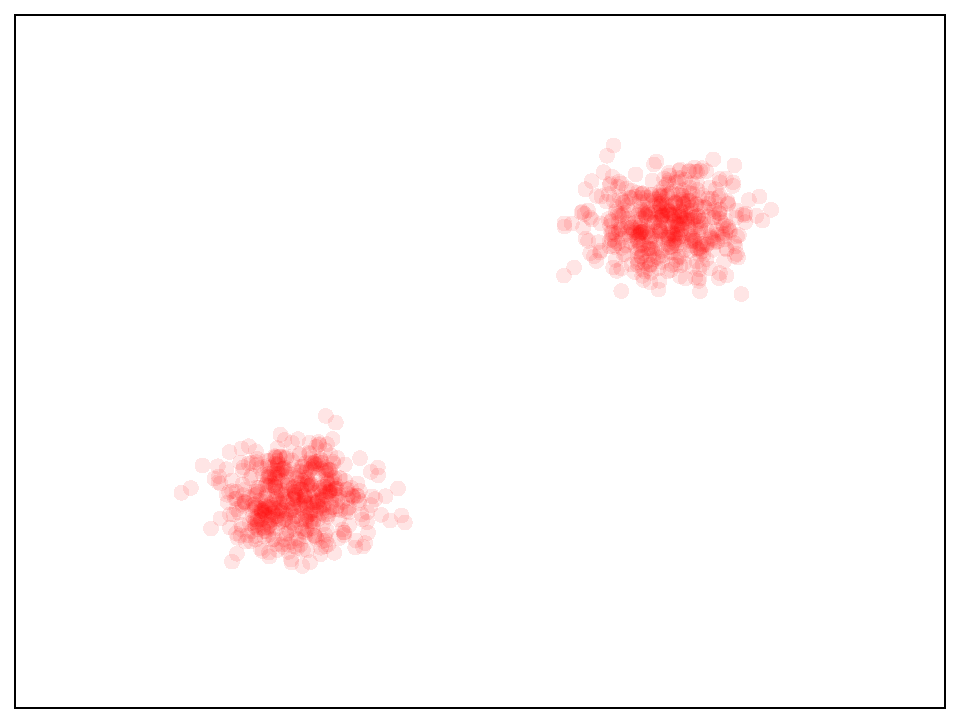
\includegraphics[width=.12\textwidth]{figures/concept_figure/distractors/gt} &
    
\includegraphics[width=.12\textwidth]{figures/concept_figure/distractors/r2omc} &
    
\includegraphics[width=.12\textwidth]{figures/concept_figure/distractors/npec_low} &
    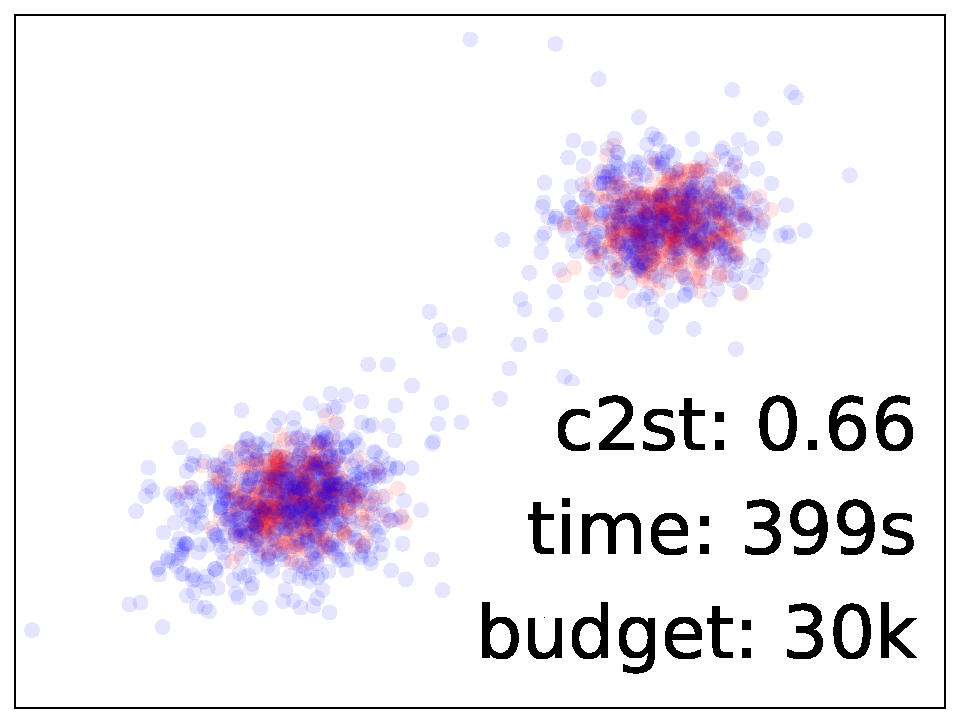
\includegraphics[width=.12\textwidth]{figures/concept_figure/distractors/npec_high} &
    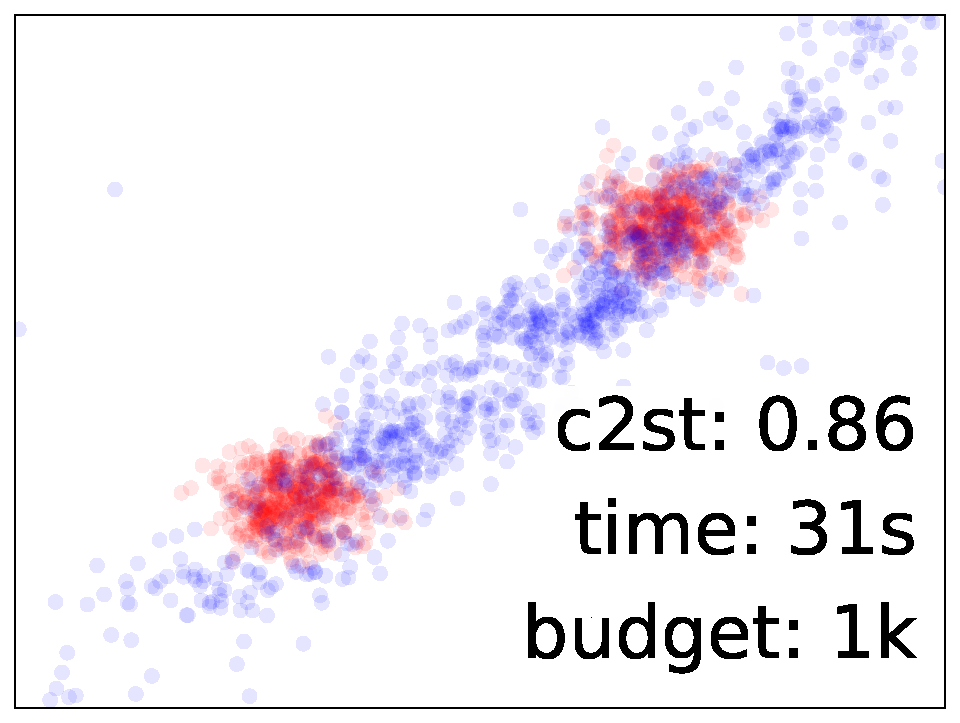
\includegraphics[width=.12\textwidth]{figures/concept_figure/distractors/bayes_flow_low} &
    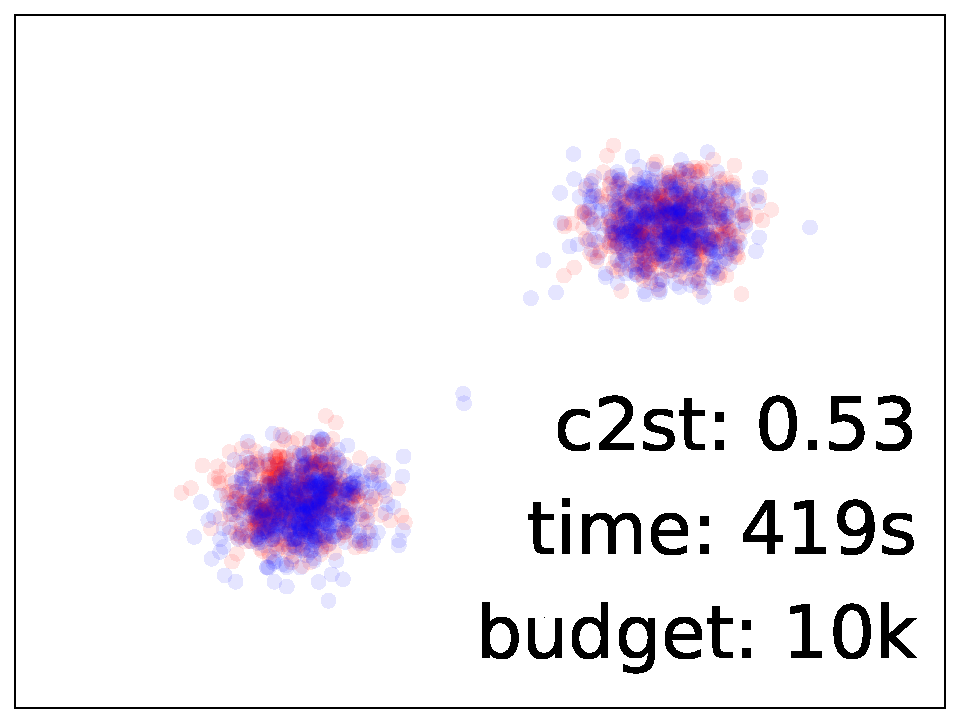
\includegraphics[width=.12\textwidth]{figures/concept_figure/distractors/bayes_flow_high} &
    
\includegraphics[width=.12\textwidth]{figures/concept_figure/distractors/flow_matching_low} &
    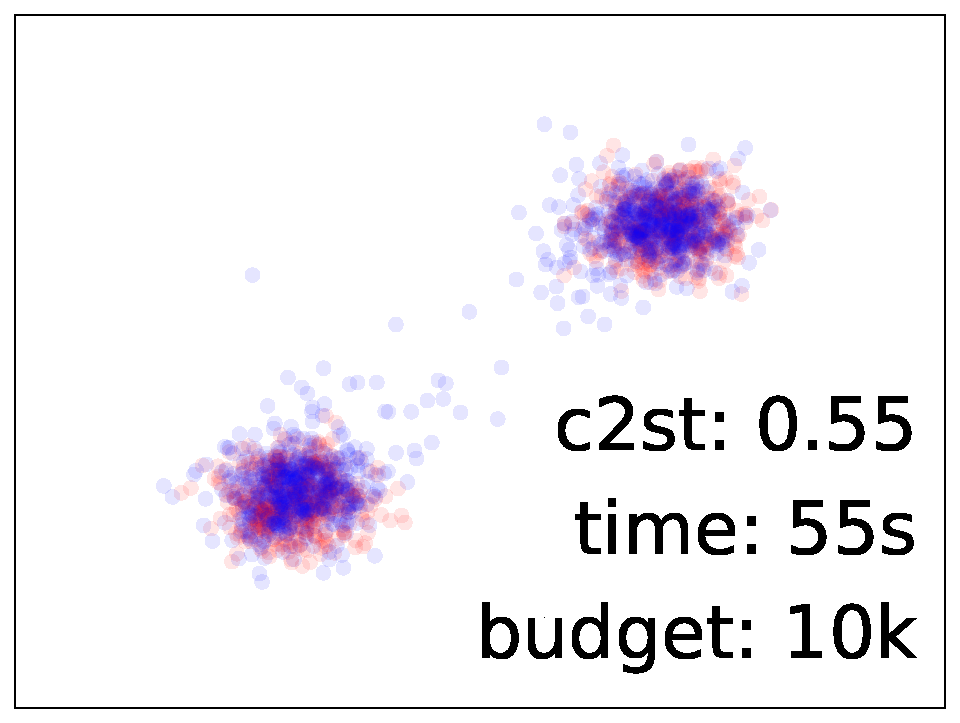
\includegraphics[width=.12\textwidth]{figures/concept_figure/distractors/flow_matching_high} \\
    % Second row example
    \rotatebox{90}{\scriptsize{\; High-dim}} &
    
\includegraphics[width=.12\textwidth]{figures/concept_figure/high_dim/gt} &
    
\includegraphics[width=.12\textwidth]{figures/concept_figure/high_dim/r2omc} &
    
\includegraphics[width=.12\textwidth]{figures/concept_figure/high_dim/npec_low} &
    
\includegraphics[width=.12\textwidth]{figures/concept_figure/high_dim/npec_high} &
    
\includegraphics[width=.12\textwidth]{figures/concept_figure/high_dim/bayes_flow_low} &
    
\includegraphics[width=.12\textwidth]{figures/concept_figure/high_dim/bayes_flow_high} &
    
\includegraphics[width=.12\textwidth]{figures/concept_figure/high_dim/flow_matching_low} &
    
\includegraphics[width=.12\textwidth]{figures/concept_figure/high_dim/flow_matching_high} \\
  \end{tabular}
  \caption{Top to bottom: Simple, high-dimensional, distractors, multiple observations, combined. Left to right: ground truth, NPE, NLE, Naive-ROMC, R2OMC (proposed). Details in Section~\ref{app-sec:intro-example} of the Appendix.}
%   \caption{The simple setup (1) shows two-dimensional marginals for a five-dimensional inference problem, the high-dimensional setup (2) the same for a 20-dimensional problem. Distractors (3) add 10 uninformative dimensions to (1). (4) extends (1) to four iid observations. (5) combines (2-4). Details in Appendices \ref{app-sec:methods} and \ref{app-sec:intro-example}.}
  \label{fig:concept_example}
\end{figure*}

% Key idea of our method: optimization + gradients
We propose a new LFI method that uses gradient information to overcome these challenges.
Building on the Robust Optimization Monte Carlo framework \citep[ROMC,][]{ikonomov2020robust},
we reformulate the stochastic simulation as a set of deterministic optimization problems and use gradient descent to obtain posterior samples.
Gradients, as in standard optimization, provide efficient navigation in high-dimensional parameter spaces, so they rapidly guide us toward high-density posterior regions.
Moreover, they enable sensitivity analyses which allows us to identify and filter out distractor dimensions, thereby improving inference quality.

% Our contributions
The ROMC framework provides the theory for casting inference as deterministic optimization, but, it has two key limitations;
it lacks a strategy for defining an appropriate distance function in problems with distractors or multiple iid observations,
and
its latest implementation~\citep{gkolemis2023extendable} does not exploit gradients or other computational accelerations, which limits its applicability to low-dimensional problems.
We address these challenges with \rromc, an SBI method that when the simulator is differentiable,

\begin{itemize}
 \item enables posterior sampling in high-dimensional parameter spaces under a limited simulation budget,
 \item automatically identifies and filters out uninformative dimensions (distractors),
 \item handles-well multiple iid observations,
 \item runs efficiently through a \texttt{JAX} implementation that uses automatic differentiation, vectorization, and just-in-time compilation.
 \end{itemize}

 \rromc~is systematically compared to state-of-the-art SBI methods, demonstrating accurate posterior inference at a fraction of the computational cost in challenging scenarios.

 \section{Background and Motivation}
 
 Neural–based SBI have demonstrated strong performance on complex simulators, but at the same time they are data-intensive.
 However, their effectiveness typically depends on access to extensive simulated datasets (see Appendix~\ref{app-sec:compute-budget} for details on computational budgets), which makes them slow for two reasons:
 First, generating data from complex simulators is often costly.
 Second, training deep neural networks on high-volume datasets is itself time-consuming.
 % Frequently, it is the latter that constitutes the primary runtime bottleneck \citep{lueckmann2021benchmarking}.
 These long runtimes are a critical limitation, as neural-based methods often require extensive hyperparameter tuning and slow runtimes limit experimental flexibility and practical deployment.

\subsection{ROMC framework}
\label{subsec:ROMC}
ROMC has been introduced by \citet{ikonomov2020robust}, extending and addressing robustness issues of the Optimization Monte Carlo method by \citet{meeds2015optimization}. It belongs to the larger family of ABC methods that approximate the likelihood function as the probability of simulating an output $\epsilon$-close to the observation,
\begin{equation}
L_\epsilon(\thb) = \Pr(d(\yb, \data) \leq \epsilon \mid \thb).
\label{eq:abc_likelihood}
\end{equation}
Here, $d(\cdot, \cdot)$ is a distance, $\yb$ the simulator output, and $\data$ the observed data. In the following, we denote by $g(\thb, \ub)$ the simulator that maps noise (nuisance) variables $\ub \sim p(\ub)$\footnote{In a computer program, sampling $\ub$ corresponds to sampling a random seed.} and parameters $\thb$ to multivariate data $\yb = g(\thb, \ub)$. Introducing the acceptance region $C_\epsilon = \{(\thb, \ub): d(g(\thb, \ub), \data)\le \epsilon\}$ and using the law of the unconscious statistician, (\ref{eq:abc_likelihood}) can be written as
\begin{equation}
    L_\epsilon(\thb) = \E_{p(\ub)}\left[\mathbb{1}_{C_\epsilon}(\thb, \ub) \right],
\end{equation}
where $\mathbb{1}_{C_\epsilon}$ denotes the indicator function that is one if $(\thb, \ub)\in C_\epsilon$ and zero otherwise. When approximating the expectation as a sample average, we obtain
\begin{equation}
    L_\epsilon(\thb) \approx \frac{1}{S} \sum_{i=1}^S \mathbb{1}_{\accregioni}(\thb),
    \label{eq:omc_likelihood}
\end{equation}
which is the proportion of acceptance regions $\accregioni = \{\thb : d(g(\thb, \ub_i), \data) \leq \epsilon \}$ that contain $\thb$.

ROMC takes (\ref{eq:omc_likelihood}) as starting point and focuses on characterizing the acceptance regions $\accregioni$, because once the $\accregioni$ are known, we can not only evaluate the approximate likelihood function, but also obtain posterior samples efficiently. ROMC introduces uniform proposal distributions $q_i$ with support on $\accregioni$ only. Samples from $\thb_{ij} \sim q_i$ for $j \in 1,\ldots, M$, are then equal to posterior samples if weighted with the (unnormalized) weights $w_{ij}$, $i=1, \ldots, S, j=1, \ldots, M$,
\begin{equation}
w_{ij} = \frac{p(\thb_{ij})}{q_i(\thb_{ij})} \mathbb{1}_{C^i_{\epsilon}}(\thb_{ij}) \label{eq:romc_weight}.
\end{equation}

For the characterization of the acceptance regions $\accregioni$, ROMC first determines the minimizers $\thb_i^*$,
\begin{equation}
 \thb_i^* = \text{argmin}_{\thb} d_i(\thb),\quad d_i(\thb) = d(g(\thb, \ub_i), \data),       
 \label{eq:optim_end_points}
\end{equation}

where $d_i(\thb)$ are deterministic distance functions because the sources of randomness (seed) are set to $\ub_i$ and kept fixed.
Next, it starts from the optimization end points $\thb_i^*$ to map out $\accregioni$ using for $\epsilon$ a value derived from the quantiles of the minimial distance functions, $d_i^*=d_i(\thb_i^*), i=1, \ldots, S$ \citep[see][for details]{ikonomov2020robust}. While several options are possible \citep{ikonomov2020robust}, we here use hyperboxes centered at $\thb_i^*$, which can be constructed with a line search algorithm for each parameter dimension. For details, please see Appendix \ref{app-sec:methods}.

The power of the ROMC framework stems from the possibility to use optimization, in particular gradient-based methods, to determine the optimization end points $\thb_i^*$, and hence the acceptance regions $\accregioni$ and the proposal distributions $q_i$. We will exploit this in our method to scale SBI to higher parameter dimensions. Before we can tap into the ROMC framework, however, we will need to overcome challenges related to the definition of the distance function $d$ in case of multiple iid observations and the presence of distractors.

\subsection{ROMC challenges and limitations}
\label{sec:romc-limitations}

ROMC suffers from three main limitations;
(a) it fails in the presence of distractors,
(b) it does not provide a strategy for handling multiple iid observations, and
(c) its existing implementation does not use gradients and other computational accelerations, so it can only be applied to low-dimensional problems.

\paragraph{Uninformative dimensions (distractors).}
\label{sec:romc-limitation-1}

% What are distractors and why we care
Distractors are output dimensions that are unrelated to the parameters of interest.
For example, consider a graphics renderer where the parameter of interest controls a scene element, e.g.\ the appearance of vase, so that most pixel values (output dimensions) are unrelated to the parameter and thus serve as distractors.
% Distractors with a simple example
To emulate distractors consider the simulator of Figure~\ref{fig:concept_example} (second row, more details in Appendix \ref{app-sec:intro-example}).
There, the simulator can be written as $\yb = (\yb^{(1)}, \yb^{(2)})$,
where the first set of dimensions is $ \yb^{(1)} \sim 0.5 \left ( \mathcal{N}(\thb, \mathbf{I}) + \mathcal{N}(-\thb, \mathbf{I}) \right )$,
and the second $\yb^{(2)} \sim \mathcal{N}(\boldsymbol{\mu}, 100\mathbf{I})$, where $\boldsymbol{\mu} \sim \mathcal{U}(-\mathbf{10}, \mathbf{10})$.
In this setup, only $\yb^{(1)}$ depends on $\thb$, while $\yb^{(2)}$ emulates distractors, so, when we observe $\data = (\yb^{o, (1)}, \yb^{o, (2)})$, the true posterior depends solely on $\yb^{o, (1)}$.
% Why ROMC fails with distractors
ROMC is vulnerable to failure in this setting because typical distance functions $d$ consider all output dimensions equally.
Therefore, the minimal distances $d_i^*$ will generally be large for seeds that generate $\yb^{(2)}$ significantly different from $\yb^{o, (2)}$.
This results in an inflated $\epsilon$, and in turn to a much broader posterior than the ground truth.

\begin{figure*}
  \centering
  
\includegraphics[height=.35\linewidth, width=.95\linewidth]{figures/old/concept_image}
  \caption{
    Overview \rromc: Distractors are automatically filtered out and proposal distributions $q_i^n$ are created for each observation (here two): the blue-dotted region indicates where the proposal distributions for the first observation are nonzero, and the green-dotted region indicates the same for the second observation. Only samples that fall within the intersection of both regions are given a positive weight and become posterior samples.}
  \label{fig:concept_image}
\end{figure*}

\paragraph{Multiple iid observations.}

In many applications, we have access to multiple iid observations $\{\data_n\}_{n=1}^N$.
For instance, in neuroscience, researchers often collect multiple recordings of the same neural response to a stimulus.
ROMC does not prescribe a clear strategy for dealing with such cases.
A straightforward approach would be to run the simulator with a different seed $\ub_{i,n}$ for each observation $n$ and then average the distances: $d_i(\thb) = 1/N \sum_n \tilde{d}(g(\thb, \ub_{i,n}), \data_n)$, where $\tilde{d}$ is the distance for a single data point.
However, this approach is sensitive to the ordering of the observations;
the distance increases or decreases artificially if the observations are permuted.
As before, this will generally result in artificially large minimal distances $d_i^*$,
in an excessively large $\epsilon$ and to a much broader posterior than the ground truth.
Other approaches, such as concatenating all observations into a single vector, encounter similar issues.
Note that for squared Euclidean distances, the averaging and concatenation approaches are mathematically equivalent.

\paragraph{Computational efficiency.}

Current ROMC implementations \citep{gkolemis2023extendable} suffer from significant computational bottlenecks that restrict their applicability to low-dimensional problems.
First, optimization relies on gradient-free methods, e.g., Bayesian optimization \citep{snoek2012practical}, which scale poorly with the number of parameters and require many simulator evaluations.
Second, the construction of the acceptance regions $\accregioni$ with a line-search algorithm (see Appendix \ref{app-sec:methods}), require repeated simulator evaluations per seed and per dimension, which also scales poorly with the parameter dimension.

\section{Proposed method: \rromc}
\label{sec:rromc}



We here present our new method for Bayesian parameter inference in simulator models. The method uses gradients to obtain posterior samples even in high-dimensional parameter spaces. The method belongs to the ROMC framework so that we start with discussing how we deal with iid observations and distractors before discussing its implementation.

\subsection{Uninformative dimensions (distractors)}
\label{subsec:distractors}
Distractors can negatively affect the quality of the posterior approximation. To counteract their influence, we measure the sensitivity of the output dimensions with respect to the parameters $\thb$ by computing the average norm of their derivative with respect to $\thb$, and checking that the value is above a minimal value (threshold) $\tau$, 
\begin{equation}
  \label{eq:informative_dimensions}
  I_i = \E_{p(\thb)p(\ub)}\left[ || \nabla_{\thb} g_i(\thb, \ub) || \right] > \tau.
\end{equation}
The expectation equals the expectation with respect to the joint distribution of the prior and the $i$-th dimension of the simulator output, $g_i(\thb, \ub)$. In our experiments, we approximate the expectation using $50$ samples from $p(\thb)$ and $p(\ub)$ each. Collecting all binary indicator variables $I_i$ into the vector $\mask$, we can filter out uniformative dimensions by computing the distance between observed and simulated data for informative dimensions only. To compute $\thb_{i,n}^*$ in (\ref{eq:rromc_optim_end_points}), we minimize
\begin{equation}
d_i^n(\thb) = d(g(\thb, \ub_{i,n})\odot \mask, \data_n \odot \mask).
\label{eq:rromc-masked-distance}
\end{equation}
The procedure is illustrated in Figure~\ref{fig:concept_image}, step (i). 

The threshold $\tau$ controls the sensitivity of the test. In our experiments, we set $\tau$ to machine precision; more sophisticated approaches consist in monitoring the distribution of the expected norm of the gradient, or by assessing false vs true positives under control conditions. This is possible since the mask $\mask$ can be computed prior to receiving observed data.

\subsection{Multiple iid observations}
\label{subsec:multiple-observations}

The likelihood for multiple iid observations $\{\data_n\}_{n=1}^N$ is the product of the likelihoods for each data point. Approximating the likelihood for each data point as in (\ref{eq:omc_likelihood}) and multiplying-in the prior $p(\thb)$, we can obtain a formal expression for the approximate posterior
\begin{equation}
  \label{eq:rromc_posterior}
  p_{\epsilon}(\thb | \{\data_n\}) \propto p(\thb) \prod_{n}^{N} \sum_{i}^S \mathbb{1}_{C_{\epsilon}^{i,n}}(\thb),
\end{equation}
where $C_{\epsilon}^{i,n}$ is the acceptance region for data point $n$ and source of randomness (seed) $\ub_{i,n}$,
\begin{equation}
C_{\epsilon}^{i,n} = \{\thb : d(g(\thb, \ub_{i,n}), \data_n) \leq \epsilon \}.
\end{equation}
We have $S$ sources of randomness for each data point $\data_n$, and so in total $S*N$ acceptance regions $C_{\epsilon}^{i,n}$.

We now address the question how to efficiently sample from $p_{\epsilon}(\thb | \{\data_n\})$. To achieve this, we consider the task of computing the posterior expectation $\bar{h} = \E_{p_{\epsilon}}[h(\thb)]$ under $p_{\epsilon}(\thb | \{\data_n\})$. Plugging in the expression in (\ref{eq:rromc_posterior}) gives, after normalization,
\begin{equation}
  \label{eq:rromc_expectation}
  \bar{h} = \frac{ \int h(\thb) p(\thb) \prod_n^N \sum_i^S \mathbb{1}_{C_{\epsilon}^{i,n}}(\thb) d\thb}{\int p(\thb) \prod_n^N \sum_i^S \mathbb{1}_{C_{\epsilon}^{i,n}}(\thb) d\thb}.
\end{equation}

The integrals in the equation are typically intractable. But they correspond to expectations with respect to the prior $p(\thb)$ and hence could be approximated with a sample average. However, this is very inefficient. Few (or no) prior samples will generate outputs $\epsilon$-close to all observations, so most (or all) will get zero weight, leading to a very low effective sample size. Following the general ROMC framework by \citet{ikonomov2020robust}, we thus employ importance sampling with an adaptive proposal distribution obtained via optimization. 

We first treat each data point $\data_n$ separately and construct proposal distributions $q_i^n(\thb)$, $i=1, \ldots, S$, as in Section \ref{subsec:ROMC}: We use optimization to find the minimizers $\thb_{i,n}^*$ of the deterministic functions $d_i^n(\thb) = d(g(\thb, \ub_{i,n}), \data_n)$,       
\begin{equation}
 \thb_{i,n}^* = \text{argmin}_{\thb} d_i^n(\thb),
 \label{eq:rromc_optim_end_points}
\end{equation}
and then build a hyperbox around each acceptance region $C_{\epsilon}^{i,n}$ and define $q_i^n(\thb)$ to be the uniform distribution over it. The optimization problem in (\ref{eq:rromc_optim_end_points}) is deterministic and we solve it with gradient-based methods to enable scalability to large parameter spaces. Note that treating each data point $\data_n$ separately allows us to avoid the issues explained in Section \ref{sec:romc-limitations}.

We propose to combine the per-data point proposal distributions $q_i^n(\thb)$ in form of a mixture distribution,
\begin{equation}
    q(\thb) = \frac{1}{N} \frac{1}{S} \sum_{n=1}^N \sum_{i=1}^S q_i^n (\thb).
    \label{eq:R2OMC-proposal}
\end{equation}
The posterior expectation in (\ref{eq:rromc_expectation}) can then be approximated in form of a weighted average 
\begin{equation}
  \label{eq:rromc_sample_expectation}
  \bar{h} = \frac{\sum_p w_p h(\thb_p)}{\sum_p w_p}, \quad \thb_p \sim q(\thb)
\end{equation}
where the weights $w_p$, $p=1, \ldots, P$, are given by
\begin{equation}
  \label{eq:rromc_weight}
w_p= \frac{p(\thb_p)}{q(\thb_p)} \prod_{n=1}^N \sum_{i=1}^S \mathbb{1}_{C_{\epsilon}^{i,n}}(\thb_p). 
\end{equation}
This means that the $\thb_p \sim q(\thb)$, weighted by $w_p$, represent samples from the posterior $p_{\epsilon}(\thb | \{\data_n\})$ in (\ref{eq:rromc_posterior}).

The rationale for choosing $q(\thb)$ in (\ref{eq:R2OMC-proposal}) as proposal distribution is as follows: it is a mixture of uniform distributions, so sampling and evaluating is easy. It seamlessly combines the contribution from multiple data points, allowing future data points to be included without re-computation. If each $q_i^n$ encloses the corresponding acceptance region $C_{\epsilon}^{i,n}$, then $q(\thb) > 0$ in areas of the parameter space where $\prod_n^N \sum_i^S \mathbb{1}_{C_{\epsilon}^{i,n}}(\thb) > 0$ and no posterior mass is discarded in the weighting in (\ref{eq:rromc_weight}). Finally, regions of high likelihood are characterized by regions where multiple $C_{\epsilon}^{i,n}$ overlap. As the proposal distribution $q(\thb)$ consists of a mixture of the $q_i^n(\thb)$ with equal weights, areas where multiple $C_{\epsilon}^{i,n}$ overlap will be sampled more often, so that areas of high likelihood will be represented with more samples.

Figure~\ref{fig:concept_image}, steps (ii-iii), illustrates the proposed procedure to obtain posterior samples. We have two observed data points and the $\thb_p$ come from regions that match at least one observation; the blue-dotted area for $\data_1$ and the green-dotted region for $\data_2$. However, only the ones that match both will get a positive weight (red dots) and become posterior samples.

\begin{figure*}[!t]
  \centering
  \begin{subfigure}[b]{0.245\textwidth}
    
\includegraphics[width=\linewidth]{./figures/mog_benchmark/single_mode/c2st_frontier}
    \caption{$S_{\mathtt{base}}$}
  \end{subfigure}
  \begin{subfigure}[b]{0.245\textwidth}
    
\includegraphics[width=\linewidth]{./figures/mog_benchmark/single_mode_distractors/c2st_frontier}
    \caption{$S_{\mathtt{base}}^{\mathtt{dist}}$}
  \end{subfigure}
  \begin{subfigure}[b]{0.245\textwidth}
    
\includegraphics[width=\linewidth]{./figures/mog_benchmark/two_modes/c2st_frontier}
    \caption{$S_{\mathtt{MoG}}$}
  \end{subfigure}
  \begin{subfigure}[b]{0.245\textwidth}
    
\includegraphics[width=\linewidth]{./figures/mog_benchmark/two_modes_distractors/c2st_frontier}
    \caption{$S^{\mathtt{dist}}_{\mathtt{MoG}}$}
  \end{subfigure}
  \caption{MoG benchmark: Success Frontier plots showing the lowest budget required to reach a C2ST score $\leq 0.75$ for varying $D$.}
  \label{fig:high_dim_benchmark}
\end{figure*}



\subsection{\texttt{JAX} implementation}
\label{subsec:implementation}

Algorithms~\ref{alg:r2omc} summarizes the key steps of \rromc. It has three steps: dealing with distractors (line 2); constructing per-data point proposal distributions $\{q_i^n\}_{i=1}^S$ (lines 4-5); combining them to form the overall proposal distribution $q(\thb)$ and generating the weighted samples (lines 7-8).

\begin{algorithm}[!ht]
  \caption{\texttt{R2OMC}. Requires: $p(\thb), g(\thb, \ub), \{\data_n\}_{n=1}^{N}$}
  \label{alg:r2omc}
  \begin{algorithmic}[1]
    \Procedure{\rromc}{$\tau, S, P$}
      \State $\mask = (I_1, \ldots, I_{D_{y}})$ using~(\ref{eq:informative_dimensions}) with $\tau$ 
      \For{\(n \gets 1 \textrm{ to } N\)}
      \State $\thb_{i,n}^* = \text{argmin}_{\thb} d_i^n(\thb)$ using (\ref{eq:rromc-masked-distance}) for all $i$
      \State Compute hyperboxes and $\{q_i^n\}_{i=1}^S$
    \EndFor
    \State $\thb_p \sim q(\thb)$, where $ q(\thb)= \frac{1}{N} \frac{1}{S} \sum_n \sum_i q_i^n (\thb)$
    \State Compute $\{w_p\}_p^P $ using (\ref{eq:rromc_weight})
    \State \Return $\{w_p, \thb_p\}_{p=1}^{P}$ 
    \EndProcedure
  \end{algorithmic}
\end{algorithm}

We offer an efficient \texttt{JAX} implementation, benefiting from automatic differentiation (\texttt{grad}), vectorization (\texttt{vmap}), and just-in-time compilation (\texttt{jit}). 
In many cases, \rromc~executes in seconds where most SBI methods require minutes (see Section~\ref{sec:experiments}). 

\rromc~requires approximately $N * S$ evaluations of the simulator: For the distractors, \texttt{grad} computes $\partial g_i/\partial \theta_j$ for all $i$ and $j$ in one call, and \texttt{vmap} evaluates multiple $\thb$ at once.
Combining them, the cost is $S$. Obtaining the per-data point proposal distributions $\{q_i^n\}_{i=1}^S$ consists of optimization (line 4) and hyperbox building (line 5) for each data point. Each of $S$ optimizations requires $T$ gradient descent steps, where $T$ is a user-defined hyperparameter. \texttt{jit} allows compiling $T_1$ consequtive steps to apply them at the cost of a single execution, so the cost reduces to $S \frac{T}{T_1}$. $\frac{T}{T_1}$ is normally small, and can even reach $1$ if memory allows setting $T_1 = T$. Hyperbox building also requires of the order of $S$ steps when the required line searches are parallelized over each parameter dimensions using \texttt{vmap} (see Appendix \ref{app-sec:methods}). Thus the total cost of this step is of the order of $N*S$. For generating the weighted samples, (\ref{eq:rromc_weight}) is evaluated on $P$ samples (line 8).
The simulator is only used for computing $\prod_n^N \sum_i^S \mathbb{1}_{C_{\epsilon}^{i,n}}(\thb_p)$ which requires evaluating $S * N$ different distance functions on $P$ points each. Using \texttt{vmap} in each distance function, the total cost is $S * N$. Evaluating $q(\cdot)$ and $p(\cdot)$ does not require calling the simulator. Finally, if the simulator is expensive, the $S *N$ cost of checking whether the samples are in the acceptance regions can be avoided by using the hyperbox or another model for the acceptance region, see \citet{ikonomov2020robust}. 

The code is available at \LinkToCode.

\subsection{Discussion - Limitations}

\section{Experiments}
\label{sec:experiments}

To assess \rromc, we conduct experiments on a Mixture of Gaussians benchmark, on the synthetic SBI benchmark and an image-based inference problem, covering scenarios with high-dimesional data, distractors, multiple observations and complex posterior shapes.

\paragraph{Methods.}

In the MoG benchmark, we compare \rromc~against three well-known neural methods: \NPE~\citep{greenberg2019automatic}, BayesFlow~\citep{radev2020bayesflow} and FlowMatching~\citep{wildberger2023flow}.
We use our \texttt{JAX} implementation for \rromc and for the competitors the implementation provided by the \texttt{SBI Pytorch} package.
In the SBI benchmark, we compare \rromc~against all methods reported by \citet{lueckmann2021benchmarking}.
% i.e., Rejection ABC (\REJ), Sequential Monte Carlo ABC (\SMC), Neural Likelihood Estimation (\NLE), Neural Ratio Estimation (\NRE), and their sequential variants.
In the image-based inference problem, we illustrate the applicability of \rromc~to a high-dimensional real-world problem, without comparing it.
All experiments were conducted on a single Dell XPS PC equipped with an Intel® Core™ i7-10750H CPU @ 2.60GHz with 12 cores.
Appendix~\ref{app-sec:experiments} contains further details on the setup and methods.

\paragraph{Metrics.}

All methods are evaluated with the \CtwoST~score~\citep{gutmann2018likelihood, lueckmann2021benchmarking}, which uses classification to measure the similarity between two sets; the first set are the samples from the approximate posterior and the second set from the ground truth. The best score is $0.5$, indicating that the two sets are indistinguishable, while the worst score is $1.0$, indicating perfect separation.
As classifier, we use a fully-connected neural network trained on $1,000$ samples from each set and report the mean \CtwoST~score over $5$ independent runs.

\subsection{MoG benchmark}
\label{subsec:gaussian}

We systematically evaluate SBI methods when the dimensionality of the parameter space $D$ increases.
We use two simulators,
$S_{\mathtt{base}}: \yb \sim \mathcal{N}(\thb, \sigma^2 \mathbf{I})$ and
$S_{\mathtt{MoG}}: \yb \sim \frac{1}{2}\left ( \mathcal{N}(\thb, \sigma_1^2 \mathbf{I}) + \mathcal{N}(-\thb, \sigma_2^2\mathbf{I})\right)$, that lead to uni-modal and bi-modal posteriors respectively.
For each simulator, we consider a simple version, where the output has the same dimensionality as the parameter vector ($D_y = D$), and a distractor version, where where we append $100$ uninformative dimensions to the output ($D_y = D + 100$).
The distractor dimensions are sampled from $\mathcal{N}(\boldsymbol{\mu}, 100 \mathbf{I})$, with $\boldsymbol{\mu} \sim \mathcal{U}(-10, 10)$.
That is, we consider four simulators in total.

As observed data, we use $\data_n \approx (5, \ldots, 5)$, that is a vector of 5's with some small noise around it.
In case of distractors, we append $100$ zeros to it. 
The posterior for $S_{\mathtt{base}}$ is then approximated by a truncated Gaussian, while the posterior for $S_{\mathtt{MoG}}$ is well approximated by a truncated bi-modal Gaussian.

For each simulator, we evaluate \rromc~against the three neural methods mentioned above, varying $D$ from $2$ to $20$ and the simulation budget from $1\_000$ to $100\_000$.
For all simulators, we use $\mathcal{U}(\mathbf{-3}, \mathbf{3})$ as prior.
For more details on the setup, see Appendix \ref{app-sec:experiments}.

Figure~\ref{fig:high_dim_benchmark} summarizes the results in form of Success Frontier plots, showing the lowest budget required for a successful inference, defined as reaching a \CtwoST~score $\leq 0.75$, for varying $D$.
All neural-based methods follow the same trend; as $D$ increases, so does the requird budget, and soon they ask for more than $100\_000$ simulations to succeed, which incurs very high runtimes (see Appendix \ref{app-sec:experiments}).
They struggle more with $S_{\mathtt{MoG}}$ than with $S_{\mathtt{base}}$, as the posterior is more complex and more on the distractor versions than on the simple ones.
In contrast, \rromc~succeeds with a budget of up to $1\_000$ simulations and a runtime of a few seconds for all $D$ and all simulators.

\subsection{SBI benchmark}
\label{subsec:sbi-benchmark}

The SBI~\citep{lueckmann2021benchmarking} is a widely used benchmark for SBI methods.
We select two characteristic experiments from the benchmark that cover different challenges.

\subsubsection{SLCP (T.3) and plus distractors (T.4)}

\begin{figure}
    \centering
    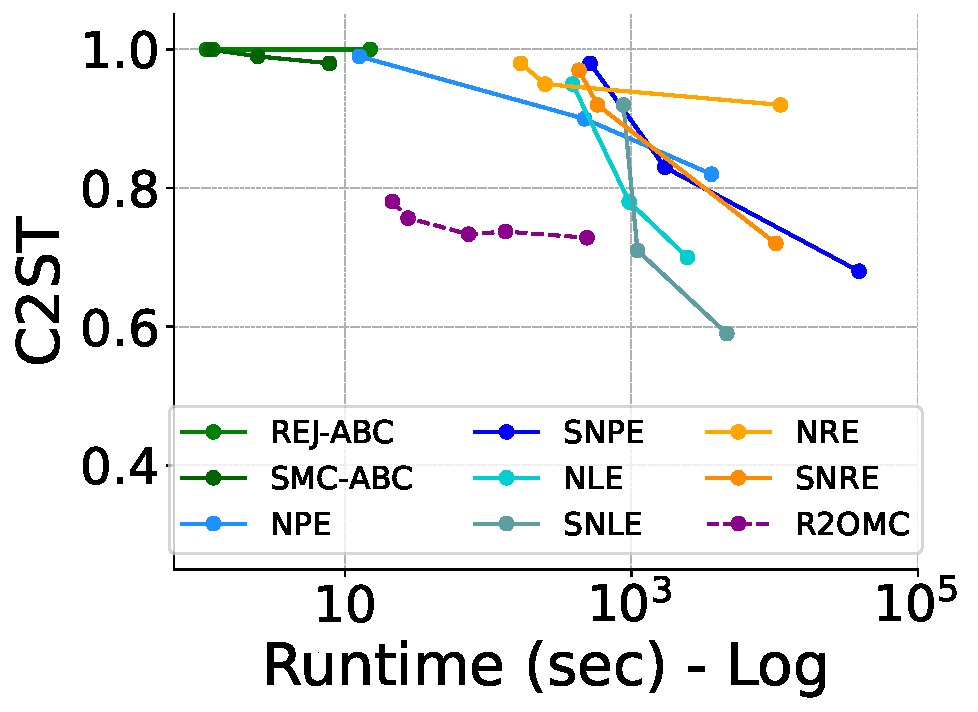
\includegraphics[width=.49\linewidth]{./figures/sbibm/slcp/c2st_vs_runtime}
    
\includegraphics[width=.49\linewidth]{./figures/sbibm/slcp_distractors/c2st_vs_runtime}
    \caption{SLCP (left) and SLCP with distractors (right): C2ST score vs. runtime.}
    \label{fig:slcp_c2st_runtime}
\end{figure}

\begin{figure}
    \centering
    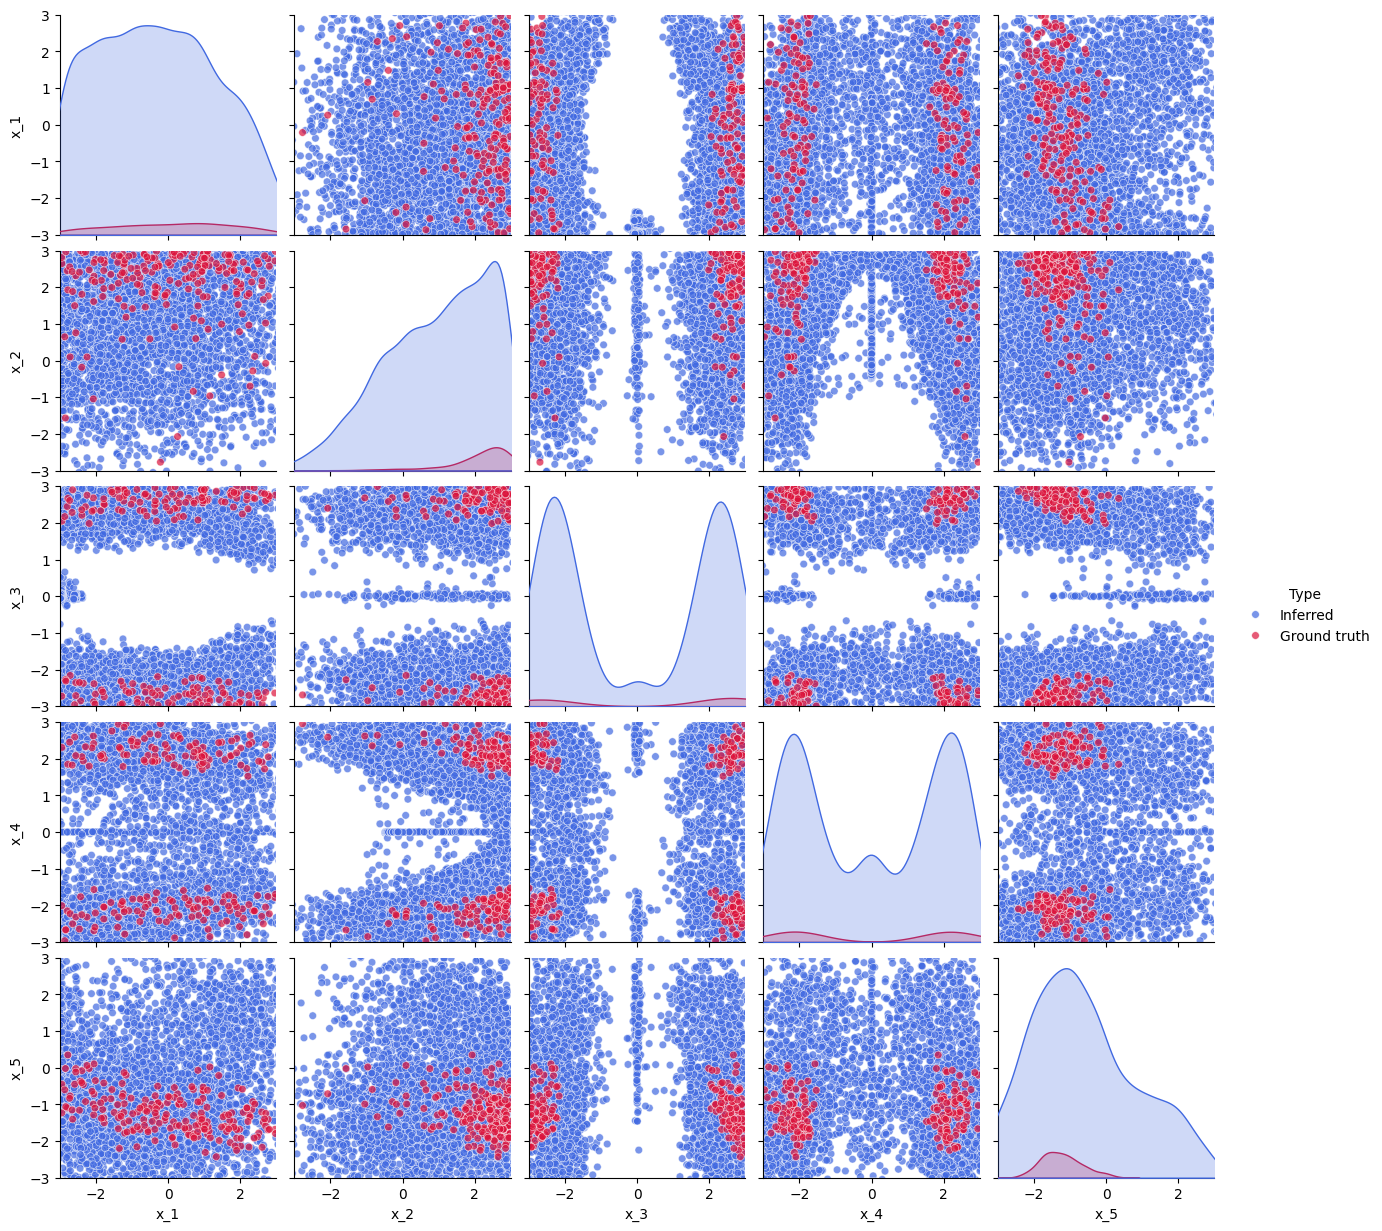
\includegraphics[width=.49\linewidth]{figures/sbibm/slcp/pairwise_posterior_total}
    
\includegraphics[width=.49\linewidth]{figures/sbibm/slcp/pairwise_posterior_selected}
    \caption{SLCP pairwise posteriors: using all proposal samples (left) and only the selected ones (right).}
    \label{fig:slcp_posterior}
\end{figure}

The SLCP (Simple Likelihood, Complex Posterior) task has a uniform prior over five parameters $\thb \in \mathcal{U}(-\mathbf{3}, \mathbf{3})^5$ and
four two-dimensional observations drawn from a Gaussian distribution whose mean and variance are nonlinear functions of~$\theta$.
This creates a posterior with four symmetric modes and sharp vertical cut-offs.
SLCP with distractors augments the original SLCP task, adding 92 non-informative dimensions for a total of a $100$D output.

Figure~\ref{fig:slcp_c2st_runtime} shows \CtwoST score versus runtime for \rromc and methods from \citet{lueckmann2021benchmarking} on both SLCP variants.
\rromc~achieves accurate posterior approximation (\CtwoST~score $0.7$--$0.8$) in seconds using a budget of $10^3$ samples.
Other methods require significantly longer runtimes (up to hours) and budgets of at least $10^4$ (often $10^5$) samples for similar performance.
Results are more pronounced with distractors, where most methods fail to reach \CtwoST~scores below $0.8$ regardless of budget.

Figure~\ref{fig:slcp_posterior} illustrates \rromc ability to handle multiple observations by using the weighting scheme in \rromc (Eq.\ref{eq:rromc_weight}).
The left panel shows pairwise posteriors using all proposal samples, i.e., the ones that are in $\epsilon$-distance per observation, and represent a much broader distribution.
Out of them, only the ones that are in $\epsilon$-distance to all observations are given a positive weight and become posterior samples, as shown in the right panel.

\subsubsection{Two-moons (T.8)}

\begin{figure}
    \centering
    
\includegraphics[width=.49\linewidth]{figures/sbibm/two_moons/c2st_vs_runtime}
    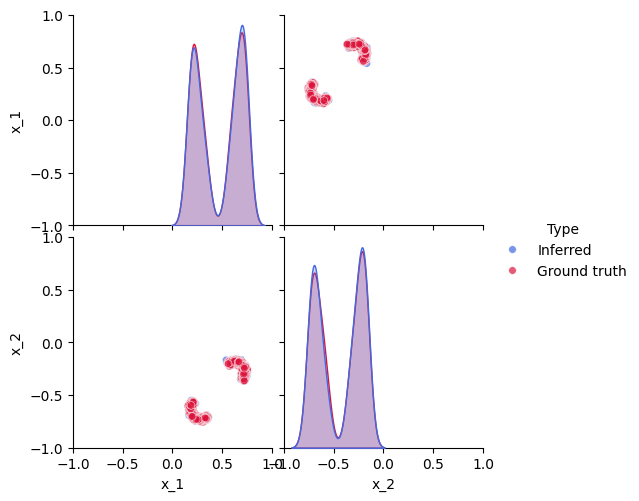
\includegraphics[width=.49\linewidth]{figures/sbibm/two_moons/pairwise_posterior}
    \caption{
      Two-moons results: C2ST score vs. runtime (Left) and pairwise posterior (Right).
    }
    \label{fig:sbi_two_moons}
\end{figure}

\begin{figure}
  \centering
  \resizebox{\linewidth}{!}{%
      \setlength{\tabcolsep}{1pt}
      \renewcommand{\arraystretch}{2}
      \begin{tabular}{*{10}{c} >{\centering\arraybackslash}m{0.1\textwidth}}
          \imagerow{images/image_pixelwise}{image_clean}{Clean: $\thb^*$}
          \hline
          \imagerow{images/image_pixelwise}{image_observation}{Observed: $\data$}
          \imagerow{images/image_pixelwise}{posterior_mean}{Posterior mean}
          \imagerow{images/image_pixelwise}{posterior_std}{Posterior std}
          \hline
          \imagerow{images/image_checkerboard}{image_observation}{Observed: $\data$}
          \imagerow{images/image_checkerboard}{posterior_mean}{Posterior mean}
          \imagerow{images/image_checkerboard}{posterior_std}{Posterior std}
      \end{tabular}
    }
  \caption{
    Image-based inference results.
    Top row shows the clean ground truth image $\thb^*$. 
    Rows 2--4 display the distorted observation, posterior mean, and posterior standard deviation 
    obtained by~\rromc for pixel-wise distortion.
    Rows 5--7 show the same results for the edge-detection filter distortion.
  }
  \label{fig:pixelwise}
\end{figure}

The 2-moons task tests whether the methods can estimate posteriors with bimodal and crescent shape structure.
The simulator is $\yb|\thb \sim  (r\cos(\alpha) + 0.25, r \sin(\alpha)) + (-|\theta_1 + \theta_2| / \sqrt{2}, (-\theta_1 + \theta_2) / \sqrt{2})$ with $\alpha \sim \mathcal{U}(-\pi/2, \pi/2)$ and $r \sim \mathcal{N}(0.1, 0.01^2)$.
The dimensionality is $D=2$ and the prior is $\thb \sim \mathcal{U}(\mathbf{-1}, \mathbf{1})$,
creating a posterior with two half-moon shape modes.

Figure~\ref{fig:sbi_two_moons} shows the \CtwoST~score and the pairwise posterior of \rromc~and all methods from \citet{lueckmann2021benchmarking}.
\rromc~achieves a \CtwoST close to $0.5$ with a runtime of a few seconds (budget of $10^3$ samples),
whereas other methods require much longer runtimes (minutes to hours) to reach a similar score (budget of $10^5$ samples).
Additional results showing the scores vs. budget are in Appendix~\ref{app-sec:experiments}.
The pairwise posterior shows that \rromc~accurately captures the two crescent-shaped modes of the posterior.

\subsection{Image-based inference}
\label{subsec:image-based}

We evaluate \rromc~on (very) high-dimensional parameter spaces through image inference in noisy camera models.
Two simulators are tested on MNIST dataset observations~\citep{lecun1998gradient}.
The first applies pixel-wise intensity changes, $y_{ij} = a\theta_{ij} + b + \boldsymbol{\epsilon}$,
where $\theta_{ij}$ is pixel intensity and $a$ and $b$ control contrast and brightness.
The second applies edge-detection filtering, $\yb = \text{filter}(\thb) + \boldsymbol{\epsilon}$,
using convolution with $\text{filter}(\cdot)$.
Both use Gaussian noise $\boldsymbol{\epsilon} \sim \mathcal{N}(\mathbf{0}, 0.1^2 \mathbf{I})$ and
uninformative prior $\thb \sim \mathcal{U}(0,1)^{28 \times 28}$.

Figure~\ref{fig:pixelwise} shows that for both simulators,
the posterior mean obtained by~\rromc visually resembles to the original clean image,
indicating that the posterior mode is close to the true generating parameter $\thb^*$.
SBI inference on images is highly difficult due to the curse of dimensionality.
Few methods like GATSBI~\citep{ramesh2022gatsbi} succeed but require complex generative models with long, and often unstable, training.
In contrast, \rromc~achieves accurate inference with only $100$ simulations and a runtime of a few seconds.


\section{Conclusion}
\label{sec:conclusion}

We have presented \rromc, a new Bayesian inference method for simulator models that addresses three key scalability challenges in simulation-based (likelihood-free) inference, namely high-dimensional parameter spaces, multiple observations, and the possible presence of uninformative dimensions (i.e., distractors). R2OMC builds on the ROMC framework and formulates the inference problem in terms of a set of deterministic optimization problems that can be solved with gradient-descent, enabling inference in high-dimensional parameter spaces. It further introduces a gradient-based filtering step to mask distractors during inference. It uses a novel adaptive importance sampling approach that efficiently identifies posterior samples that explain \emph{all} available iid observations. We offer an efficient \texttt{JAX}-based implementation that leverages key auto-differentiation and vectorization features to accelerate the inference. Simulations performed with novel experimental settings as well as the comprehensive SBI benchmark show that R2OMC achieves improved accuracy (close to the optimal $0.5$ \texttt{C2ST}) compared to existing methods, while using a smaller number of simulator calls and a fraction of the computational time. 


% The results are very promising; even without any methodological improvements, ROMC seems to perform much beyond the state-of-the-art most problems. I discuss below the limitations we can focus on.

% \subsection{Multiple Observations}

% When dealing with multiple observations (as in the SLCP problem) $\data = [\data_1, \cdots, \data_N]$, the OMC scheme doesn't perform well. This is because we are not optimizing over unobserved (latent) variables.

% For example, suppose we have a latent variable $k$ drawn from a Bernoulli distribution, $k \sim \mathcal{B}(0.5)$. When $k=0$, the observation is then sampled from $\mathcal{N}(-\thb, \mathbf{I})$, and when $k=1$, it's sampled from $\mathcal{N}(\thb, \mathbf{I})$. Let's say we have two observations $\data_1 = (5.1, 4.9)$ and $\data_2 = (-5, -5.1)$. The ground truth posterior has two gaussian modes with centers around $\pm (5, 5)$.

% However, if we apply OMC as is, meaning optimizing over a flat vector of observations $\data = (5.1, 4.9, -5, -5.1)$, it will give a Gaussian with a center at $(0,0)$ and high covariance.

% \paragraph{Ideas.}

% Optimize independently for each observation, meaning for $\mathtt{seed}[i]$, optimize separately for $\data_1$ and $\data_2$, and accept two bounding boxes, one for each observation.
% Does this approach makes sense? If so, could we show it theoretically as well?

% \subsection{Epsilon thresholds}

% ROMC works with three acceptance thresholds: \(\epsilon_1\) for accepting \(\thb_*\), \(\epsilon_2\) for the proposal area, and \(\epsilon_3\) for accepting samples. Setting these thresholds is not straightforward; in problems with distractors, the distance to the observation is heavily influenced by them. As a result, certain seeds have much smaller distances than others, leading to larger proposal areas and dominating the posterior, regardless of the \(\epsilon_2\) threshold.

% \paragraph{Ideas.}


% \subsection{Hybrid Schema}

% ROMC is only capable of sampling from the posterior distribution. It would be intresting to propose a solution that not only samples from the posterior but also models it, meaning it provides a $\mathtt{.log\_prob()}$ method in addition to $\mathtt{.sample()}$.

% \paragraph{Ideas.}
% The initial idea was to utilize ROMC as the first step in supplying training samples for neural-based SBI methods. This approach would render the hybrid method $\epsilon$-free, addressing some of the discussed issues. The concept relies on the observation that NRE, NPE, and NLE perform significantly better in their sequential versions, where the proposal area is updated sequentially to mimic the posterior distribution. \textbf{However, I encountered difficulties in making this approach effective; I attempted to train NPE using the samples provided by ROMC but didn't observe significant improvement, except in the case of the linear Gaussian example.}

% Interestingly, simply fitting a Mixture of Gaussians (MoG) yielded much better results. However, MoG has the limitation that the user needs to manually determine the number of components, which is challenging without intuition about the posterior's shape. In the current experiments, setting it to 50 seems to work well.

% \subsection{More experiments.}

% I want to test ROMC in more problems.

% \paragraph{Ideas.}

% The SLCP example will demonstrate how the method performs with multiple observations when the posterior is multi-modal and asymmetric.
% A series of problems involving distractors will examine whether the method can identify uninformative dimensions of the observation.
% Regarding real-case problems, the SBI Benchmark includes SIR and Lotka-Volterra, but I'm unsure if the simulator is differentiable in these cases. If not, we need to find additional examples.

\clearpage

\bibliographystyle{unsrtnat}
\bibliography{paper}
% \section{GENERAL FORMATTING INSTRUCTIONS}

% Submissions are limited to \textbf{8 pages} excluding references. 
% There will be an additional page for camera-ready versions of the accepted papers.

% Papers are in 2 columns with the overall line width of 6.75~inches (41~picas).
% Each column is 3.25~inches wide (19.5~picas).  The space
% between the columns is .25~inches wide (1.5~picas).  The left margin is 0.88~inches (5.28~picas).
% Use 10~point type with a vertical spacing of
% 11~points. Please use US Letter size paper instead of A4.

% Paper title is 16~point, caps/lc, bold, centered between 2~horizontal rules.
% Top rule is 4~points thick and bottom rule is 1~point thick.
% Allow 1/4~inch space above and below title to rules.

% Author descriptions are center-justified, initial caps.  The lead
% author is to be listed first (left-most), and the Co-authors are set
% to follow.  If up to three authors, use a single row of author
% descriptions, each one center-justified, and all set side by side;
% with more authors or unusually long names or institutions, use more
% rows.

% Use one-half line space between paragraphs, with no indent.

% \section{FIRST LEVEL HEADINGS}

% First level headings are all caps, flush left, bold, and in point size
% 12. Use one line space before the first level heading and one-half line space
% after the first level heading.

% \subsection{Second Level Heading}

% Second level headings are initial caps, flush left, bold, and in point
% size 10. Use one line space before the second level heading and one-half line
% space after the second level heading.

% \subsubsection{Third Level Heading}

% Third level headings are flush left, initial caps, bold, and in point
% size 10. Use one line space before the third level heading and one-half line
% space after the third level heading.

% \paragraph{Fourth Level Heading}

% Fourth level headings must be flush left, initial caps, bold, and
% Roman type.  Use one line space before the fourth level heading, and
% place the section text immediately after the heading with no line
% break, but an 11 point horizontal space.

% %%%
% \subsection{Citations, Figure, References}


% \subsubsection{Citations in Text}

% Citations within the text should include the author's last name and
% year, e.g., (Cheesman, 1985). 
% %Apart from including the author's last name and year, citations can follow any style, as long as the style is consistent throughout the paper.  
% Be sure that the sentence reads
% correctly if the citation is deleted: e.g., instead of ``As described
% by (Cheesman, 1985), we first frobulate the widgets,'' write ``As
% described by Cheesman (1985), we first frobulate the widgets.''


% The references listed at the end of the paper can follow any style as long as it is used consistently.

% %Be sure to avoid
% %accidentally disclosing author identities through citations.

% \subsubsection{Footnotes}

% Indicate footnotes with a number\footnote{Sample of the first
%   footnote.} in the text. Use 8 point type for footnotes. Place the
% footnotes at the bottom of the column in which their markers appear,
% continuing to the next column if required. Precede the footnote
% section of a column with a 0.5 point horizontal rule 1~inch (6~picas)
% long.\footnote{Sample of the second footnote.}

% \subsubsection{Figures}

% All artwork must be centered, neat, clean, and legible.  All lines
% should be very dark for purposes of reproduction, and art work should
% not be hand-drawn.  Figures may appear at the top of a column, at the
% top of a page spanning multiple columns, inline within a column, or
% with text wrapped around them, but the figure number and caption
% always appear immediately below the figure.  Leave 2 line spaces
% between the figure and the caption. The figure caption is initial caps
% and each figure should be numbered consecutively.

% Make sure that the figure caption does not get separated from the
% figure. Leave extra white space at the bottom of the page rather than
% splitting the figure and figure caption.
% \begin{figure}[h]
% \vspace{.3in}
% \centerline{\fbox{This figure intentionally left non-blank}}
% \vspace{.3in}
% \caption{Sample Figure Caption}
% \end{figure}

% \subsubsection{Tables}

% All tables must be centered, neat, clean, and legible. Do not use hand-drawn tables.
% Table number and title always appear above the table.
% See Table~\ref{sample-table}.

% Use one line space before the table title, one line space after the table title,
% and one line space after the table. The table title must be
% initial caps and each table numbered consecutively.

% \begin{table}[h]
% \caption{Sample Table Title} \label{sample-table}
% \begin{center}
% \begin{tabular}{ll}
% \textbf{PART}  &\textbf{DESCRIPTION} \\
% \hline \\
% Dendrite         &Input terminal \\
% Axon             &Output terminal \\
% Soma             &Cell body (contains cell nucleus) \\
% \end{tabular}
% \end{center}
% \end{table}

% \section{SUPPLEMENTARY MATERIAL}

% If you need to include additional appendices during submission, you can include them in the supplementary material file.
% You can submit a single file of additional supplementary material which may be either a pdf file (such as proof details) or a zip file for other formats/more files (such as code or videos). 
% Note that reviewers are under no obligation to examine your supplementary material. 
% If you have only one supplementary pdf file, please upload it as is; otherwise gather everything to the single zip file.

% You must use \texttt{aistats2025.sty} as a style file for your supplementary pdf file and follow the same formatting instructions as in the main paper. 
% The only difference is that it must be in a \emph{single-column} format.
% You can use \texttt{supplement.tex} in our starter pack as a starting point.
% Alternatively, you may append the supplementary content to the main paper and split the final PDF into two separate files.

% \section{SUBMISSION INSTRUCTIONS}

% To submit your paper to AISTATS 2025, please follow these instructions.

% \begin{enumerate}
%     \item Download \texttt{aistats2025.sty}, \texttt{fancyhdr.sty}, and \texttt{sample\_paper.tex} provided in our starter pack. 
%     Please, do not modify the style files as this might result in a formatting violation.
    
%     \item Use \texttt{sample\_paper.tex} as a starting point.
%     \item Begin your document with
%     \begin{flushleft}
%     \texttt{\textbackslash documentclass[twoside]\{article\}}\\
%     \texttt{\textbackslash usepackage\{aistats2025\}}
%     \end{flushleft}
%     The \texttt{twoside} option for the class article allows the
%     package \texttt{fancyhdr.sty} to include headings for even and odd
%     numbered pages.
%     \item When you are ready to submit the manuscript, compile the latex file to obtain the pdf file.
%     \item Check that the content of your submission, \emph{excluding} references and reproducibility checklist, is limited to \textbf{8 pages}. The number of pages containing references and reproducibility checklist only is not limited.
%     \item Upload the PDF file along with other supplementary material files to the CMT website.
% \end{enumerate}

% \subsection{Camera-ready Papers}

% %For the camera-ready paper, if you are using \LaTeX, please make sure
% %that you follow these instructions.  
% % (If you are not using \LaTeX,
% %please make sure to achieve the same effect using your chosen
% %typesetting package.)

% If your papers are accepted, you will need to submit the camera-ready version. Please make sure that you follow these instructions:
% \begin{enumerate}
%     %\item Download \texttt{fancyhdr.sty} -- the
%     %\texttt{aistats2022.sty} file will make use of it.
%     \item Change the beginning of your document to
%     \begin{flushleft}
%     \texttt{\textbackslash documentclass[twoside]\{article\}}\\
%     \texttt{\textbackslash usepackage[accepted]\{aistats2025\}}
%     \end{flushleft}
%     The option \texttt{accepted} for the package
%     \texttt{aistats2025.sty} will write a copyright notice at the end of
%     the first column of the first page. This option will also print
%     headings for the paper.  For the \emph{even} pages, the title of
%     the paper will be used as heading and for \emph{odd} pages the
%     author names will be used as heading.  If the title of the paper
%     is too long or the number of authors is too large, the style will
%     print a warning message as heading. If this happens additional
%     commands can be used to place as headings shorter versions of the
%     title and the author names. This is explained in the next point.
%     \item  If you get warning messages as described above, then
%     immediately after $\texttt{\textbackslash
%     begin\{document\}}$, write
%     \begin{flushleft}
%     \texttt{\textbackslash runningtitle\{Provide here an alternative
%     shorter version of the title of your paper\}}\\
%     \texttt{\textbackslash runningauthor\{Provide here the surnames of
%     the authors of your paper, all separated by commas\}}
%     \end{flushleft}
%     Note that the text that appears as argument in \texttt{\textbackslash
%       runningtitle} will be printed as a heading in the \emph{even}
%     pages. The text that appears as argument in \texttt{\textbackslash
%       runningauthor} will be printed as a heading in the \emph{odd}
%     pages.  If even the author surnames do not fit, it is acceptable
%     to give a subset of author names followed by ``et al.''

%     %\item Use the file sample\_paper.tex as an example.

%     \item The camera-ready versions of the accepted papers are \textbf{9
%       pages}, plus any additional pages needed for references and reproducibility checklist.

%     \item If you need to include additional appendices,
%       you can include them in the supplementary
%       material file.

%     \item Please, do not change the layout given by the above
%       instructions and by the style file.

% \end{enumerate}

% \subsubsection*{Acknowledgements}
% All acknowledgments go at the end of the paper, including thanks to reviewers who gave useful comments, to colleagues who contributed to the ideas, and to funding agencies and corporate sponsors that provided financial support. 
% To preserve the anonymity, please include acknowledgments \emph{only} in the camera-ready papers.


% \subsubsection*{References}

% References follow the acknowledgements.  Use an unnumbered third level
% heading for the references section.  Please use the same font
% size for references as for the body of the paper---remember that
% references do not count against your page length total.

% % \begin{thebibliography}{}
% % \setlength{\itemindent}{-\leftmargin}
% % \makeatletter\renewcommand{\@biblabel}[1]{}\makeatother
% % \bibitem{} J.~Alspector, B.~Gupta, and R.~B.~Allen (1989).
% %     \newblock Performance of a stochastic learning microchip.
% %     \newblock In D. S. Touretzky (ed.),
% %     \textit{Advances in Neural Information Processing Systems 1}, 748--760.
% %     San Mateo, Calif.: Morgan Kaufmann.

% % \bibitem{} F.~Rosenblatt (1962).
% %     \newblock \textit{Principles of Neurodynamics.}
% %     \newblock Washington, D.C.: Spartan Books.

% % \bibitem{} G.~Tesauro (1989).
% %     \newblock Neurogammon wins computer Olympiad.
% %     \newblock \textit{Neural Computation} \textbf{1}(3):321--323.
% % \end{thebibliography}



%%%%%%%%%%%%%%%%%%%%%%%%%%%%%%%%%%%%%%%%%%%%%%%%%%%%%%%%%%%%
\section*{Checklist}


% %%% BEGIN INSTRUCTIONS %%%
The checklist follows the references. For each question, choose your answer from the three possible options: Yes, No, Not Applicable.  You are encouraged to include a justification to your answer, either by referencing the appropriate section of your paper or providing a brief inline description (1-2 sentences). 
Please do not modify the questions.  Note that the Checklist section does not count towards the page limit. Not including the checklist in the first submission won't result in desk rejection, although in such case we will ask you to upload it during the author response period and include it in camera ready (if accepted).

\textbf{In your paper, please delete this instructions block and only keep the Checklist section heading above along with the questions/answers below.}
% %%% END INSTRUCTIONS %%%


 \begin{enumerate}


 \item For all models and algorithms presented, check if you include:
 \begin{enumerate}
   \item A clear description of the mathematical setting, assumptions, algorithm, and/or model. [Yes]
   \item An analysis of the properties and complexity (time, space, sample size) of any algorithm. [Yes]
   \item (Optional) Anonymized source code, with specification of all dependencies, including external libraries. [No]
 \end{enumerate}


 \item For any theoretical claim, check if you include:
 \begin{enumerate}
   \item Statements of the full set of assumptions of all theoretical results. [Not Applicable]
   \item Complete proofs of all theoretical results. [Not Applicable]
   \item Clear explanations of any assumptions. [Not Applicable]   
 \end{enumerate}


 \item For all figures and tables that present empirical results, check if you include:
 \begin{enumerate}
   \item The code, data, and instructions needed to reproduce the main experimental results (either in the supplemental material or as a URL). [No] Not now, but code will be made available if accepted.
   \item All the training details (e.g., data splits, hyperparameters, how they were chosen). [Yes]
         \item A clear definition of the specific measure or statistics and error bars (e.g., with respect to the random seed after running experiments multiple times). [Yes]
         \item A description of the computing infrastructure used. (e.g., type of GPUs, internal cluster, or cloud provider). [Yes]
 \end{enumerate}

 \item If you are using existing assets (e.g., code, data, models) or curating/releasing new assets, check if you include:
 \begin{enumerate}
   \item Citations of the creator If your work uses existing assets. [Yes]
   \item The license information of the assets, if applicable. [Yes]
   \item New assets either in the supplemental material or as a URL, if applicable. [Not Applicable]
   \item Information about consent from data providers/curators. [Not Applicable]
   \item Discussion of sensible content if applicable, e.g., personally identifiable information or offensive content. [Not Applicable]
 \end{enumerate}

 \item If you used crowdsourcing or conducted research with human subjects, check if you include:
 \begin{enumerate}
   \item The full text of instructions given to participants and screenshots. [Not Applicable]
   \item Descriptions of potential participant risks, with links to Institutional Review Board (IRB) approvals if applicable. [Not Applicable]
   \item The estimated hourly wage paid to participants and the total amount spent on participant compensation. [Not Applicable]
 \end{enumerate}

 \end{enumerate}


\clearpage
\appendix
\onecolumn
\if0
\section{Catalog of Symbols}
\label{app-sec:symbols}

\begin{table}[!ht]
  \centering
  \begin{tabular}{ll}
    \toprule
    Symbol & Description \\
    \midrule
    $\thb \in \mathbb{R}^D$ & Parameters \\
    $\ub$ & Nuisance variables \\
    $\yb \in \mathbb{R}^{D_{\yb}}$ & Simulator output \\
    $\data \in \mathbb{R}^{D_{\yb}}$ & Observation (if single) \\
    $\data_n$ & $n$-th observation (if multiple) \\
    $ \{ \data_n \}_{n=1}^N$ & Set of observations \\
    $\jac_{\thb}$ & Jacobian of the simulator at $\thb$ \\
    \midrule
    $p(\thb)$ & Prior distribution of the parameters \\
    $p(\ub)$ & Prior distribution of the nuisance variables \\
    $L_{\epsilon}(\thb)$ & ABC likelihood \\
    $L_{\epsilon}^n(\thb, \ub)$ & ABC likelihood for the $n$-th observation \\
    $p_{\epsilon}(\thb | \data)$ & ABC posterior (single observation) \\
    $p_{\epsilon}(\thb | \{ \data_n \}_{n=1}^N)$ & ABC posterior (multiple observations) \\
    $q(\thb)$ & Proposal distribution \\
    $q_i(\thb)$ & Proposal distribution for the $i$-th seed \\
    \midrule
    $g(\thb, \ub)$ & Simulator \\
    $d(\thb) = d(g(\thb, \ub), \data)$ & Distance function \\
    $d_i(\thb) = d(g(\thb, \ub_i), \data)$ & Distance function for the $i$-th seed \\
    \midrule
    $\accregioni$ & Acceptance region for the $i$-th seed \\
    % $d(\thb, \data)$ & Distance function \\
    % $d_i(\thb)$ & Distance function for the $i$-th seed \\
    % $\thb_i^*$ & Optimal point for the $i$-th seed \\
    % $\jac$ & Jacobian of the simulator \\
    % $w_i$ & Weight of the $i$-th seed \\
    % $q_i$ & Proposal distribution for the $i$-th seed \\
    % $V_i$ & Proposal area for the $i$-th seed \\
    % $\epsilon$ & Acceptance threshold for the optimal point \\
    % $\epsilon_2$ & Acceptance threshold for the proposal area \\
    % $\epsilon_3$ & Acceptance threshold for the samples \\
    \midrule
    $S$ & Number of seeds \\
    $M$ & Number of samples per proposal area \\
    $N$ & Number of observations \\
    $P$ & Number of samples at \rromc, Eq. (\ref{eq:romc_weight}) \\
    \midrule
    $n = 1, \ldots, N$ & Index of the observation \\
    $i = 1, \ldots, S$ & Index of the seed \\
    $j = 1, \ldots, M$ & Index of the sample \\
    \bottomrule
  \end{tabular}
  \caption{Catalog of symbols used in the paper.}
  \label{tab:symbols}
\end{table}
\fi

\section{Methods}
\label{app-sec:methods}

Throughout the paper we run experiments based on four methods: R2OMC (our proposal), NAIVE-ROMC~\citep[a straightforward use of the ROMC framework by][]{ikonomov2020robust}, Neural Posterior Estimation (NPE)~\citep{greenberg2019automatic}, Neural Likelihood Estimation (NLE)~\citep{papamakarios2019sequential}.

\paragraph{R2OMC.}

A detailed description of the method can be found in Algorithm~\ref{alg:r2omc}. 

In Step 2 of Algorithm~\ref{alg:r2omc}, i.e., computing the uninformative dimensions, we typically use around 50 samples from the distribution \(p(u)\) and another 50 samples from \(p(\thb)\), with the parameter \(\tau\) set to machine precision, i.e., \(\tau \approx 0\). Similar results can be obtained with fewer samples, such as 10 or 20.

For Step 3, i.e., computing the optimal points \(\thb_{i,n}^*\), we use the Adam optimizer, with a learning rate between 0.01 and 0.2, depending on the specific problem. Our default choice is 0.1. The number of optimization steps varies between 100 and 400, with 50 as the  default. The distance function \(d(\thb)\) is defined as the squared Euclidean distance between the simulator output and the observation, i.e., \(d(\thb) = \|\yb - \data_n\|^2_2\).
The number of seeds \(S\) used ranges from 500 to 5000, with 1000 as the default. The number of seeds corresponds to the simulation budget; for example, if a budget of 10,000 runs is available, we use (at most) 10,000 seeds. Typically, we select 80\% of the seeds based on the best \(d_i^n(\thb_{i,n}^*)\). However, the percentage of accepted seeds can vary between 50\% and 100\%, depending on the absolute values of \(d_i^n(\thb_{i,n}^*)\) for \(i = 1, \dots, S\).

For Step 5, i.e., constructing the hyperboxes, we use Algorithm~\ref{alg:region_construction}. We normally set \(\epsilon\) to be twice the distance of the `worst' accepted seed, i.e., \(\epsilon = 2 \max_i d_i^n(\thb_{i,n}^*)\), where \(i\) is an index over the accepted seeds. Alternatively, \(\epsilon\) can be set to a fixed value such as $0.1$. The typical settings for step size, number of steps, and refinements are \(\eta = 0.1\), \(L = 100\), and \(R = 1\), respectively.

For Step 7, i.e., sampling from the proposal distribution, we generate between 1000 and 100,000 candidate samples, with the default being 5000. From these candidates, we select 1000 via weighted sampling.
For computing the weights, $\{w_p\}_{p=1}^{P}$, we set $\epsilon$ to a value about twice the distance of the `worst' accepted seed, i.e., $\epsilon = 2 \max_{i,n} d_i^n(\thb_{i,n}^*)$. However, this can vary depending on the problem, and by testing different values.

Finally, we keep 1000 posterior samples, which are used to compute the \texttt{C2ST} score using another 1000 samples drawn from the true posterior.

\begin{algorithm}[!ht]
  \caption{Hyperbox Computation \newline
    \textit{Input:} Optimal point \(\thb^*\), distance function \(d(\thb)\), Jacobian \(\jac\) at \(\thb^*\) \newline
    \textit{Parameters:} Step size \(\eta\), number of refinements \(R\), number of steps \(L\), distance threshold \(\epsilon\)}
  \label{alg:region_construction}
  \begin{algorithmic}[1]
    \State Compute eigenvectors \(\vb_d\) of \(\jac^T\jac\) {\scriptsize (\(d = 1,\ldots,D)\)}
    \For{\(d = 1\) to \(D\)}
      \State Initialize endpoint \(\Tilde{\thb} \gets \thb^*\)
      \State Set refinement counter \(r \gets 0\)
      \Repeat{}
        \State Set step counter \(l \gets 0\)
        \Repeat{}
          \State Increment step counter \(l \gets l + 1\)
          \State Update \(\Tilde{\thb} \gets \Tilde{\thb} + \eta \vb_d\)
        \Until{\(d(\thb) > \epsilon\) or \(l = L\)}
        \State Move back one step \(\Tilde{\thb} \gets \Tilde{\thb} - \eta \vb_d\)
        \State Halve the step size \(\eta \gets \eta/2\)
        \State Increment refinement counter \(r \gets r + 1\)
      \Until{\(r = R\)}
      \State Set \(\Tilde{\thb}\) as the endpoint
      \State Repeat steps 3-15 for \(\vb_d = - \vb_d\) and set \(\Tilde{\thb}\) as the negative endpoint
    \EndFor
    \State Define a uniform distribution \(q\) over the hyperbox
    \State \Return \(q\)
  \end{algorithmic}
\end{algorithm}


\paragraph{NAIVE-ROMC.}

We use the Algorithm presented as ROMC in~\cite{ikonomov2020robust}. The characterization NAIVE indicates the use of a naive distance function in case of multiple observations. As described in the main paper, in case of $N$ observations, we concatenate them in a single vector $\data = (\mathbf{y}^{o, (1)}, \ldots, \mathbf{y}^{o, (N)})$, then, run the simulator $N$ times, concatenate the ouputs, $\yb = (\yb^{(1)}, \ldots, \yb^{(N)})$ and set the distance to be the squared Euclidean distance between the two vectors, $d(\thb) = ||\yb-\data||_2^2$.
Although using this approach for defining $d(\thb)$ has disadvantages, that is why we name it `NAIVE', there is no other (simple) approach that leads to a better posterior approximation, under multiple observations.

\nromc~is practically the same as \rromc~(Algorithm~\ref{alg:r2omc} of the main text), if (a) we omit Step 2, i.e., computing the uninformative dimensions and (b) set $N=1$.
This is why \nromc~and \rromc~have a similar \texttt{C2ST} score in problems without distractors and with a single observation.
In case of multiple observations, we use as $\yb$ and $\data$, the concatenated vectors as described above.
For \nromc, we use a $\texttt{JAX}$-based implementation that is similar to the one we use for \rromc. The reason for not using its existing implementation~\citep{gkolemis2023extendable} of the ELFI package~\citep{elfipackage} is that it does not use gradients, so it cannot scale to high dimensions.
The hyperparameters used in \nromc~are similar to \rromc, as described above. 

\paragraph{NPE}

% In all cases, we use a simulation budget of up to 10,000 simulator executions. SNPE and NLE are chosen as representatives of the Neural Density Estimation (NDE) family. We opt for the sequential version of NPE (i.e., SNPE) due to its slightly better performance at a comparable computational cost. In contrast, we use the single-round version of NLE, as its sequential counterpart (SNLE) incurred significantly higher computational costs with a fractional imporverment in the performance.
% Overall, in our experiments with a simulation budget of 10,000 runs, we observed no substantial difference between the sequential and non-sequential versions of the methods and since the focus of this paper is not on this comparison, we selected SNPE and NLE for convenience.


As Neural Posterior Estimation (NPE) we use the one denoted as as SNPE\_C in the SBI benchmark~\citep{lueckmann2021benchmarking}, which is a method proposed by~\citet{greenberg2019automatic}.
SNPE\_C estimates the posterior by training a neural network \( F(\yb, \phi) \) to approximate \( p(\thb|\yb) \) using a density estimator \( q_F(\yb, \phi)(\thb) \). For further details, see~\citep{greenberg2019automatic}.

We use the \texttt{Pytorch} implementation provided by the SBI package, using mostly the default parameters. As density estimator we use the a neural network with 50 hidden units,
\texttt{sbi.utils.get\_nn\_models.posterior\_nn()} with parameters 
\texttt{model=`nsf'},
\texttt{hidden\_features=50},
\texttt{z\_score\_x=`independent'}, and
\texttt{z\_score\_x=`independent'}.
During training, we use $10$ atoms, a batch size of $1000$ (or the whole dataset) and a maximum number of $500$ epochs.

We use a simulation budget of $10,000$ simulator executions, which means that we train the density estimator on $10,000$ samples.
We normally use $2$ training rounds, each with $5000$ training samples: the first set of $5000$ is drawn from the prior, while the second set is sampled from the approximate posterior learned after the first round. Occasionally, if the initial $5000$ samples do not yield a reliable approximation and conditioning on $\data$ leads to instabilities, we use a single round of $10000$ samples.

In cases with multiple observations, since \NPE~cannot handle them separately, we follow the same approach as in \nromc (see above); we concatenate the observations and the outputs to one vector each.

\paragraph{NLE}

As NLE we use the method proposed by~\cite{papamakarios2019sequential}.
NLE approximates the likelihood \( p(\data|\theta) \) using neural density estimation. The process involves generating a dataset \( D = \{(\thb_k, \yb_k)\}_{k=1}^K \) by sampling \( \thb_k \sim p(\thb) \) and simulating \( \yb_k \sim p(\yb|\thb_k) \). A conditional neural density estimator \( q_\psi(\yb|\thb) \) is then trained to model the likelihood.

Once trained, samples from the posterior \( \hat{p}(\thb|\data) \propto q_\psi(\data|\thb) p(\thb) \) are obtained using MCMC.
For density estimation, we use the default SBI settings, i.e., a Masked Autoregressive Flow (MAF) with five flow transforms and 50 hidden units per block. For MCMC, 250 warm-up steps and posterior samples are obtained with thinning.

We use a simulation budget of $10,000$ simulator executions, which means that we train the density estimator on $10,000$ samples. We always use a single training round.
\NLE~can handle multiple observations; we simply pass a \texttt{numpy} array of shape: \texttt{(N,D)}, where $N$ is the number of observations and $D$ their dimensionality. Internally, \NLE~evaluates each observation using the neural density estimator $ q_\psi(\yb|\thb) $ and multiplies them to estimate the joint likelihood and then uses MCMC to sample from the posterior.

\clearpage

\section{Introductory Example}
\label{app-sec:intro-example}

\paragraph{Notation.}

We use $\mathcal{N}(\mathbf{y}; \thb, \Sigma)$ to denote the probability density function (pdf) of a Gaussian random variable $\yb$, while $\mathcal{N}(\boldsymbol{\theta}, \Sigma)$ denotes the random variable itself. Typically, $\mathcal{N}(\mathbf{y}; \thb, \Sigma)$ is used when deriving expressions, whereas $\mathcal{N}(\thb, \Sigma)$ is used to indicate sampling, such as in $\mathbf{y} \sim \mathcal{N}(\thb, \Sigma)$. We use $\mathcal{U}(\mathbf{a}, \mathbf{b})$ to denote a multivariate random variable that is uniformly distributed on the hypercube defined by vector $\mathbf{a}$ with the lower boundaries and the vector $\mathbf{b}$ with the upper boundaries. The dimensions are typically clear from the context if not explicitly stated. Bold indicates a vector, e.g., $\thb \in \mathbb{R}^D$.

\paragraph{Setup.}

We provide further details about the introductory example shown in Figure~\ref{fig:concept_example}.
The introductory example consists of five different versions:
(1) Simple,
(2) High-dimensional,
(3) Distractor,
(4) Multiple observations, and
(5) Combined.

The simulator of the Simple (1), High-dimensional (2) and Multiple observations (4) versions is:
\begin{equation}
  \label{eq:intro-simulator}
  \mathbf{y} \sim \frac{1}{2} \left( \mathcal{N}(\boldsymbol{\theta}, \mathbf{I}) + \mathcal{N}(-\boldsymbol{\theta}, \mathbf{I}) \right)
\end{equation}
%
At the Distractor (3) and the Combined (5) versions, we add $D_{\text{dist}} = 10$ distractor dimensions to the output, so the simulator becomes:
\begin{equation}
  \label{eq:intro-simulator-distractor}
  (\mathbf{y}^{(1)}, \mathbf{y}^{(2)}), \quad \mathbf{y}^{(1)} \sim \frac{1}{2} \left( \mathcal{N}(\boldsymbol{\theta}, \mathbf{I}) + \mathcal{N}(-\boldsymbol{\theta}, \mathbf{I}) \right), \quad \mathbf{y}^{(2)} \sim \mathcal{N}(\boldsymbol{\mu}, 100 \mathbf{I}),
\end{equation}
%
where $\boldsymbol{\mu} \sim \mathcal{U}(-\mathbf{10}, \mathbf{10})$.
In all cases the prior is given by \(p(\boldsymbol{\theta}) = \mathcal{U}(\mathbf{-15}, \mathbf{15}) \).

\subsection{Simple Case}

The simulator is the one in (\ref{eq:intro-simulator}) with $D = 5$ and
the observation is $\data = (5, \ldots, 5) + \epsilon$ where $\data \in \mathbb{R}^5$.
The ground truth posterior for $\data = (5, \ldots, 5)$ is given by:
\begin{align}
  p(\thb | \data)
  &\propto p(\thb) p(\data | \boldsymbol{\theta}) \\
  &\propto p(\thb) ( \mathcal{N}(\data; \boldsymbol{\theta}, \mathbf{I}) + \mathcal{N}(\data; -\boldsymbol{\theta}, \mathbf{I}) ) \label{eq:intro-simple-1} \\
  &\propto p(\thb) ( \mathcal{N}(\boldsymbol{\theta}; \data, \mathbf{I}) + \mathcal{N}(\boldsymbol{\theta}; -\data, \mathbf{I}) ) \label{eq:intro-simple-2} \\
  &\propto
    \begin{cases}
      \mathcal{N}(\boldsymbol{\theta}; \mathbf{5}, \mathbf{I}) + \mathcal{N}(\boldsymbol{\theta}; -\mathbf{5}, \mathbf{I}), & \text{if } \boldsymbol{\theta} \in [-15, 15]^5, \\
      0, & \text{otherwise}.
    \end{cases}
    \label{eq:intro-simple}
\end{align}
%
From~(\ref{eq:intro-simple-1}) to~(\ref{eq:intro-simple-2}), we apply the property: $\mathcal{N}(\yb; - \thb, \Sigma) = \mathcal{N}(\thb; - \yb , \Sigma)$.

\subsection{High-dimensional Case}

The simulator is the one in (\ref{eq:intro-simulator}) with $D = 20$ and
the observation is $\data = (5, \ldots, 5) + \epsilon$ where $\data \in \mathbb{R}^{20}$.
The derivation of (\ref{eq:intro-simple}) holds irrespectively of the dimensionality, so the ground truth posterior for $\data = (5, \ldots, 5)$ is:
%
\begin{equation}
  p(\boldsymbol{\theta} | \data) \propto
  \begin{cases}
    \mathcal{N}(\boldsymbol{\theta}; \mathbf{5}, \mathbf{I}) + \mathcal{N}(\boldsymbol{\theta}; -\mathbf{5}, \mathbf{I}), & \text{if } \boldsymbol{\theta} \in [-15, 15]^{20}, \\
    0, & \text{otherwise}.
  \end{cases}
  \label{eq:intro-highdim}
\end{equation}
%
\subsection{Distractor Case}

The simulator is the one in (\ref{eq:intro-simulator-distractor}) with $D = 5$ and $D_{\text{dist}} = 10$, leading to an output dimensionality of $D_y + D_{\text{dist}} = 15$.
The observation is $\data = (\mathbf{y}^{o,(1)}, \mathbf{y}^{o,(2)})$,
where
$\mathbf{y}^{o,(1)} = (5, \ldots, 5) + \epsilon$
and
$\mathbf{y}^{o,(2)} = (0, \ldots, 0) + \epsilon$.
Below, we show that the ground truth posterior is equivalent to the simple case (\ref{eq:intro-simple}), as the distractor dimensions do not affect the posterior:
%
\begin{align}
  p(\boldsymbol{\theta} | \data)
  &\propto p(\boldsymbol{\theta}) p(\data | \boldsymbol{\theta}) \\
  &\propto p(\boldsymbol{\theta}) p((\mathbf{y}^{o,(1)}, \mathbf{y}^{o,(2)}) | \boldsymbol{\theta}) \label{eq:intro-distractors-1} \\
  &\propto p(\boldsymbol{\theta}) p(\mathbf{y}^{o,(1)} | \boldsymbol{\theta}) p(\mathbf{y}^{o,(2)} | \boldsymbol{\theta}) \label{eq:intro-distractors-2} \\
  &\propto p(\boldsymbol{\theta}) p(\mathbf{y}^{o,(1)} | \boldsymbol{\theta}) p(\mathbf{y}^{o,(2)}) \label{eq:intro-distractors-3} \\
  &\propto p(\boldsymbol{\theta}) p(\mathbf{y}^{o,(1)} | \boldsymbol{\theta}) \\
  &\propto
  \begin{cases}
    \mathcal{N}(\boldsymbol{\theta}; \mathbf{5}, \mathbf{I}) + \mathcal{N}(\boldsymbol{\theta}; -\mathbf{5}, \mathbf{I}), & \text{if } \boldsymbol{\theta} \in [-15, 15]^5, \\
    0, & \text{otherwise}.
  \end{cases}
  \label{eq:intro-distractors}
\end{align}
%
From (\ref{eq:intro-distractors-1}) to (\ref{eq:intro-distractors-2}), we use that $\mathbf{y}^{o,(1)}$ is independent of $\mathbf{y}^{o,(2)}$ and
from (\ref{eq:intro-distractors-2}) to (\ref{eq:intro-distractors-3}), that $\mathbf{y}^{o,(2)}$ is independent of $\thb$.

\subsection{Multiple Observations Case}
The simulator is the one in (\ref{eq:intro-simulator}) with $D = 5$ and
the set of $N=4$ iid observations is $\{\data_n\}_n^N$ where $\data_n = (5, \ldots, 5) + \epsilon$ for $n = 1, 2$ and $\data_n = (-5, \ldots, -5) + \epsilon$ for $n = 3, 4$.
We will derive the ground truth posterior for the general case of $N$ observations, where $\data_n = (5, \ldots, 5) + \epsilon$ for $n \in \{1, \ldots, N/2\}$ and $\data_n = (-5, \ldots, -5) + \epsilon$ for $n \in \{N/2+1, \ldots, N\}$.
%
\begin{align}
  p(\thb|\{\data_k\})
  &\propto p(\thb) \prod_n^{N} p(\data_n | \thb) \\
  &\propto p(\thb) \prod_{n=1}^{N/2} p(\data_n | \thb) \prod_{n=N/2+1}^{N} p(\data_n | \thb) \label{eq:intro-multiple-1} \\
  &\propto p(\thb) \prod_{n=1}^{N/2} (\mathcal{N}(\mathbf{5}; \thb, \mathbf{I}) + \mathcal{N}(-\mathbf{5}; \thb, \mathbf{I})) \prod_{n=N/2+1}^{N} (\mathcal{N}(-\mathbf{5}; \thb, \mathbf{I}) + \mathcal{N}(\mathbf{5}; \thb, \mathbf{I})) \label{eq:intro-multiple-2} \\
  &\propto p(\thb) \prod_{n=1}^{N} (\mathcal{N}(\mathbf{5}; \thb, \mathbf{I}) + \mathcal{N}(-\mathbf{5}; \thb, \mathbf{I})) \label{eq:intro-multiple-3} \\
  &\propto p(\thb) \prod_{n=1}^{N} (\mathcal{N}(\thb; \mathbf{5}, \mathbf{I}) + \mathcal{N}(\thb; - \mathbf{5}, \mathbf{I})) \label{eq:intro-multiple-4} \\
  &\appropto p(\thb) ( \mathcal{N}(\thb; \mathbf{5}, \mathbf{I}) )^N + ( \mathcal{N}( \thb; - \mathbf{5}, \mathbf{I}) )^N \label{eq:intro-multiple-5} \\
  &\appropto p(\thb) ( \mathcal{N}(\thb; \mathbf{5}, \frac{1}{N}\mathbf{I} ) + \mathcal{N}(\thb; - \mathbf{5}, \frac{1}{N}\mathbf{I} ) ) \label{eq:intro-multiple-6} \\
  &\appropto
  \begin{cases}
    \mathcal{N}(\thb; \mathbf{5}, \frac{1}{N}\mathbf{I} ) + \mathcal{N}(\thb; - \mathbf{5}, \frac{1}{N}\mathbf{I} ), & \text{if } \thb \in [-15, 15]^5, \\
    0, & \text{otherwise}.
  \end{cases}
  \label{eq:intro-multiple}
\end{align}
%
From (\ref{eq:intro-multiple-1}) to (\ref{eq:intro-multiple-2}), we simply plug in the corresponding observations.
From (\ref{eq:intro-multiple-3}) to (\ref{eq:intro-multiple-4}), we apply the property: $\mathcal{N}(\yb; - \thb, \Sigma) = \mathcal{N}(\thb; - \yb , \Sigma)$.
From (\ref{eq:intro-multiple-4}) to (\ref{eq:intro-multiple-5}), we use that the terms that include the product
$\mathcal{N}(\thb; \mathbf{5}, \mathbf{I})\mathcal{N}(\thb; - \mathbf{5}, \mathbf{I})$ have a much smaller magnitude than the two terms
$\mathcal{N}(\thb; \mathbf{5}, \mathbf{I})^N$ and $\mathcal{N}(\thb; - \mathbf{5}, \mathbf{I})^N$. Therefore, we keep only the latter in (\ref{eq:intro-multiple-5}).
From (\ref{eq:intro-multiple-5}) to (\ref{eq:intro-multiple-6}), we use the property: $\mathcal{N}(\thb; \mub, \Sigma)^N = \mathcal{N}(\thb; \mub, \frac{1}{N}\Sigma)$.

\subsection{Combined Case}
The simulator is the one in~(\ref{eq:intro-simulator-distractor}) with $D = 20$ and $D_{\text{dist}} = 10$, leading to an output dimensionality of $D_y + D_{\text{dist}} = 30$.
The set of $N=4$ iid observations is $\{\data_n\}_n^N$ where $\data_n = (\mathbf{y}^{o,(1)}, \mathbf{y}^{o,(2)})$, with $\mathbf{y}^{o,(1)}$ equal $(5, \ldots, 5) + \epsilon$ for $n \in \{1, \ldots, N/2\}$ and $(-5, \ldots, -5) + \epsilon$ for $n \in \{N/2+1, \ldots, N\}$ and $\mathbf{y}^{o,(2)}$ equal $(0, \ldots, 0) + \epsilon$ for all $n$.

Using the properties of the previous cases we obtain the ground truth posterior, which is the same as in the multiple observations case (\ref{eq:intro-multiple}) for $D = 20$:
%
\begin{align}
  p(\thb|\{\data_k\})
  &\propto p(\thb) \prod_n^{N} p(\data_n | \thb) \label{eq:intro-combined-1} \\
  &\propto p(\thb) \prod_{n=1}^{N} p((\mathbf{y}^{o,(1)}, \mathbf{y}^{o,(2)}) | \thb) \label{eq:intro-combined-2} \\
  &\propto p(\thb) \prod_{n=1}^N p(\mathbf{y}^{o,(1)} | \thb) p(\mathbf{y}^{o,(2)} | \thb) \label{eq:intro-combined-3} \\
  &\propto p(\thb) \prod_{n=1}^N p(\mathbf{y}^{o,(1)} | \thb) p(\mathbf{y}^{o,(2)}) \label{eq:intro-combined-4} \\
  &\propto p(\thb) \prod_{n=1}^N p(\mathbf{y}^{o,(1)} | \thb) \label{eq:intro-combined-5}
  \end{align}
From (\ref{eq:intro-combined-2}) to (\ref{eq:intro-combined-3}), we use that the observations are independent and
from (\ref{eq:intro-combined-3}) to (\ref{eq:intro-combined-4}) that $\mathbf{y}^{o,(2)}$ is independent of $\thb$.
Using the derivation of the multiple observations case (\ref{eq:intro-multiple}) gives
  \begin{align}
  p(\thb|\{\data_k\})
  &\appropto
  \begin{cases}
    \mathcal{N}(\thb; - \mathbf{5}, \frac{1}{N}\mathbf{I} ) + \mathcal{N}(\thb; \mathbf{5}, \frac{1}{N}\mathbf{I} ), & \text{if } \thb \in [-15, 15]^{20}, \\
    0, & \text{otherwise}.
  \end{cases}
  \label{eq:intro-combined}
\end{align}


\subsection{Results}

\paragraph{Setup.}
For \nromc and \rromc, a maximum of $S=5000$ seeds was used, corresponding to approximately 5000 independent simulator calls, which is (approximately) a simulation budget of 5000.
\NLE~and \NPE~were trained with a simulation budget of 10000 samples.
For \NPE, we used $R=2$ rounds with $5000$ samples each, while for NLE, we used a single round of $10000$ samples.
The default settings from the SBI library~\cite{lueckmann2021benchmarking} were utilized for both, with a training batch size of $1000$ and a maximum of $300$ training epochs.

\paragraph{Conclusions.}
The results of the introductory example are presented in Figure~\ref{fig:concept_example} in the main text.
In the simple scenario, all methods provide a reasonably accurate approximation of the ground truth posterior.
In the high-dimensional case, both \NPE~and \NLE~encounter difficulties, indicating that high-dimensional problems are challenging for these methods even when the simulator is relatively simple.
In contrast, \nromc~and~\rromc~yield a good approximation of the ground truth posterior, demonstrating their robustness in high-dimensional settings.
Note that in the simple scenario, \nromc~and~\rromc~are equivalent, since there are no distractors and only one observation.
In the distractors scenario, \NPE~struggles, \NLE~is more robust than \NPE, but still faces challenges in providing an accurate approximation, while \nromc~struggles.
\rromc~provides a good approximation of the ground truth posterior.
In the multiple observations scenario, only \NLE~and \rromc~succeed in generating a reliable approximation of the ground truth posterior.
Finally, in the combined scenario, only \rromc~delivers a satisfactory approximation of the ground truth posterior.


\clearpage
\section{Additional information on the experiments}
\label{app-sec:experiments}

We here provide some additional information on the experiments presented in the main text.

\subsection{MoG Benchmark - High Dimensional Simulators}

\subsubsection{Base simulator - without distractors}

\begin{tabular}{@{}ll@{}}
  \textbf{Prior} & $\thb \sim \mathcal{U}(-\mathbf{15}, \mathbf{15})$ \\ [5pt]
  \textbf{Simulator} & $\yb \sim \mathcal{N}(\thb, \sigma^2 \mathbf{I}) \label{eq:mog_base}$, with $\sigma^2 = 1.5^2$ \\ [5pt]
  \textbf{Dimensionality} & $\thb \in \mathbb{R}^{D}$, $\yb \in \mathbb{R}^{D}$ \\ [5pt]
  \textbf{Observation} & $\data = (5, \ldots, 5) + \epsilon$ where $\data \in \mathbb{R}^D$ \\ [5pt]
  \textbf{Posterior} & $ p(\thb | \data) \propto
                                    \begin{cases}
                                      \mathcal{N}(\thb; \mathbf{5}, \sigma^2 \mathbf{I}), & \text{if } \thb \in [-15, 15]^D, \\
                                      0, & \text{otherwise}.
                                    \end{cases} $ \\ [5pt]
\end{tabular}

\textbf{Proof of the posterior:}
%
\begin{align}
  p(\thb | \data) &\propto p(\thb) p(\data | \thb) \label{eq:mog_base_posterior-1} \\
                  &\propto p(\thb) \mathcal{N}(\data; \thb, \sigma^2 \mathbf{I}) \label{eq:mog_base_posterior-2} \\
                  &\propto p(\thb) \mathcal{N}(\thb; \data, \sigma^2 \mathbf{I}) \label{eq:mog_base_posterior-3} \\
                  &\propto
                    \begin{cases}
                      \mathcal{N}(\thb; \mathbf{5}, \sigma^2 \mathbf{I}), & \text{if } \thb \in [-15, 15]^D, \\
                      0, & \text{otherwise}.
                    \end{cases} \label{eq:mog_base_posterior}
\end{align}

From~(\ref{eq:mog_base_posterior-2}) to~(\ref{eq:mog_base_posterior-3}), we apply the property: $\mathcal{N}(\yb; - \thb, \Sigma) = \mathcal{N}(\thb; - \yb , \Sigma)$.


\subsubsection{Base simulator - with distractors}

\begin{tabular}{@{}ll@{}}
  \textbf{Prior} & $\thb \sim \mathcal{U}(-\mathbf{15}, \mathbf{15})$ \\ [5pt]
  \textbf{Simulator} & $\yb = (\mathbf{y^{(1)}}, \mathbf{y^{(2)}})$, \\ [5pt]
  & $\mathbf{y^{(1)}} \sim \mathcal{N}(\thb, \sigma^2 \mathbf{I})$, $\sigma^2=1.5^2$, \\ [5pt]
  & $\mathbf{y^{(2)}} \sim \mathcal{N}(\boldsymbol{\mu}, 100 \mathbf{I})$, $\boldsymbol{\mu} \sim \mathcal{U}(-\mathbf{10}, \mathbf{10})$ \\ [5pt]
  \textbf{Dimensionality} & $\thb \in \mathbb{R}^D,  \yb \in \mathbb{R}^{D + 100}$, $\yb^{(1)} \in \mathbb{R}^{D}$, $\yb^{(2)} \in \mathbb{R}^{100}$\\ [5pt]
  \textbf{Observation} & $\data = (\mathbf{y^{o, (1)}}, \mathbf{y^{o, (2)}})$, where $\mathbf{y^{o, (1)}} = (5, \ldots, 5) + \epsilon$ and $\mathbf{y^{o, (2)}} = (0, \ldots, 0) + \epsilon$ \\ [5pt]
  \textbf{Posterior} & $ p(\thb | \data) \propto
                                    \begin{cases}
                                      \mathcal{N}(\thb; \mathbf{5}, \sigma^2 \mathbf{I}), & \text{if } \thb \in [-15, 15]^D, \\
                                      0, & \text{otherwise}.
                                    \end{cases} $ \\ [5pt]
\end{tabular}

The ground truth posterior is the same as in~(\ref{eq:mog_base_posterior}), as the distractors do not affect the posterior, see (\ref{eq:intro-distractors}).

\subsubsection{MoG simulator - without distractors}

\begin{tabular}{@{}ll@{}}
  \textbf{Prior} & $\thb \sim \mathcal{U}(-\mathbf{15}, \mathbf{15})$ \\ [5pt]
  \textbf{Simulator} & $\yb \sim \frac{1}{2} \left( \mathcal{N}(\thb, \sigma_1^2\mathbf{I}) + \mathcal{N}(-\thb, \sigma_2^2\mathbf{I}) \right)$, $\sigma_1^2=0.1$, $\sigma_2^2=1$ \\ [5pt]
  \textbf{Dimensionality} & $\thb \in \mathbb{R}^{D}$, $\yb \in \mathbb{R}^{D}$ \\ [5pt]
  \textbf{Observation} & $\data = (5, \ldots, 5) + \epsilon$ where $\data \in \mathbb{R}^D$ \\ [5pt]
  \textbf{Posterior} & $ p(\thb | \data) \propto
                                    \begin{cases}
                                      \mathcal{N}(\thb; \mathbf{5}, \sigma_1^2 \mathbf{I}) + \mathcal{N}(\thb; -\mathbf{5}, \sigma_2^2 \mathbf{I}), & \text{if } \thb \in [-15, 15]^D, \\
                                      0, & \text{otherwise}.
                                    \end{cases} $ \\ [5pt]
\end{tabular}

The MoG simulator is the same as in the introductory example, so the proof is equivalent to Section~\ref{app-sec:intro-example}.

\subsubsection{MoG simulator - with distractors}

\begin{tabular}{@{}ll@{}}
  \textbf{Prior} & $\thb \sim \mathcal{U}(-\mathbf{15}, \mathbf{15})$ \\ [5pt]
  \textbf{Simulator} & $\yb=(\mathbf{y^{(1)}}, \mathbf{y^{(2)}})$,\\[5pt]
  &$\mathbf{y^{(1)}} \sim \frac{1}{2} \left ( \mathcal{N}(\thb, \sigma_1^2 \mathbf{I}) + \mathcal{N}(-\thb, \sigma_2^2 \mathbf{I}) \right )$, $\sigma_1^2=0.1$, $\sigma_2^2=1$,\\[5pt]
  &$\mathbf{y^{(2)}} \sim \mathcal{N}(\boldsymbol{\mu}, 100 \mathbf{I})$, $\boldsymbol{\mu} \sim \mathcal{U}(\mathbf{-10}, \mathbf{10})$ \\ [5pt]
  \textbf{Dimensionality} & $\thb \in \mathbb{R}^{D}$, $\yb \in \mathbb{R}^{D + 100}$, $\yb^{(1)} \in \mathbb{R}^{D}$, $\yb^{(2)} \in \mathbb{R}^{100}$ \\ [5pt]
  \textbf{Observation} & $\data = (\mathbf{y^{o, (1)}}, \mathbf{y^{o, (2)}})$, where $\mathbf{y^{o, (1)}} = (5, \ldots, 5) + \epsilon$ and $\mathbf{y^{o, (2)}} = (0, \ldots, 0) + \epsilon$ \\ [5pt]
  \textbf{Posterior} & $ p(\thb | \data) \propto
                                    \begin{cases}
                                      \mathcal{N}(\thb; \mathbf{5}, \sigma_1^2 \mathbf{I}) + \mathcal{N}(\thb; -\mathbf{5}, \sigma_2^2 \mathbf{I}), & \text{if } \thb \in [-15, 15]^D, \\
                                      0, & \text{otherwise}.
                                    \end{cases} $ \\ [5pt]
\end{tabular}

The MoG simulator is the same as in the introductory example, so the proof is equivalent to Section~\ref{app-sec:intro-example}.

\subsection{MoG Benchmark - Multiple Observations}

\subsubsection{Base simulator}

\begin{tabular}{@{}ll@{}}
  \textbf{Prior} & $\thb \sim \mathcal{U}(-\mathbf{15}, \mathbf{15})$ \\ [5pt]
  \textbf{Simulator} & $\yb \sim \mathcal{N}(\yb; \thb, \sigma^2 \mathbf{I})$, $\sigma^2=1$ \\ [5pt]
  \textbf{Dimensionality} & $\thb \in \mathbb{R}^{D}$, $\yb \in \mathbb{R}^{D}$ \\ [5pt]
  \textbf{Observations} & $\{\data_n\}_n^N$ where $\data_n = (5, \ldots, 5) + \epsilon$ for $n \in \{1, \ldots, 4\}$ \\ [5pt]
  \textbf{Posterior} & $ p(\thb | \data) \propto
                                    \begin{cases}
                                      \mathcal{N}(\thb; \mathbf{5}, \frac{1}{N}\sigma^2 \mathbf{I}), & \text{if } \thb \in [-15, 15]^D, \\
                                      0, & \text{otherwise}.
                                    \end{cases} $ \\ [5pt]
\end{tabular}

\textbf{Proof of the posterior:}
\begin{align}
  p(\thb|\{\data_n\})
  &\propto p(\thb) \prod_n^{N} p(\data_n | \thb) \label{eq:mog_mult_obs-1} \\
  &\propto p(\thb) \prod_{n=1}^{N} \mathcal{N}(\data_n; \thb, \sigma^2 \mathbf{I}) \label{eq:mog_mult_obs-2} \\
  &\propto p(\thb) \prod_{n=1}^{N} \mathcal{N}(\thb; \data_n, \sigma^2 \mathbf{I}) \label{eq:mog_mult_obs-3} \\
  &\propto p(\thb) \prod_{n=1}^{N} \mathcal{N}(\thb; \mathbf{5}, \sigma^2 \mathbf{I}) \label{eq:mog_mult_obs-4} \\
  &\propto \mathcal{N}(\thb; \mathbf{5}, \frac{1}{N}\sigma^2 \mathbf{I}) \label{eq:mog_mult_obs-5} \\
  &\propto
    \begin{cases}
      p(\thb) \mathcal{N}(\thb; \mathbf{5}, \frac{1}{N}\sigma^2 \mathbf{I}), & \text{if } \thb \in [-15, 15]^D, \\
      0, & \text{otherwise}.
    \end{cases}
    \label{eq:mog_mult_obs}
\end{align}

In Figure~\ref{fig:mo_multi_obs_base}, we present additional results for the base simulator with multiple observations.

\begin{figure}[]
  \centering
  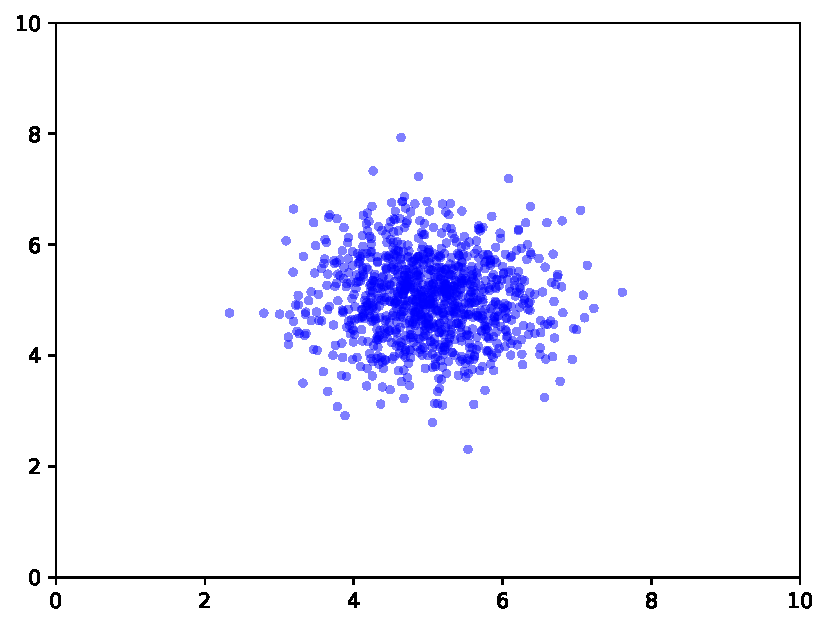
\includegraphics[width=0.19\linewidth]{figures/old/exp_multi_observation_base_N_3_gt_samples}
  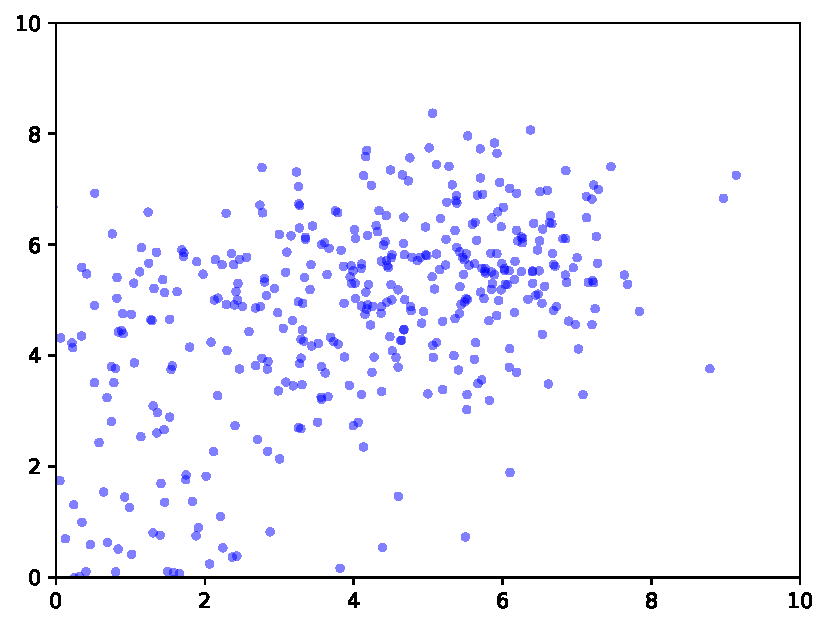
\includegraphics[width=0.19\linewidth]{figures/old/exp_multi_observation_base_N_3_npe_samples}
  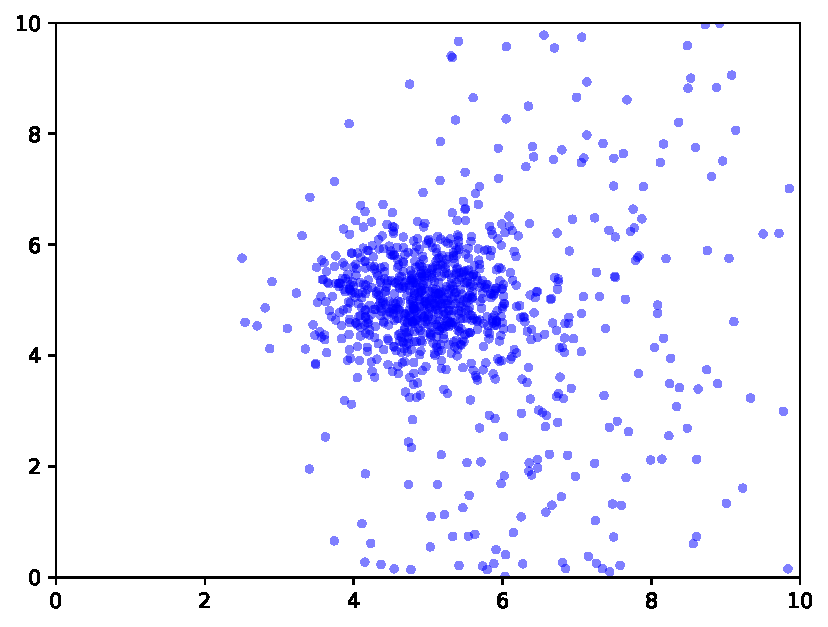
\includegraphics[width=0.19\linewidth]{figures/old/exp_multi_observation_base_N_3_nle_samples}
  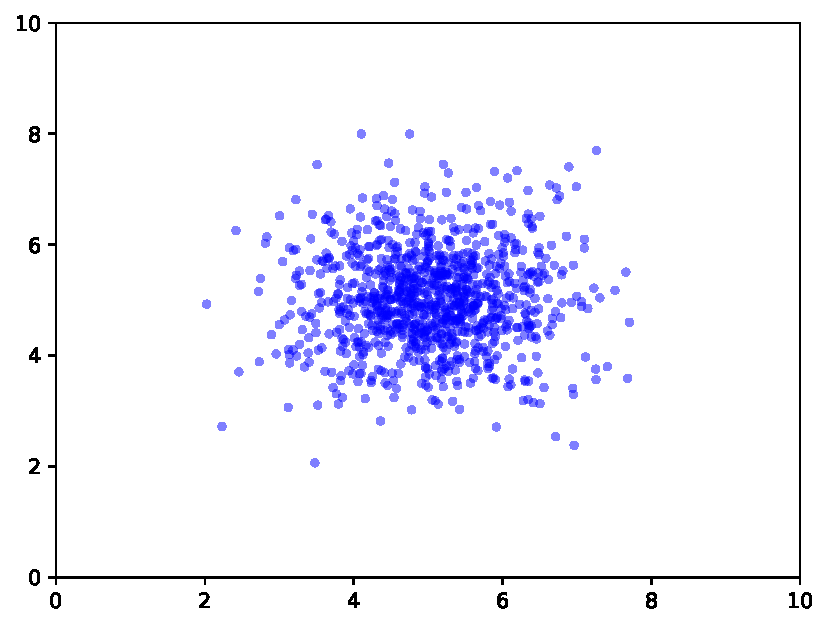
\includegraphics[width=0.19\linewidth]{figures/old/exp_multi_observation_base_N_3_romc_samples}
  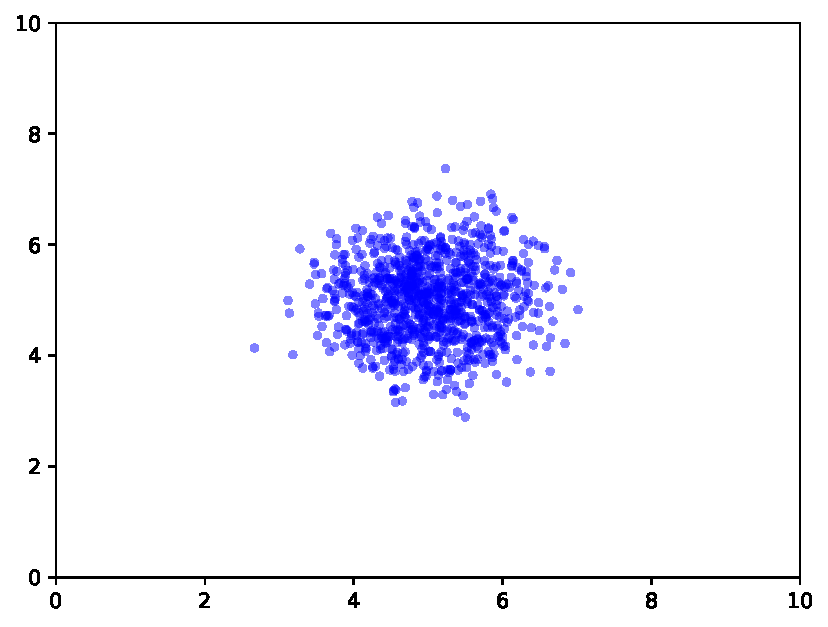
\includegraphics[width=0.19\linewidth]{figures/old/exp_multi_observation_base_N_3_r2omc_samples}\\
  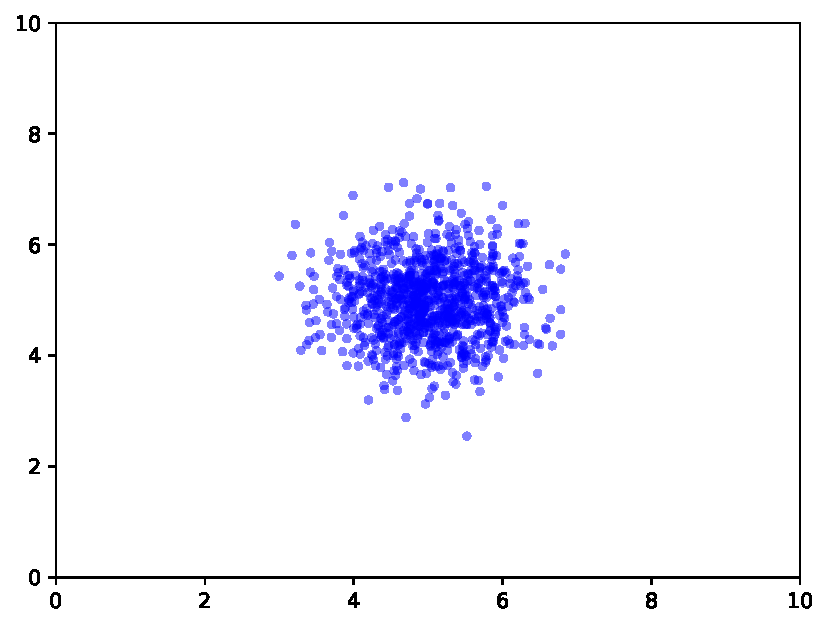
\includegraphics[width=0.19\linewidth]{figures/old/exp_multi_observation_base_N_5_gt_samples}
  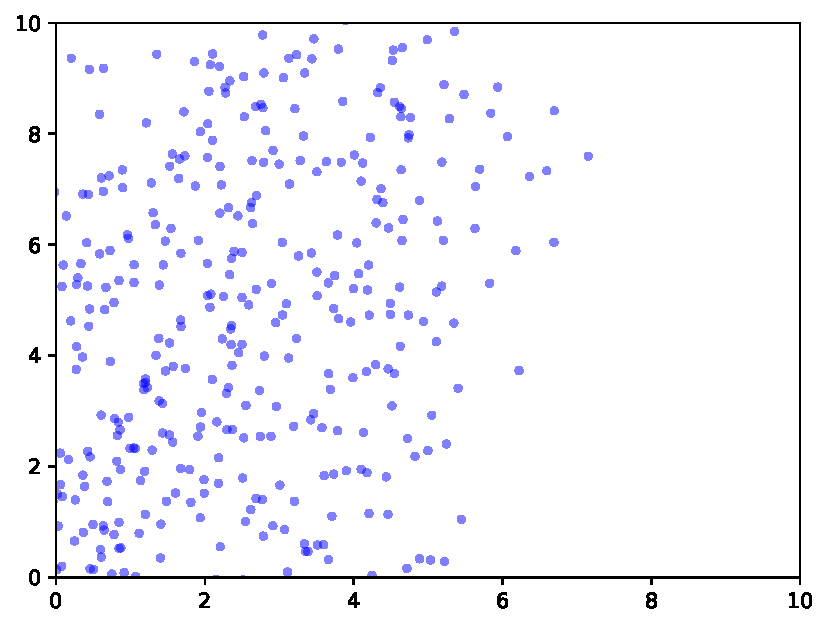
\includegraphics[width=0.19\linewidth]{figures/old/exp_multi_observation_base_N_5_npe_samples}
  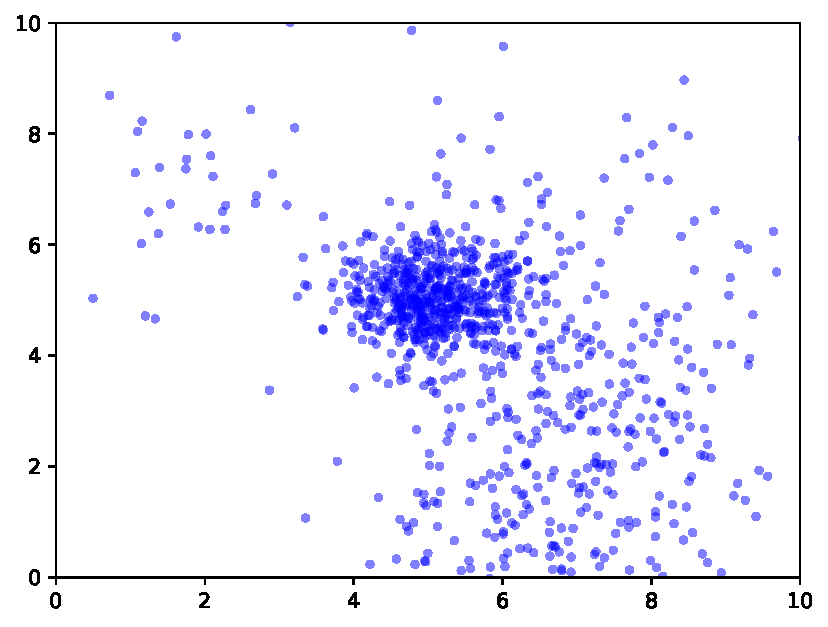
\includegraphics[width=0.19\linewidth]{figures/old/exp_multi_observation_base_N_5_nle_samples}
  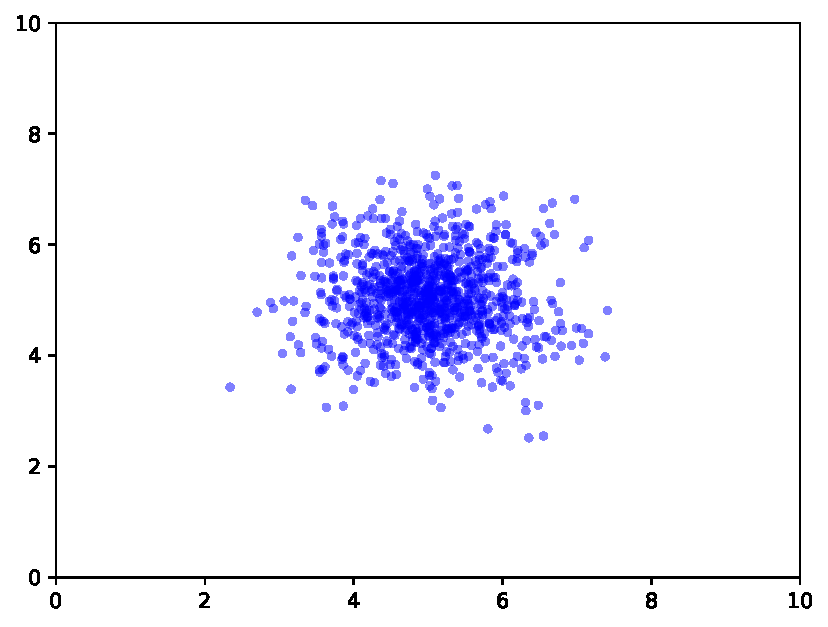
\includegraphics[width=0.19\linewidth]{figures/old/exp_multi_observation_base_N_5_romc_samples}
  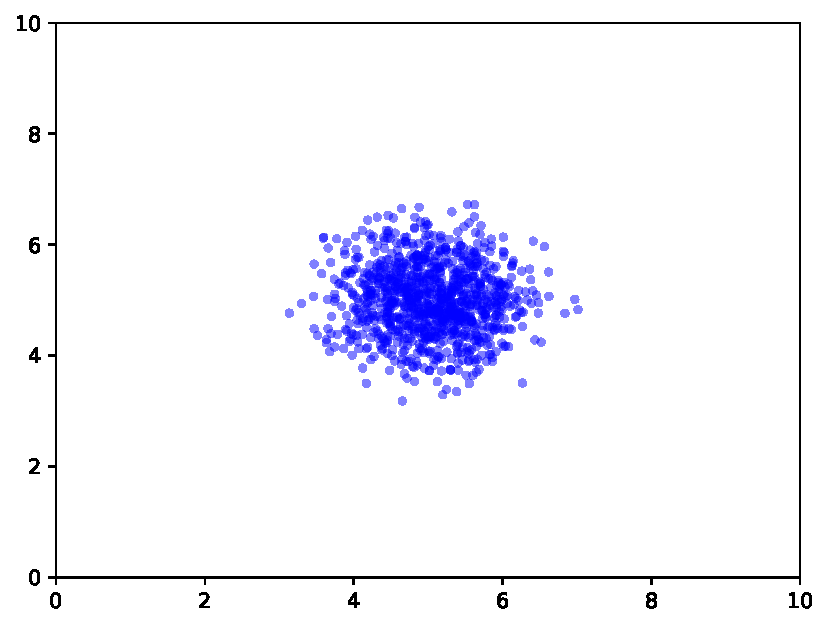
\includegraphics[width=0.19\linewidth]{figures/old/exp_multi_observation_base_N_5_r2omc_samples}\\
  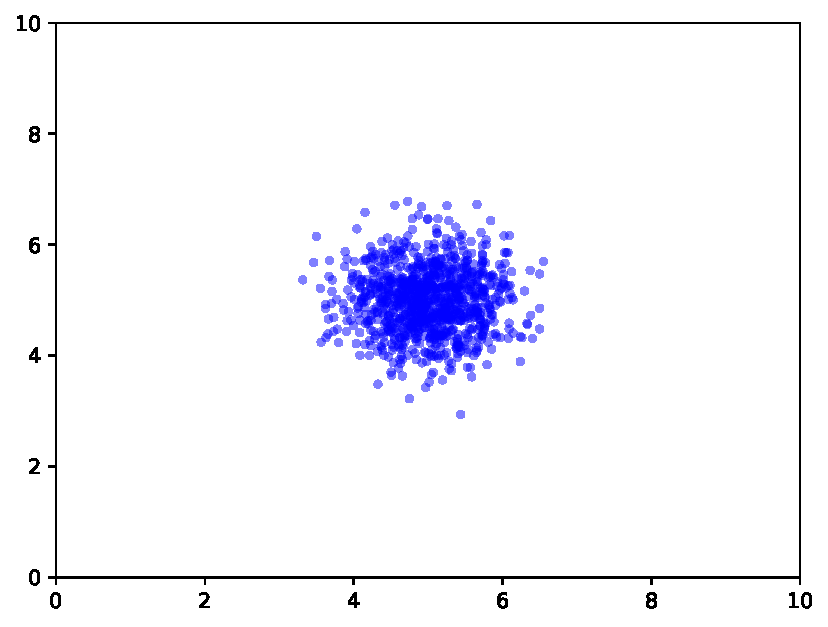
\includegraphics[width=0.19\linewidth]{figures/old/exp_multi_observation_base_N_10_gt_samples}
  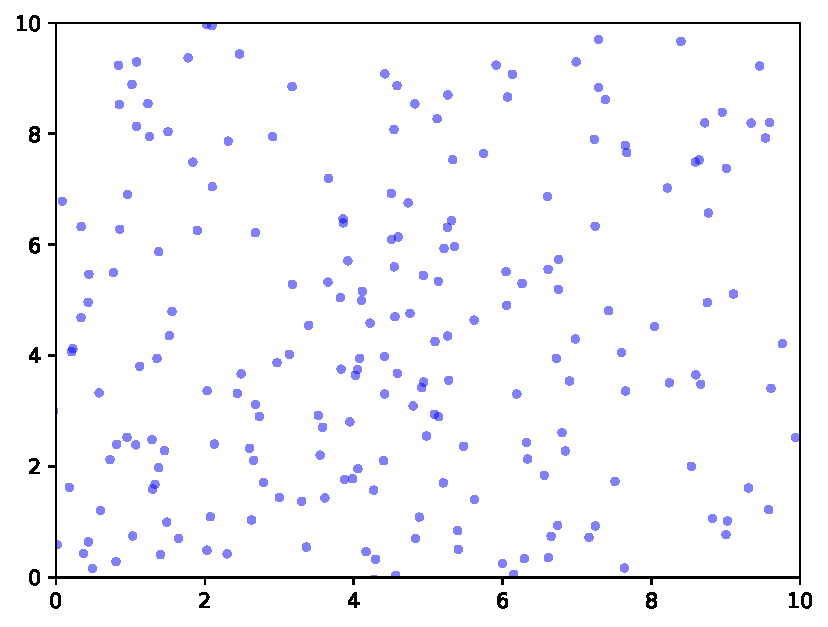
\includegraphics[width=0.19\linewidth]{figures/old/exp_multi_observation_base_N_10_npe_samples}
  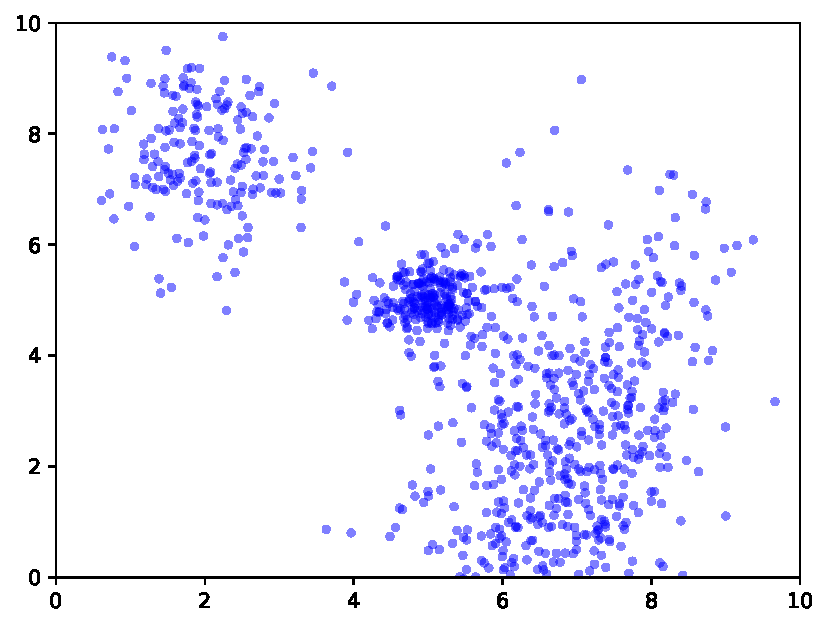
\includegraphics[width=0.19\linewidth]{figures/old/exp_multi_observation_base_N_10_nle_samples}
  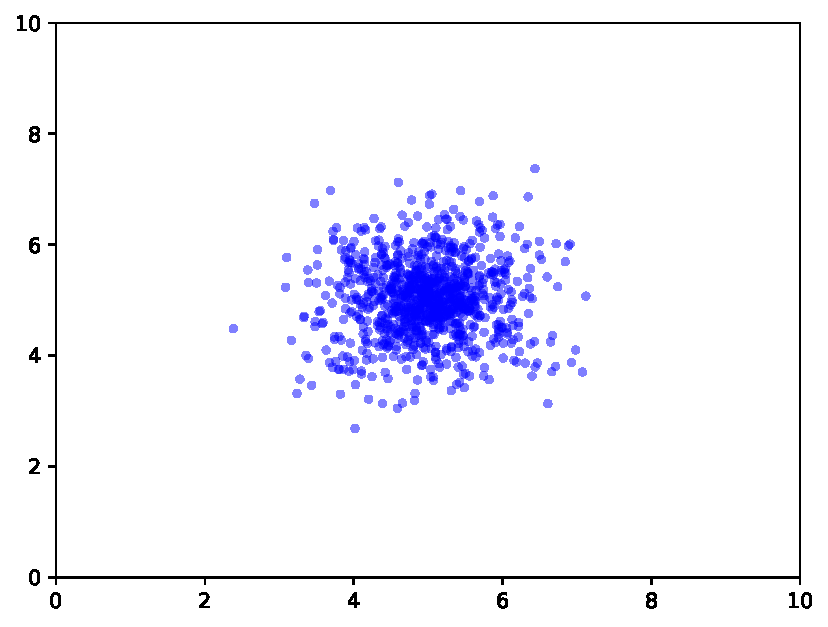
\includegraphics[width=0.19\linewidth]{figures/old/exp_multi_observation_base_N_10_romc_samples}
  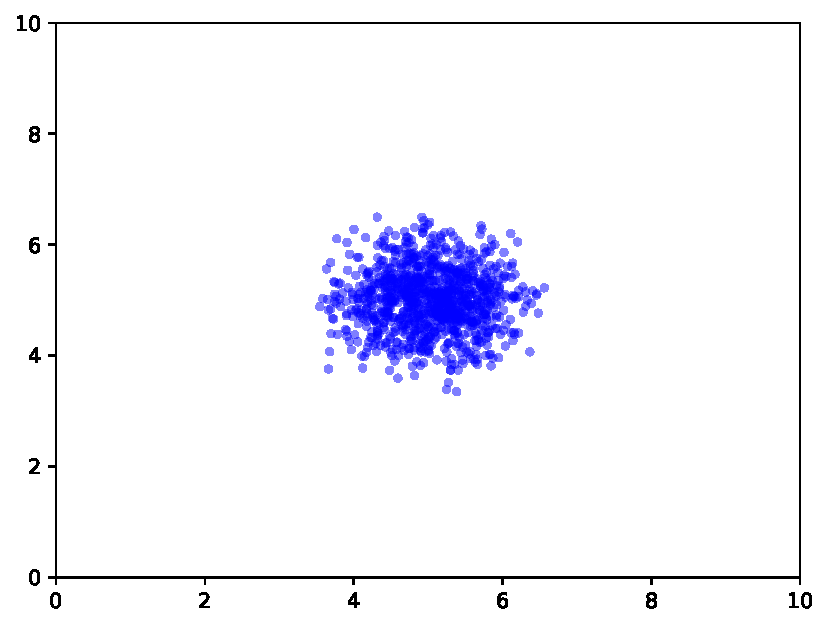
\includegraphics[width=0.19\linewidth]{figures/old/exp_multi_observation_base_N_10_r2omc_samples}\\
  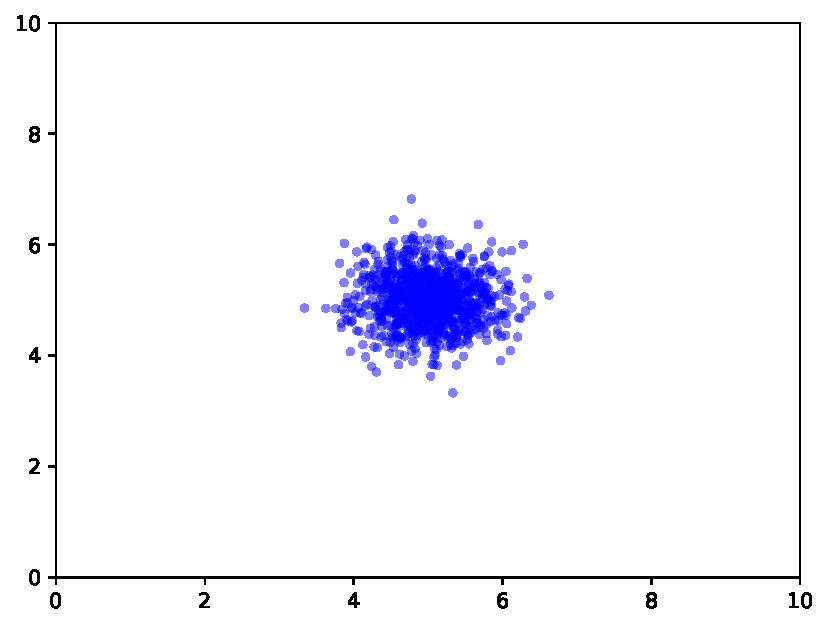
\includegraphics[width=0.19\linewidth]{figures/old/exp_multi_observation_base_N_20_gt_samples}
  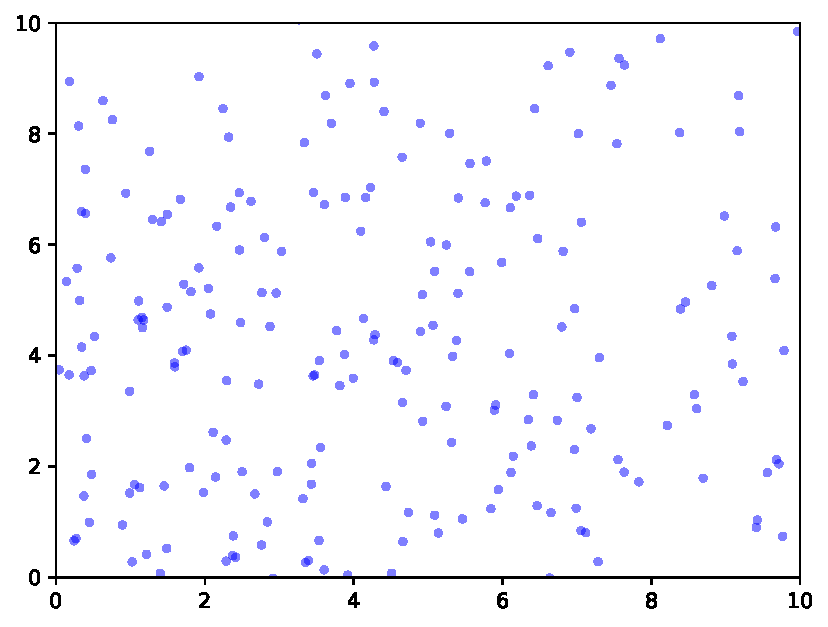
\includegraphics[width=0.19\linewidth]{figures/old/exp_multi_observation_base_N_20_npe_samples}
  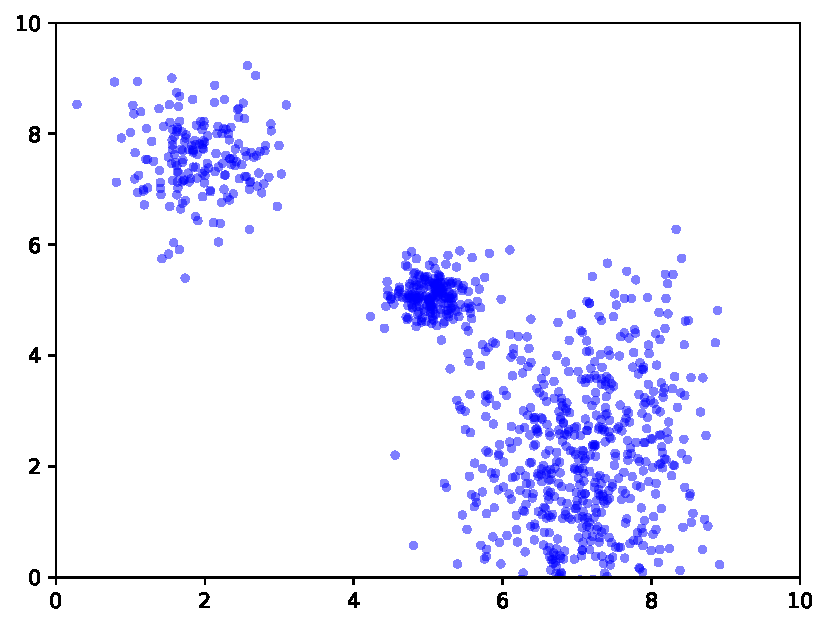
\includegraphics[width=0.19\linewidth]{figures/old/exp_multi_observation_base_N_20_nle_samples}
  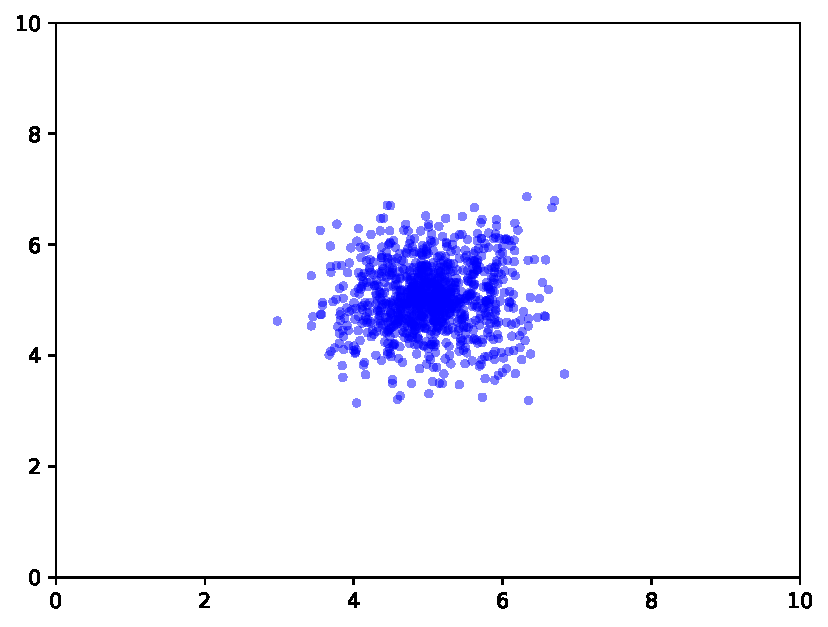
\includegraphics[width=0.19\linewidth]{figures/old/exp_multi_observation_base_N_20_romc_samples}
  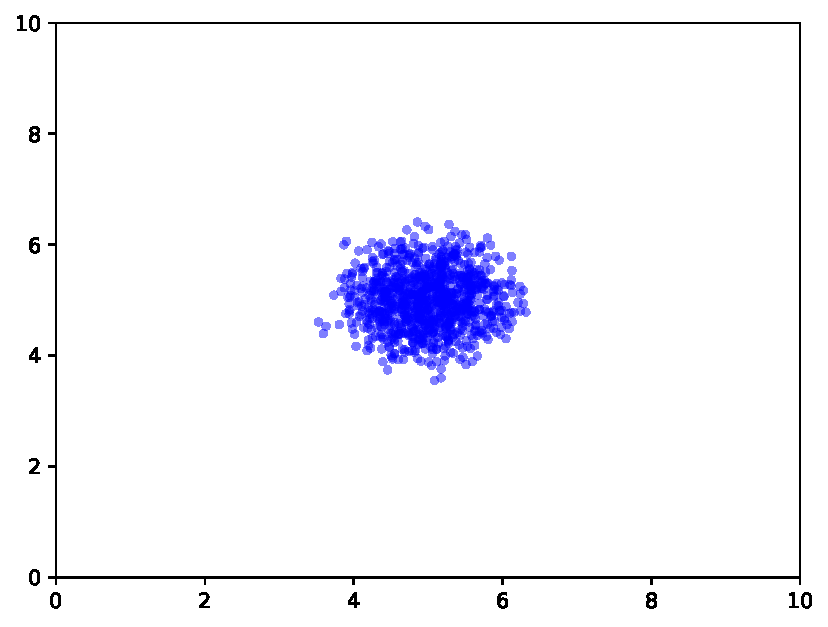
\includegraphics[width=0.19\linewidth]{figures/old/exp_multi_observation_base_N_20_r2omc_samples}
  \caption{Multi observations Base: Left to right: ground truth, NPE, NLE, Naive-ROMC, R2OMC. Top to bottom: $N=3$, $N=5$, $N=10$, $N=10$}
  \label{fig:mo_multi_obs_base}
\end{figure}


\subsubsection{MoG simulator}

\begin{tabular}{@{}ll@{}}
  \textbf{Prior} & $\thb \sim \mathcal{U}(-\mathbf{15}, \mathbf{15})$ \\ [5pt]
  \textbf{Simulator} & $\yb \sim \frac{1}{2} \left( \mathcal{N}(\thb, \sigma_1^2 \mathbf{I}) + \mathcal{N}(-\thb, \sigma_2^2 \mathbf{I}) \right)$, with $\sigma_1=\sigma_2=1$ \\ [5pt]
  \textbf{Dimensionality} & $\thb \in \mathbb{R}^{D}$, $\yb \in \mathbb{R}^{D}$ \\ [5pt]
  \textbf{Observations} & $\{\data_n\}_n^N$ where: \\ [5pt]
  & $\data_n = (5, \ldots, 5) + \epsilon$ for $n \in \{1, \ldots, \frac{N}{2}\}$, \\ [5pt] 
  & $\data_n = (-5, \ldots, -5) + \epsilon$ for $n \in \{\frac{N}{2}+1, \ldots, N\}$ \\ [5pt]
  \textbf{Posterior} & $ p(\thb | \data) \propto
                                    \begin{cases}
                                      \mathcal{N}(\thb; \mathbf{5}, \frac{1}{N} \mathbf{I}) + \mathcal{N}(\thb; -\mathbf{5}, \frac{1}{N} \mathbf{I}), & \text{if } \thb \in [-15, 15]^D, \\
                                      0, & \text{otherwise}.
                                    \end{cases} $ \\ [5pt]
\end{tabular}

\textbf{Proof of the posterior:}
\begin{equation}
  p(\thb|\{\data_n\}) \appropto 
  \begin{cases}
    \mathcal{N}(\thb; \mathbf{5}, \frac{1}{N} \mathbf{I}) + \mathcal{N}(\thb; -\mathbf{5}, \frac{1}{N}\mathbf{I}), & \text{if } \thb \in [-15, 15]^D, \\
    0, & \text{otherwise}.
  \end{cases}
  \label{eq:mog_mog_mult_obs}
\end{equation}
The proof is similar to the one in Eq.~(\ref{eq:intro-multiple}).

In Figure~\ref{fig:mog_multi_obs}, we present the results for the MoG simulator with multiple observations.


\begin{figure}[]
  \centering
  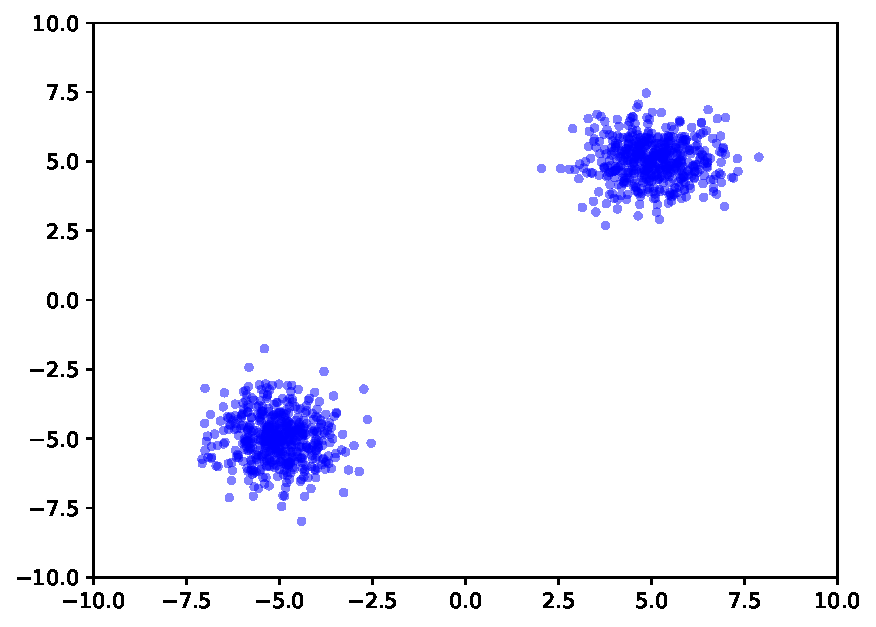
\includegraphics[width=0.19\linewidth]{figures/old/exp_multi_observation_MoG_N_2_gt_samples}
  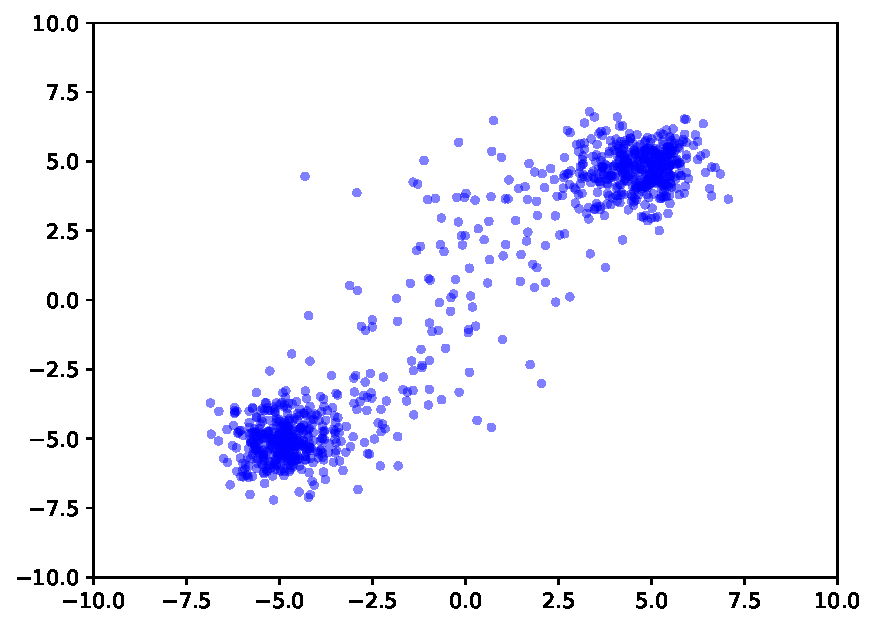
\includegraphics[width=0.19\linewidth]{figures/old/exp_multi_observation_MoG_N_2_npe_samples}
  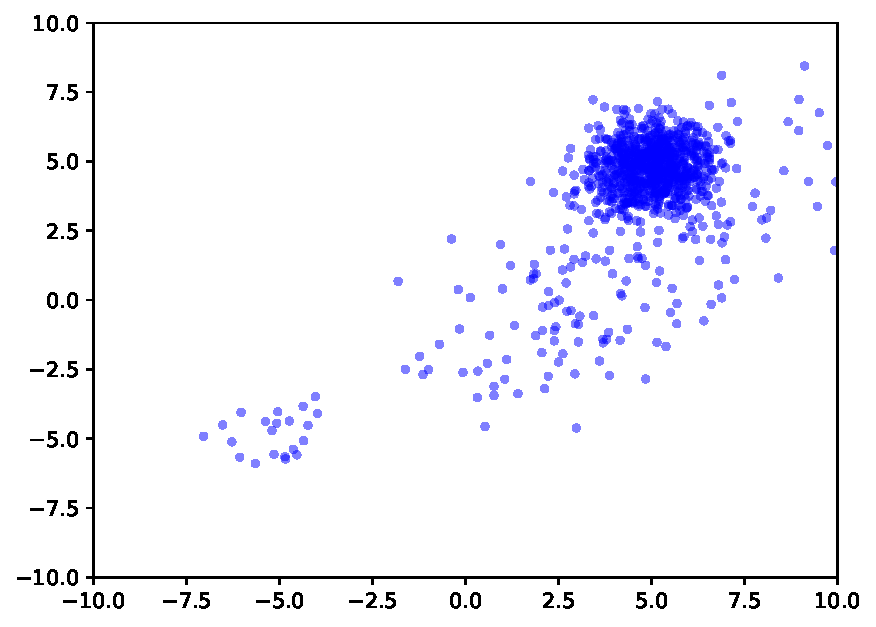
\includegraphics[width=0.19\linewidth]{figures/old/exp_multi_observation_MoG_N_2_nle_samples}
  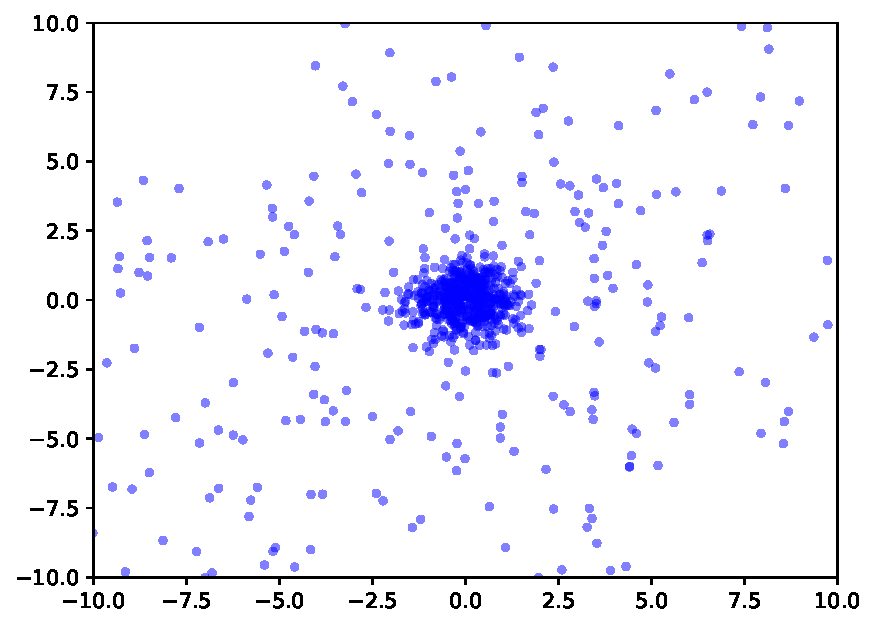
\includegraphics[width=0.19\linewidth]{figures/old/exp_multi_observation_MoG_N_2_romc_samples}
  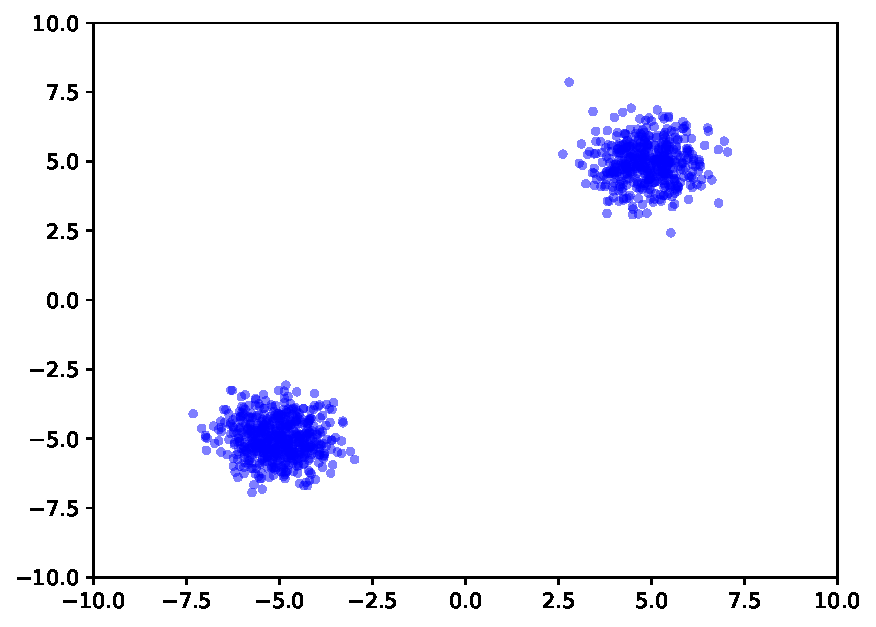
\includegraphics[width=0.19\linewidth]{figures/old/exp_multi_observation_MoG_N_2_r2omc_samples}\\
  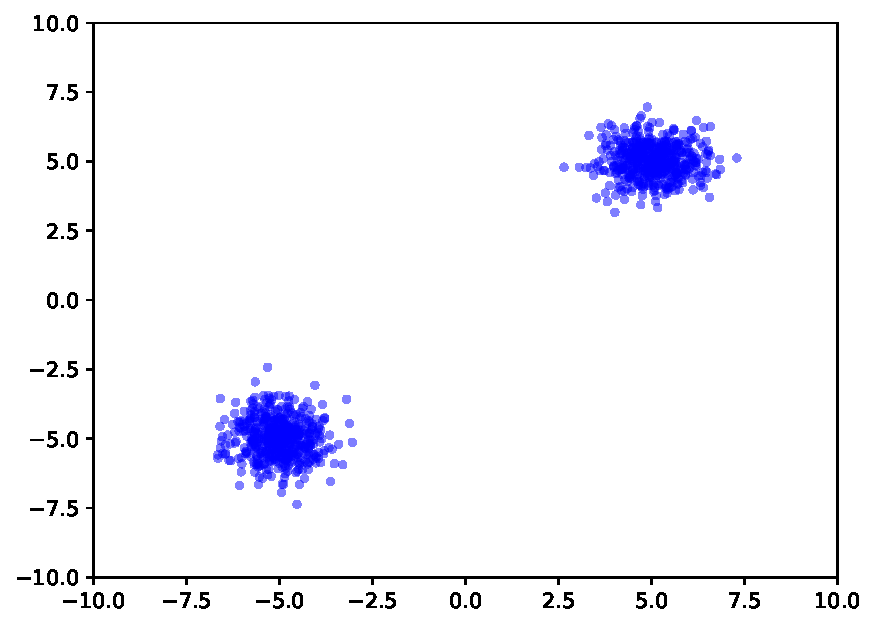
\includegraphics[width=0.19\linewidth]{figures/old/exp_multi_observation_MoG_N_5_gt_samples}
  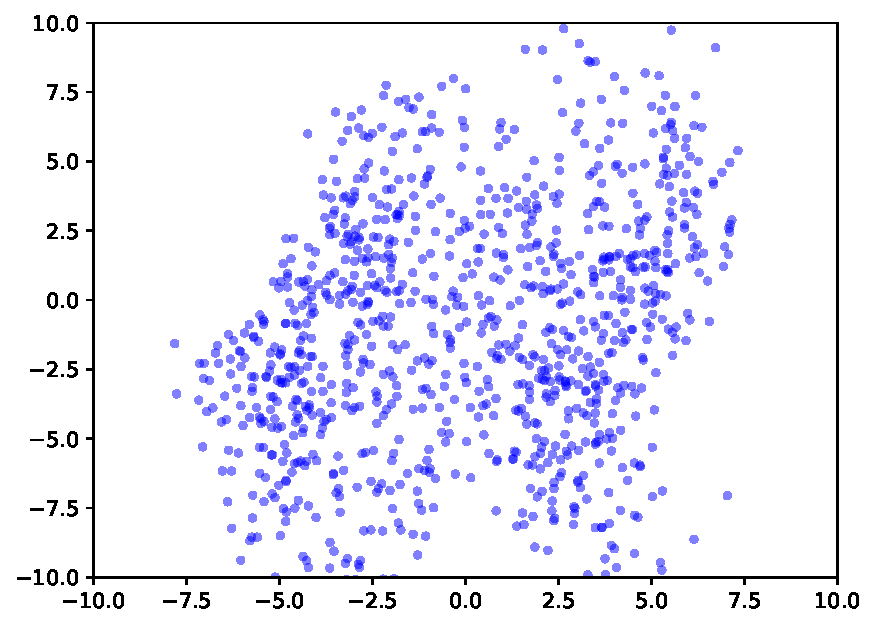
\includegraphics[width=0.19\linewidth]{figures/old/exp_multi_observation_MoG_N_5_npe_samples}
  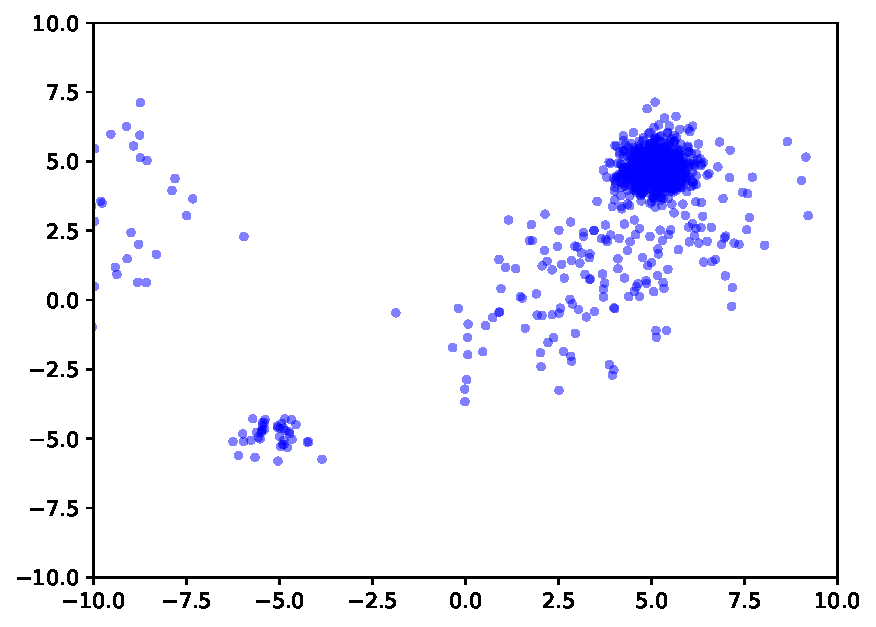
\includegraphics[width=0.19\linewidth]{figures/old/exp_multi_observation_MoG_N_5_nle_samples}
  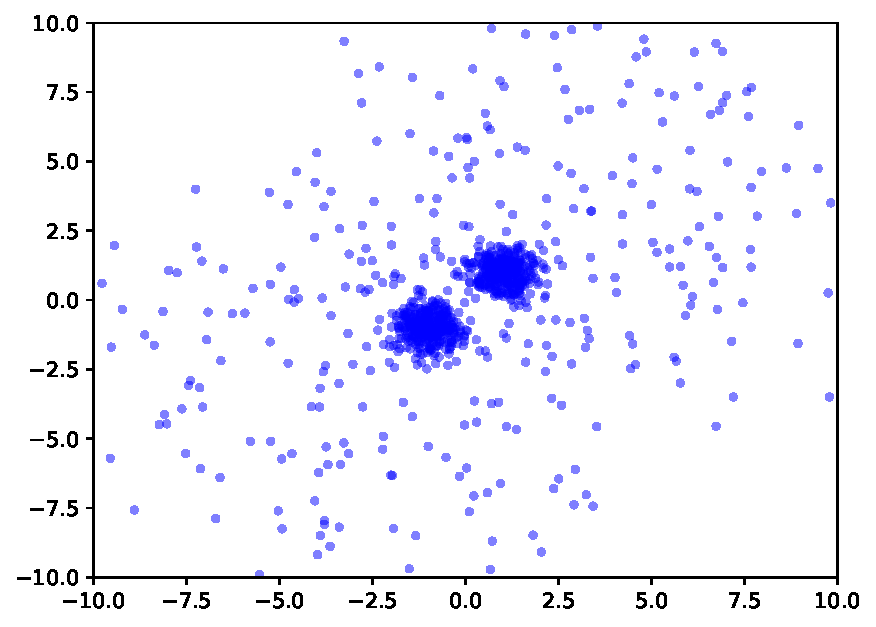
\includegraphics[width=0.19\linewidth]{figures/old/exp_multi_observation_MoG_N_5_romc_samples}
  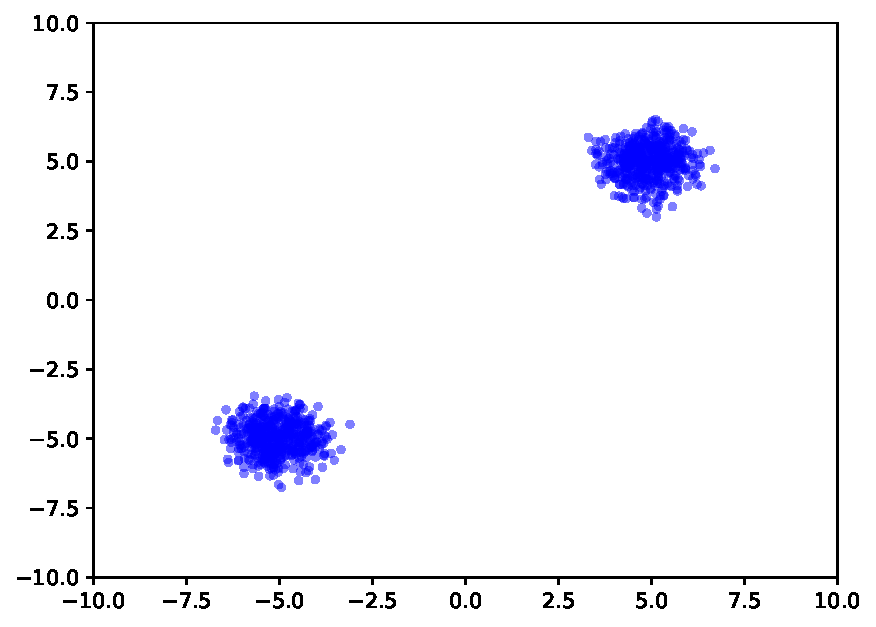
\includegraphics[width=0.19\linewidth]{figures/old/exp_multi_observation_MoG_N_5_r2omc_samples}\\
  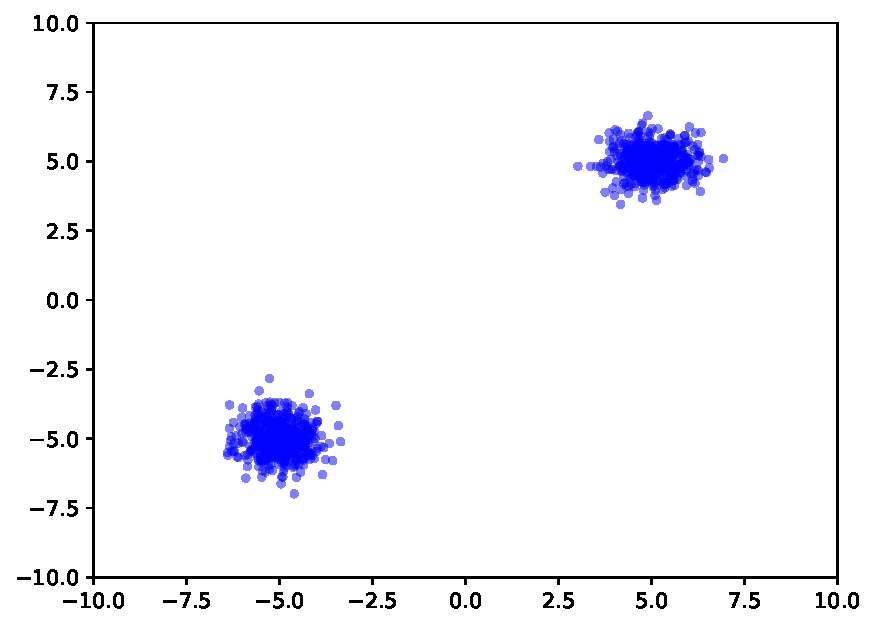
\includegraphics[width=0.19\linewidth]{figures/old/exp_multi_observation_MoG_N_10_gt_samples}
  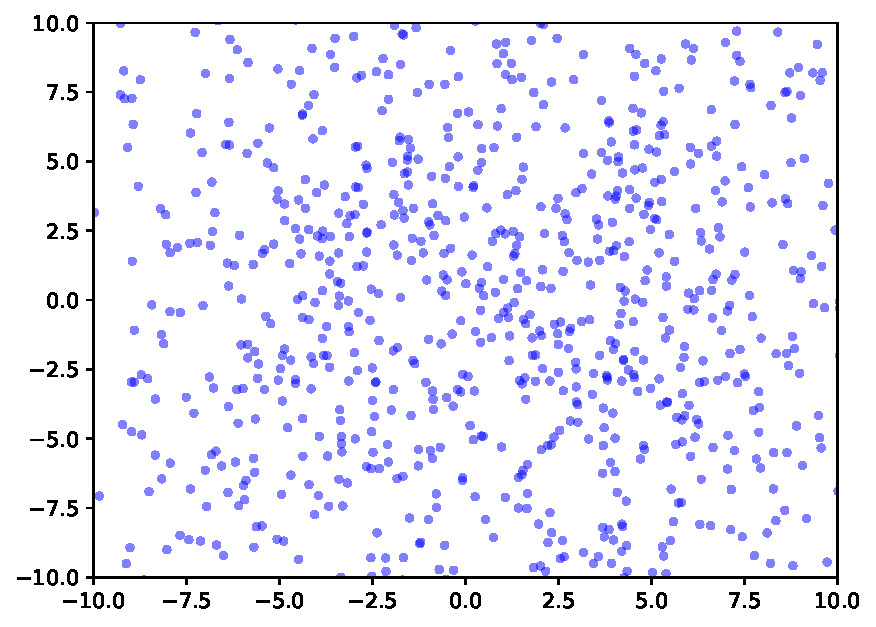
\includegraphics[width=0.19\linewidth]{figures/old/exp_multi_observation_MoG_N_10_npe_samples}
  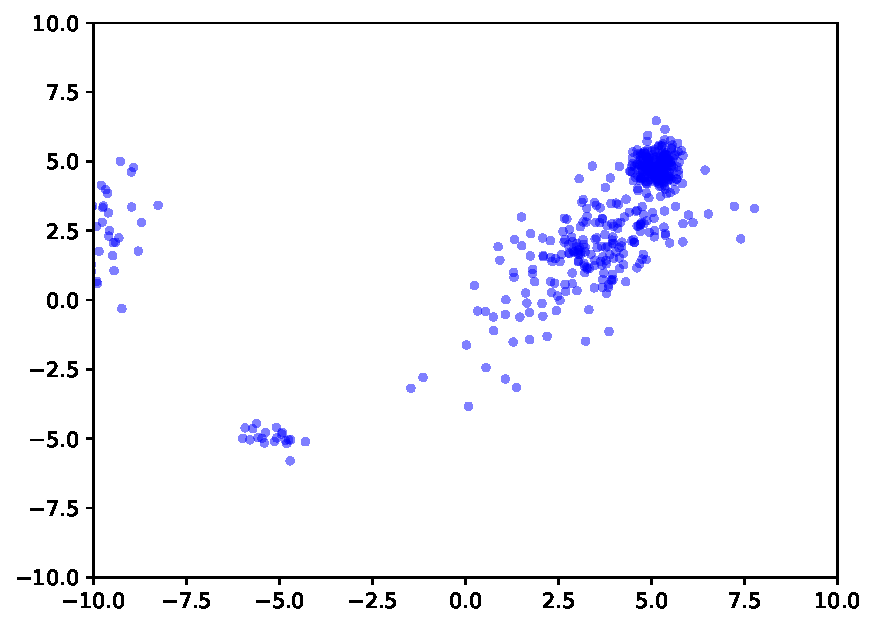
\includegraphics[width=0.19\linewidth]{figures/old/exp_multi_observation_MoG_N_10_nle_samples}
  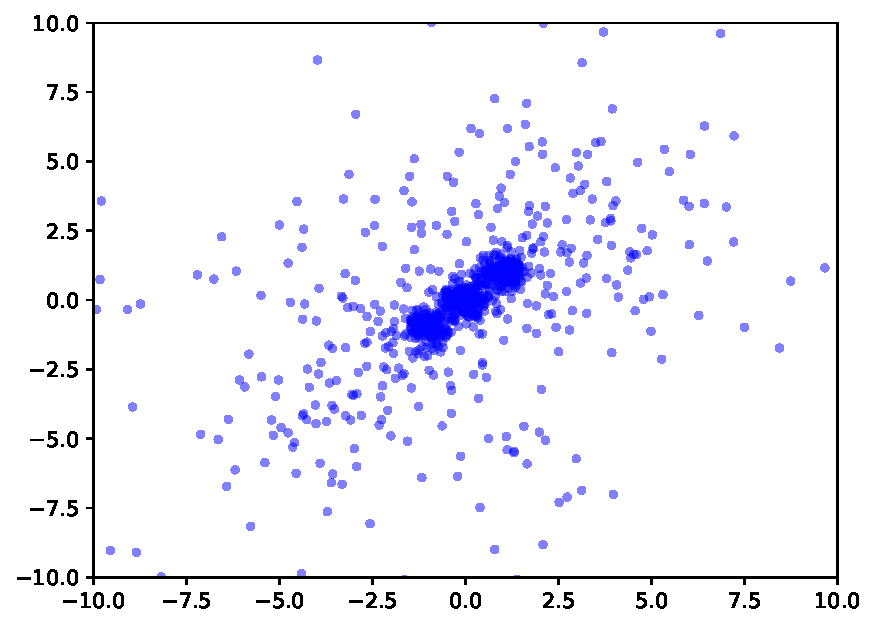
\includegraphics[width=0.19\linewidth]{figures/old/exp_multi_observation_MoG_N_10_romc_samples}
  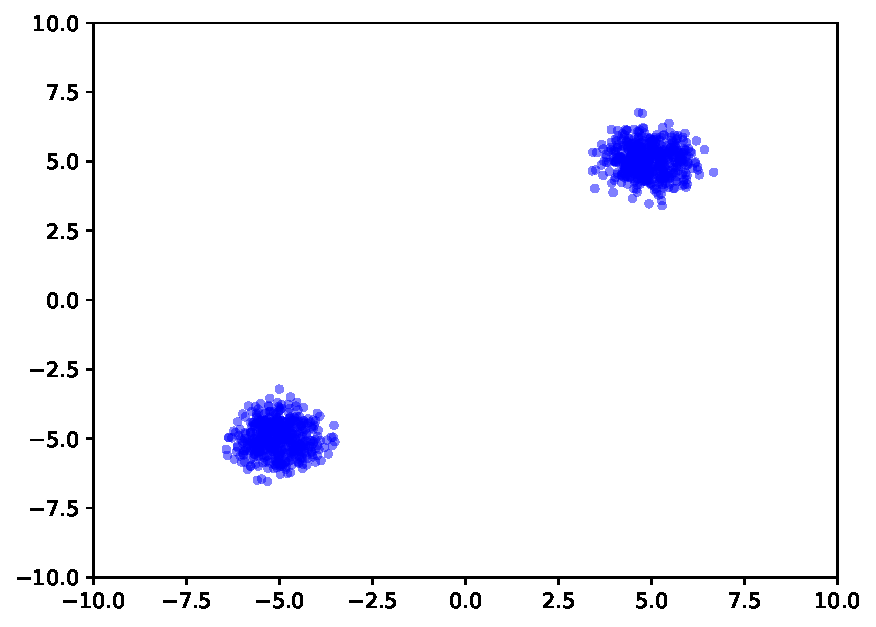
\includegraphics[width=0.19\linewidth]{figures/old/exp_multi_observation_MoG_N_10_r2omc_samples}\\
  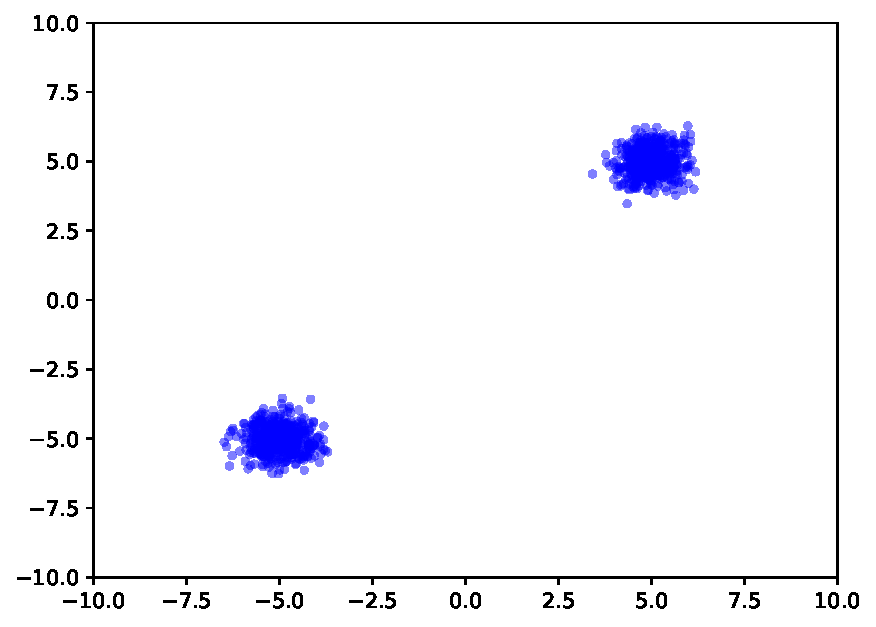
\includegraphics[width=0.19\linewidth]{figures/old/exp_multi_observation_MoG_N_20_gt_samples}
  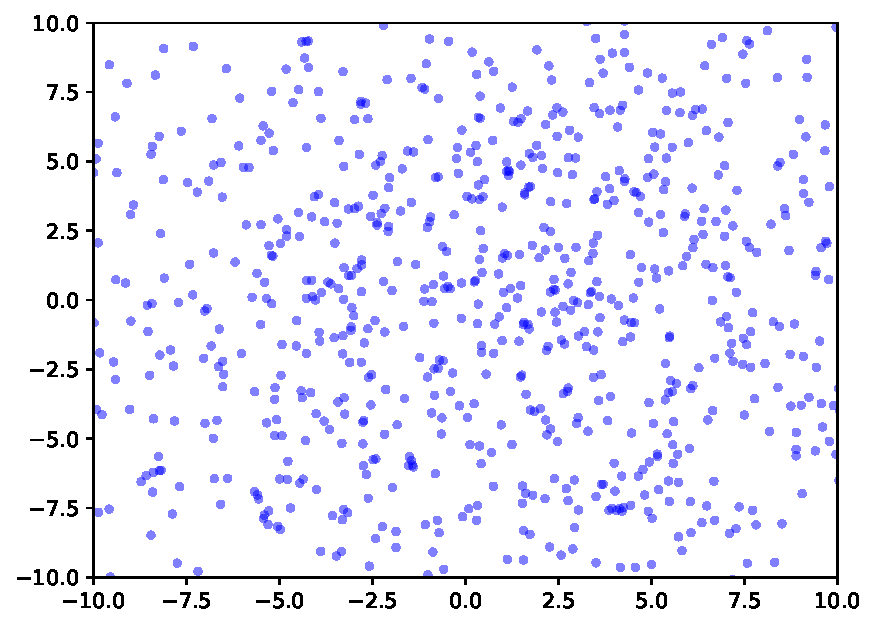
\includegraphics[width=0.19\linewidth]{figures/old/exp_multi_observation_MoG_N_20_npe_samples}
  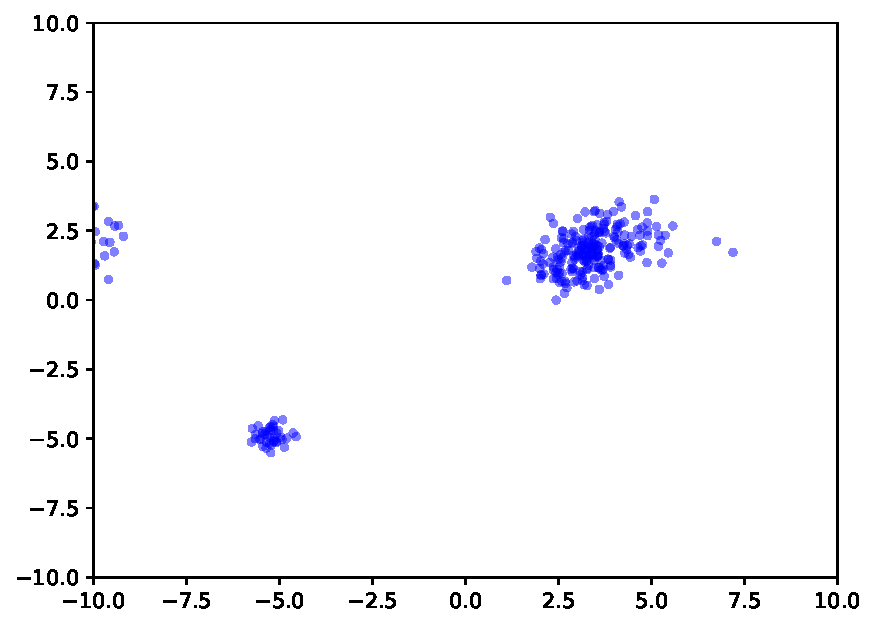
\includegraphics[width=0.19\linewidth]{figures/old/exp_multi_observation_MoG_N_20_nle_samples}
  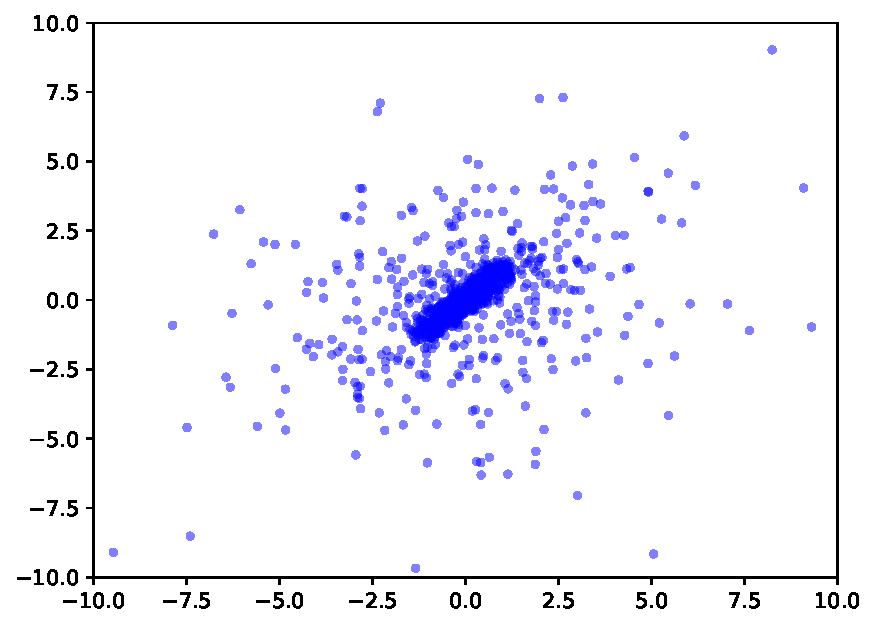
\includegraphics[width=0.19\linewidth]{figures/old/exp_multi_observation_MoG_N_20_romc_samples}
  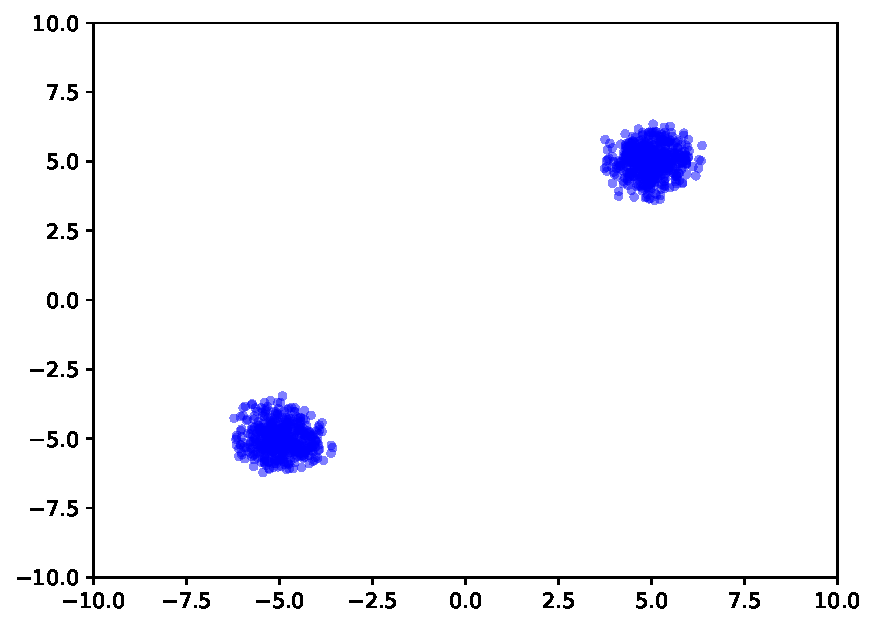
\includegraphics[width=0.19\linewidth]{figures/old/exp_multi_observation_MoG_N_20_r2omc_samples}
  \caption{Multi observations MoG: Left to right: ground truth, NPE, NLE, Naive-ROMC, R2OMC. Top to bottom: $N=3$, $N=5$, $N=10$, $N=10$}
  \label{fig:mog_multi_obs}
\end{figure}

\subsection{SBI - Mixtures of Gaussians (T.7)}

We here provide additional information on example T.7 of the SBI benchmark~\cite{lueckmann2021benchmarking}.
It tests inference of the mean of a mixture of two $2$-D Gaussians, one with much broader covariance than the other

\begin{tabular}{@{}ll@{}}
  \textbf{Prior} & $\thb \sim \mathcal{U}(-\mathbf{10}, \mathbf{10})$ \\ [5pt]
  \textbf{Simulator} & $\yb \sim 0.5 (\mathcal{N}(\thb, \mathbf{I}) + \mathcal{N}(\thb, \sigma^2 \mathbf{I}))$, with $\sigma^2 = 0.01$ \\ [5pt]
  \textbf{Dimensionality} & $\thb \in \mathbb{R}^{2}$, $\yb \in \mathbb{R}^{2}$ \\ [5pt]
\end{tabular}

\paragraph{Results.}

We evaluate \rromc~using a simulation budget of $S=1000$ and $S=10000$ seeds.
The \texttt{C2ST} score is computed by comparing 1000 samples from the true posterior (we randomly select 1000 from the 10000 that are provided by the SBI benchmark)
with 1000 samples generated from the \rromc~approximate posterior.
The results are illustrated in Figure~\ref{fig:exp_sbi_gaussian_mixture}.

\begin{figure}[ht]
  \centering
  \begin{subfigure}[b]{0.32\linewidth}
    \centering
    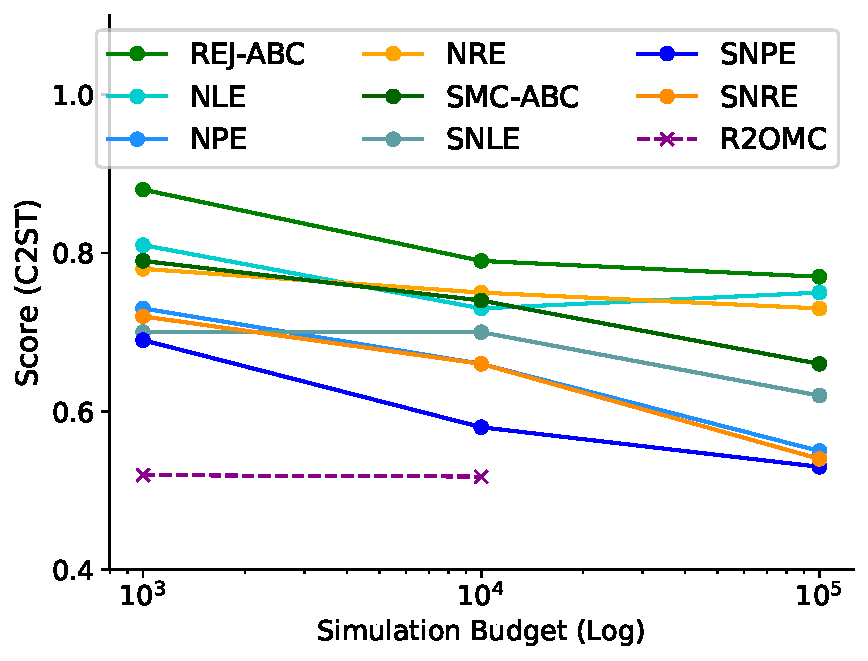
\includegraphics[width=\linewidth]{figures/old/gaussian_mixture}
    \caption{\texttt{C2ST} score}
  \end{subfigure}
  \hfill
  \begin{subfigure}[b]{0.32\linewidth}
    \centering
    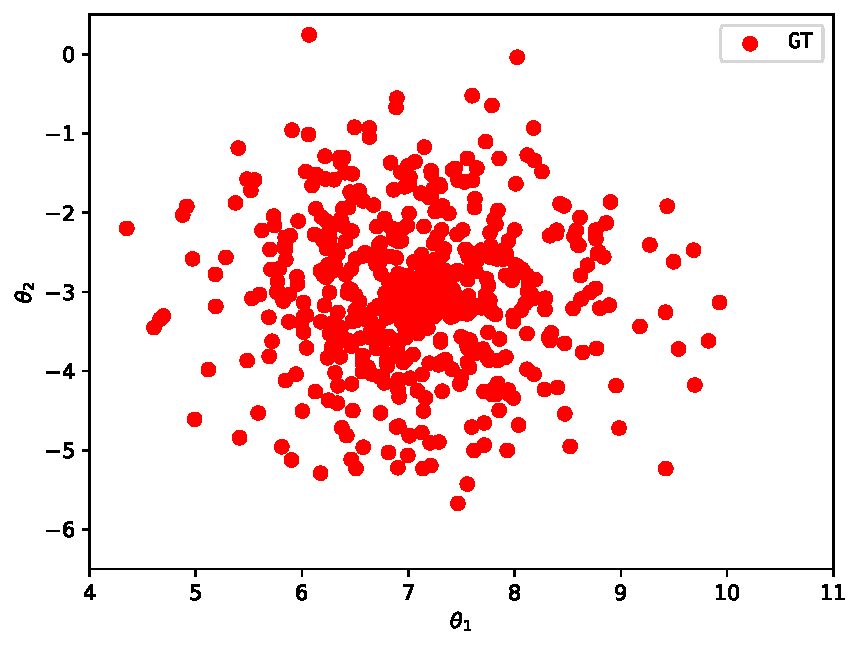
\includegraphics[width=\linewidth]{figures/old/exp_sbi_gaussian_mixture_gt}
    \caption{Ground truth samples}
  \end{subfigure}
  \hfill
  \begin{subfigure}[b]{0.32\linewidth}
    \centering
    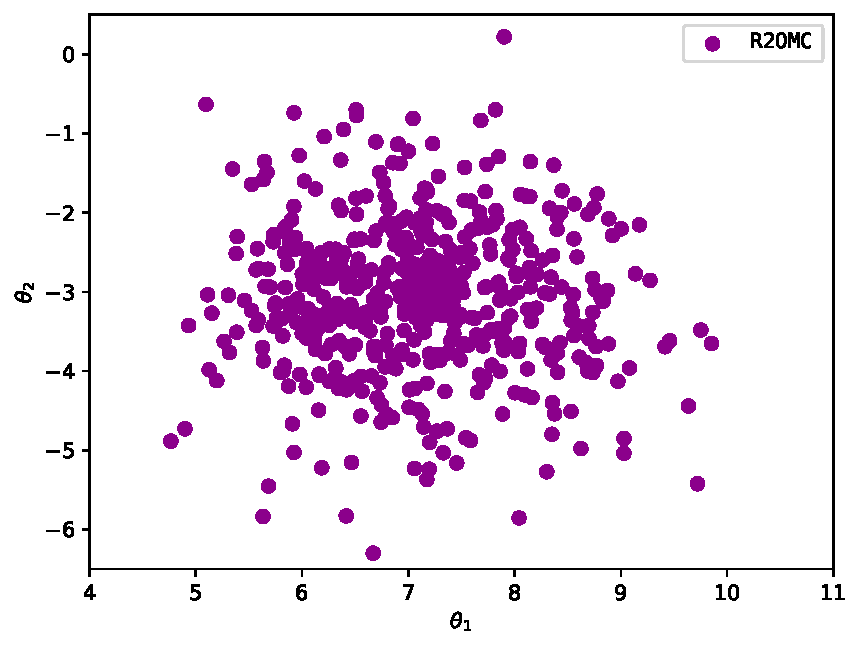
\includegraphics[width=\linewidth]{figures/old/exp_sbi_gaussian_mixture_r2omc}
    \caption{Samples by R2OMC}
  \end{subfigure}
  \caption{T.7: Gaussian Mixture. From left to right: \texttt{C2ST} score, ground truth samples, and samples by R2OMC.}
  \label{fig:exp_sbi_gaussian_mixture}
\end{figure}

\subsection{SBI - Two Moons (T.8)}

We here provide additional information on example T.8 of the SBI benchmark~\cite{lueckmann2021benchmarking}.
It tests inference when the posterior exhibits both global (bimodality) and local (crescent shape) structure to illustrate how algorithms deal with multimodality:

\begin{tabular}{@{}ll@{}}
  \textbf{Prior} & $\thb \sim \mathcal{U}(-\mathbf{1}, \mathbf{1})$ \\ [5pt]
  \textbf{Simulator} & $\yb \sim \begin{bmatrix} 
    r \cos(\alpha) + 0.25 \\ 
    r \sin(\alpha)
  \end{bmatrix} + \begin{bmatrix} 
    |\theta_1 + \theta_2|/\sqrt{2} \\ 
    (-\theta_1 + \theta_2)/\sqrt{2}
  \end{bmatrix}$, where $r \sim \mathcal{N}(0.1, 0.01^2)$ and $\alpha \sim \mathcal{U}(-\pi/2, \pi/2)$ \\ [10pt]
  \textbf{Dimensionality} & $\thb \in \mathbb{R}^{2}$, $\yb \in \mathbb{R}^{2}$ \\ [5pt]
\end{tabular}

\paragraph{Results.}

We evaluate \rromc~using a simulation budget of $S=1000$ and $S=10000$ seeds.
The \texttt{C2ST} score is computed by comparing 1000 samples from the true posterior (we randomly select 1000 from the 10000 that are provided by the SBI benchmark)
with 1000 samples generated from the \rromc~approximate posterior.
The results are illustrated in Figure~\ref{fig:exp_sbi_gaussian_mixture}.
We observe that \rromc~is able to capture the bimodal structure of the posterior, perfectly replicating the ground truth samples.

\begin{figure}[ht]
  \centering
  \begin{subfigure}[b]{0.32\linewidth}
    \centering
    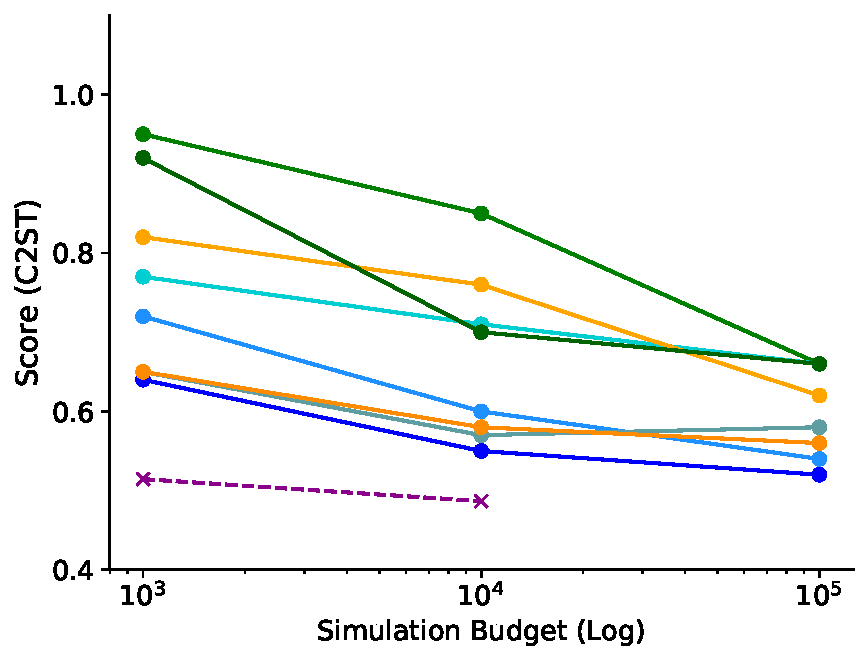
\includegraphics[width=\linewidth]{figures/old/two_moons}
    \caption{\texttt{C2ST} score}
  \end{subfigure}
  \hfill
  \begin{subfigure}[b]{0.32\linewidth}
    \centering
    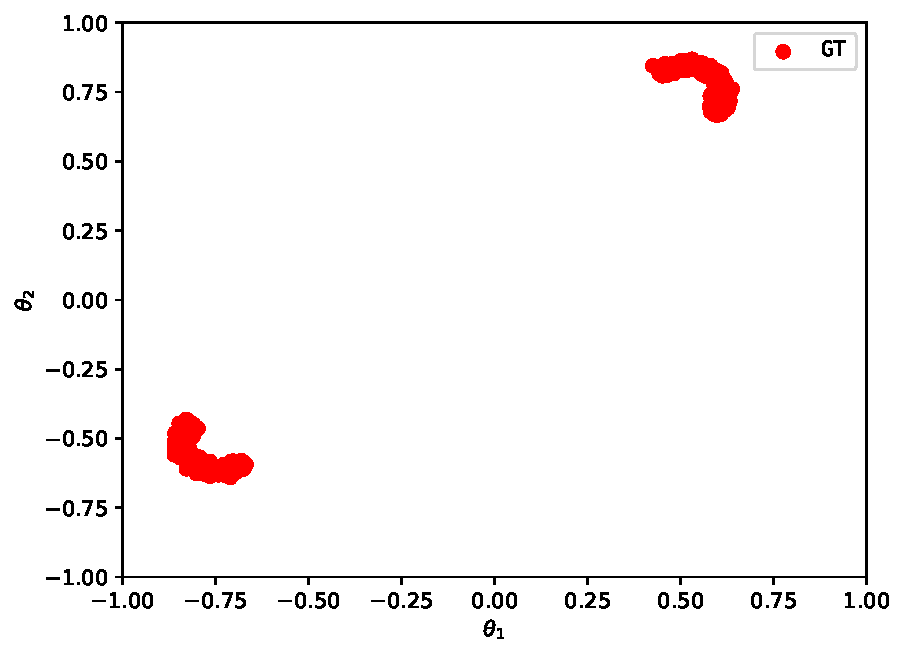
\includegraphics[width=\linewidth]{figures/old/exp_sbi_two_moons_gt}
    \caption{Ground truth samples}
  \end{subfigure}
  \hfill
  \begin{subfigure}[b]{0.32\linewidth}
    \centering
    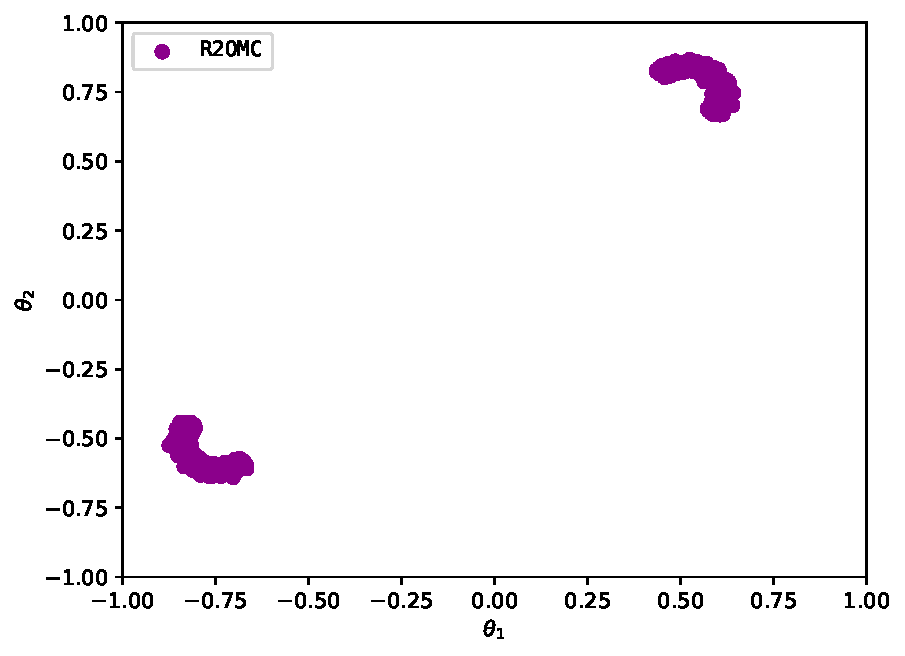
\includegraphics[width=\linewidth]{figures/old/exp_sbi_two_moons_r2omc}
    \caption{Samples by R2OMC}
  \end{subfigure}
  \caption{T.8: Two Moons. From left to right: \texttt{C2ST} score, ground truth samples, and samples by R2OMC.}
  \label{fig:exp_sbi_two_moons}
\end{figure}

\clearpage

\section{Additional results}
\label{sec:additional-experiments}

We here present some additional experiments that were not included in the main text.

% \subsection{SBI - Gaussian Linear Uniform (T.2)}

% This is the T.2 from the SBI benchmark~\cite{lueckmann2021benchmarking}.
% It tests inference of the mean of a $10$-D Gaussian model with fixed covariance.
% The posterior is a truncated Gaussian distribution:

% \begin{tabular}{@{}ll@{}}
%   \textbf{Prior} & $\thb \sim \mathcal{U}(-1, 1)$ \\[5pt]
%   \textbf{Simulator} & $\yb \sim \mathcal{N}(\thb, 0.1 \odot \mathbf{I})$ \\[5pt]
%   \textbf{Dimensionality} & $\thb \in \mathbb{R}^{10}$, $\yb \in \mathbb{R}^{10}$ \\[5pt]
% \end{tabular}

% \paragraph{Results.}

% We evaluate \rromc~using a simulation budget of $S=1000$ and $S=10000$ seeds.
% Running it for $S=100000$ seeds is omitted, as the \texttt{C2ST} score is almost $0.5$ (perfect score), even with just $S=1000$ seeds.
% The \texttt{C2ST} score is computed by comparing 1000 samples from the true posterior (we randomly select 1000 from the 10000 that are provided by the SBI benchmark)
% with 1000 samples generated from the \rromc~approximate posterior.
% The results are illustrated in Figure~\ref{fig:exp_sbi_extra} (Left).

% \subsection{SBI - SLCP (T.3)}

% This is the T.3 from the SBI benchmark~\cite{lueckmann2021benchmarking}.
% It is a challenging inference task designed to have a simple likelihood but a complex posterior.
% The prior is uniform over five parameters $\thb$ and the observations are four two-dimensional points sampled from a Gaussian likelihood
% whose mean and variance are nonlinear functions of $\thb$.

%\begin{tabular}{@{}ll@{}}
%   \textbf{Prior} & $\thb \sim \mathcal{U}(-3, 3)^5$ \\[5pt]
%   \textbf{Simulator} & $\mathbf{y} | \boldsymbol{\theta} \sim \mathcal{N}(\mathbf{m_{\theta}}, \mathbf{S_{\theta}}), \quad
%                        \mathbf{m_{\theta}} = \begin{bmatrix} \theta_1 \\ \theta_2 \end{bmatrix}, \quad
%                        \mathbf{S_{\theta}} = \begin{bmatrix} s_1^2 & \rho s_1 s_2 \\ \rho s_1 s_2 & s_2^2 \end{bmatrix},
%                        s_1 = \theta_3^2, s_2 = \theta_4^2, \rho = \tanh(\theta_5)$ \\[5pt]
%   \textbf{Dimensionality} & $\thb \in \mathbb{R}^{5}$, $\data_n \in \mathbb{R}^{2} \text{ for } n \in \{1, \ldots, 4\}$ \\[5pt] 
% \end{tabular}

% \paragraph{Results.}

% We evaluate \rromc~using a simulation budget of $S= \{1000, 10000, 100000\}$ seeds.
% The \texttt{C2ST} score is computed by comparing 1000 samples from the true posterior (we randomly select 1000 from the 10000 that are provided by the SBI benchmark)
% with 1000 samples generated from the \rromc~approximate posterior.
% The results are illustrated in Figure~\ref{fig:exp_sbi_extra}(Right).

% \begin{figure}[ht]
%   \centering
%   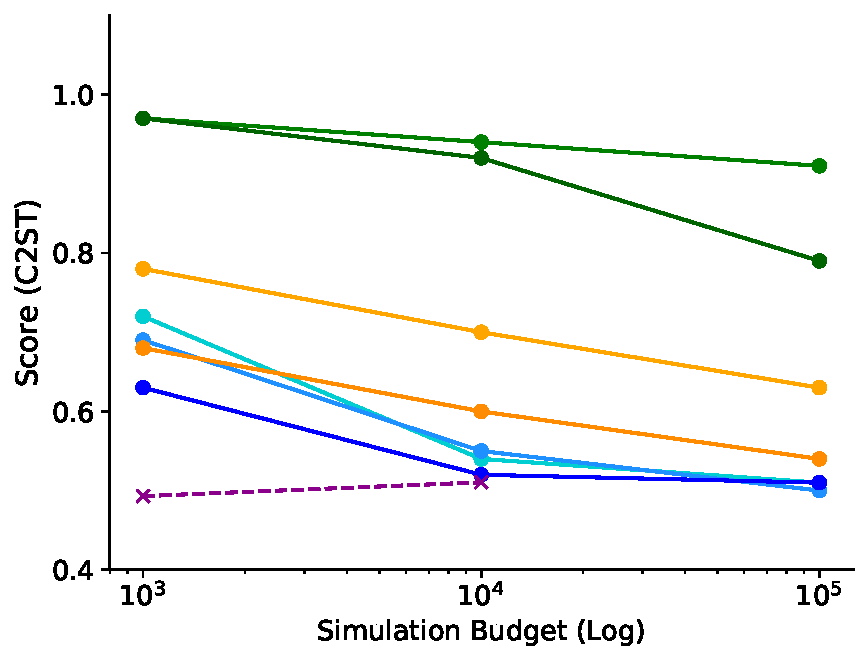
\includegraphics[width=.4\linewidth]{./figures/gaussian_linear_uniform.pdf}
%   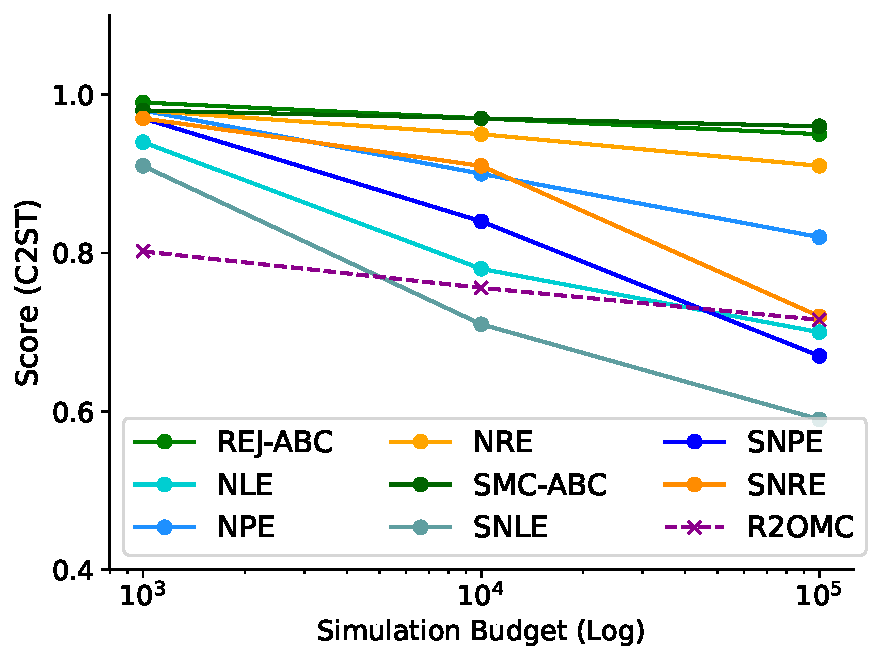
\includegraphics[width=.4\linewidth]{./figures/slcp.pdf}
%   \caption{Left---T.2: Gaussian Linear Uniform. Right---T.3: SLCP.}
%   \label{fig:exp_sbi_extra}
% \end{figure}

\subsection{MoG - Shifted Gaussian}

This additional experiment uses a simulator that samples from a mixture of two Gaussians, whose means are shifted by a constant value.

\begin{tabular}{@{}ll@{}}
  \textbf{Prior} & $\thb \sim \mathcal{U}(-15, 15)^4$ \\[5pt]
  \textbf{Simulator} & $\yb \sim \frac{1}{2} \left ( \mathcal{N}(\thb + \mathbf{5}, \mathbf{I}) + \mathcal{N}(\thb, \mathbf{I}) \right )$ \\[5pt]
  \textbf{Dimensionality} & $\thb \in \mathbb{R}^{4}$, $\yb \in \mathbb{R}^{4}$ \\[5pt]
\end{tabular}

We will use two separate cases: one with $N=4$ similar observations and another with $N=4$ different observations.
In both cases, the posterior is:
%
\begin{align}
  \label{eq:gauss_mult_obs}
  p(\thb|\{\data_n\}) &\propto p(\thb) p(\{\data_n\}|\thb) \\
                      &\propto p(\thb) \prod_{n=1}^{N} p(\data_n|\thb) \label{eq:gauss_mult_obs_1} \\
                      &\propto \mathcal{U}(-\mathbf{15},\mathbf{15}) \prod_{n=1}^{N} \dfrac{1}{2} \left ( \mathcal{N}(\data_n; \thb + \mathbf{5}, \mathbf{I}) + \mathcal{N}(\data_n; \thb, \mathbf{I}) \right ) \\
                      &\propto \mathcal{U}(-\mathbf{15},\mathbf{15}) \prod_{n=1}^{N} \dfrac{1}{2}\left ( \mathcal{N}(\thb; \data_n - \mathbf{5}, \mathbf{I}) + \mathcal{N}( \thb; \data_n, \mathbf{I}) \right ) \label{eq:gauss_mult_obs_3}\\
                      &\appropto \prod_{n=1}^{N} \left ( \mathcal{N}(\thb; \data_n - \mathbf{5}, \mathbf{I}) + \mathcal{N}( \thb; \data_n, \mathbf{I}) \right ) \label{eq:gauss_mult_obs_4}
\end{align}
In~(\ref{eq:gauss_mult_obs_1}), the factorization is due to the $N$ independently and identically distributed (iid) data points.
In~(\ref{eq:gauss_mult_obs_3}), we apply the property: $\mathcal{N}(\yb; \thb + \mub, \Sigma) = \mathcal{N}(\thb; \yb - \mub, \Sigma)$.
In~(\ref{eq:gauss_mult_obs_4}), we use that the data that we will use are sufficiently far from the boundaries so that we may ignore the boundary effects in the truncated distribution.

\paragraph{Case 1:}

In Case 1, we use $N=4$ similar observations: $\data_n \approx (0, \ldots, 0)$ for $n \in \{ 1, \ldots, N \}$. The ground-truth posterior is approximately:
%
\begin{equation}
  p(\thb | \data) \approx \mathcal{N}(\thb; - \mathbf{5}, \frac{1}{N} \mathbf{I}) + \mathcal{N}(\thb; \mathbf{0}, \frac{1}{N} \mathbf{I})
  \label{eq:mog_shifted_gaussian_case_1}
\end{equation}
%
\textbf{Proof.}
%
\begin{align} 
p(\thb|{\data_n}) 
&\appropto \prod_n^{N} \left ( \mathcal{N}(\thb; \data_n - \mathbf{5}, \mathbf{I}) + \mathcal{N}( \thb; \data_n, \mathbf{I}) \right ) \\
&\appropto \left( \mathcal{N}(\thb; - \mathbf{5}, \mathbf{I}) + \mathcal{N}(\thb; \mathbf{0}, \mathbf{I}) \right)^N \\
&\appropto \sum_{n=0}^N \binom{N}{n} (\mathcal{N}(\thb; - \mathbf{5}, \mathbf{I}))^n (\mathcal{N}(\thb; \mathbf{0}, \mathbf{I}))^{N-n} \\
&\appropto \left( \mathcal{N}(\thb; - \mathbf{5}, \mathbf{I}) \right)^N + \left( \mathcal{N}( \thb; \mathbf{0}, \mathbf{I}) \right)^N \label{eq:gauss_mult_obs_case_1_1}  \\
&\appropto \mathcal{N}(\thb; - \mathbf{5}, \frac{1}{N}\mathbf{I}) + \mathcal{N}( \thb; \mathbf{0}, \frac{1}{N}\mathbf{I}) \label{eq:gauss_mult_obs_case_1_2} 
\end{align}
%
In (\ref{eq:gauss_mult_obs_case_1_1}), for $n \in \{1, \ldots, N-1\}$ the terms involve products between 
$\mathcal{N}(\thb; - \mathbf{5}, \mathbf{I})$ and $ \mathcal{N}( \thb; \mathbf{0}, \mathbf{I})$ so they have 
a much smaller magnitude compared to $(\mathcal{N}(\thb; - \mathbf{5}, \mathbf{I}))^N$ ($n=N$) and $\mathcal{N}(( \thb; \mathbf{0}, \mathbf{I}))^N$ ($n=0$).
This allows us to approximate the expression by retaining only these two dominant terms.
In (\ref{eq:gauss_mult_obs_case_1_2}), we use the property that raising a Gaussian distribution to the power \(N\) results in a Gaussian with the same mean and a covariance scaled by \(\frac{1}{N}\). 
% In Figure~\ref{fig:multi_obs_case_1_gt} we show two dimensions, $\thb_i$ and $\thb_j$, of the ground truth posterior for $N=\{1, 4, 10, 20\}$ observations.

\paragraph{Case 2:}

In Case 2, we use an even number of $N$ observations that are split in two categories, 
half around $(0, \ldots, 0)$, i.e., 
$\data_n \approx (0, \ldots, 0)$ for $n \in \{ 1, \ldots, N/2 \}$ and the other half around 
$(5, \ldots, 5)$, i.e., 
$\data_n \approx (5, \ldots, 5)$ for $n \in \{ N/2 + 1, \ldots, N \}$.
The posterior, for values of $\thb$ sufficienty far from the boundary, is:
\begin{equation}
  p(\thb | \data) \approx \mathcal{N}(\thb; \mathbf{0}, \frac{1}{N} \mathbf{I})
  \label{eq:mog_shifted_gaussian_case_2}
\end{equation}

\textbf{Proof.}
\begin{align}
  p(\thb|\{\data_k\}) 
  &\appropto \prod_n^{N} \left ( \mathcal{N}(\thb; \data_n - \mathbf{5}, \mathbf{I}) + \mathcal{N}( \thb; \data_n, \mathbf{I}) \right ) \\
  &\appropto \prod_{n=1}^{N/2} \left ( \mathcal{N}(\thb; - \mathbf{5}, \mathbf{I}) + \mathcal{N}( \thb; \mathbf{0}, \mathbf{I}) \right ) \prod_{n=N/2 + 1}^{N} \left ( \mathcal{N}(\thb; \mathbf{0}, \mathbf{I}) + \mathcal{N}( \thb; \mathbf{5}, \mathbf{I}) \right )  \\
  &\appropto \prod_{n=1}^{N/2} \left ( \mathcal{N}(\thb; - \mathbf{5}, \mathbf{I}) + \mathcal{N}( \thb; \mathbf{0}, \mathbf{I}) \right ) \prod_{n=1}^{N/2} \left ( \mathcal{N}(\thb; \mathbf{0}, \mathbf{I}) + \mathcal{N}( \thb; \mathbf{5}, \mathbf{I}) \right )  \\
  &\appropto \left ( ( \mathcal{N}(\thb; - \mathbf{5}, \mathbf{I}) )^{N/2} + ( \mathcal{N}( \thb; \mathbf{0}, \mathbf{I}) )^{N/2} \right ) \left ( ( \mathcal{N}(\thb; \mathbf{0}, \mathbf{I}) )^{N/2} + ( \mathcal{N}( \thb; \mathbf{5}, \mathbf{I}) )^{N/2} \right ) \label{eq:gauss_mult_obs_case_2_1} \\
  &\appropto \mathcal{N}(\thb; \mathbf{0}, \mathbf{I})^N \label{eq:gauss_mult_obs_case_2_2} \\
  &\appropto \mathcal{N}( \thb; \mathbf{0}, \frac{1}{N}\mathbf{I}) \label{eq:gauss_mult_obs_case_2_3}
\end{align}
%
In (\ref{eq:gauss_mult_obs_case_2_1}), we keep only the dominant terms, as in Case 1.
In (\ref{eq:gauss_mult_obs_case_2_2}), we use that terms that involve combinations of \(\mathcal{N}(\thb; \mathbf{0}, \mathbf{I})^{N/2}\), \(\mathcal{N}(\thb; -\mathbf{5}, \mathbf{I})^{N/2}\) and \(\mathcal{N}(\thb; \mathbf{5}, \mathbf{I})^{N/2}\) have significantly smaller magnitudes compared to the dominant ones; \(\mathcal{N}(\thb; \mathbf{0}, \mathbf{I})^{N/2} \mathcal{N}(\thb; \mathbf{0}, \mathbf{I})^{N/2}\).
In (\ref{eq:gauss_mult_obs_case_2_3}), we use the property that raising a Gaussian distribution to the power \(N\) results in a Gaussian with the same mean and a covariance scaled by \(\frac{1}{N}\).
% In Figure~\ref{fig:multi_obs_case_2_gt} we show two dimensions, $\thb_i$ and $\thb_j$, of the ground truth posterior for $N=\{1, 4, 10, 20\}$ observations.

\paragraph{Results.}

Figure~\ref{fig:multi_obs} demonstrates that \rromc~aligns closely with the ground truth posterior, correctly capturing the two modes in Case 1 and the single mode in Case 2.
% Due to the approximation error introduced by $\epsilon$, \rromc~exhibits a slightly higher variance compared to the ground truth.
In contrast, both \romc~struggles with multiple observations, resulting in their samples being distributed along the \(45^{\circ}\) line.

\begin{figure}
    \centering
    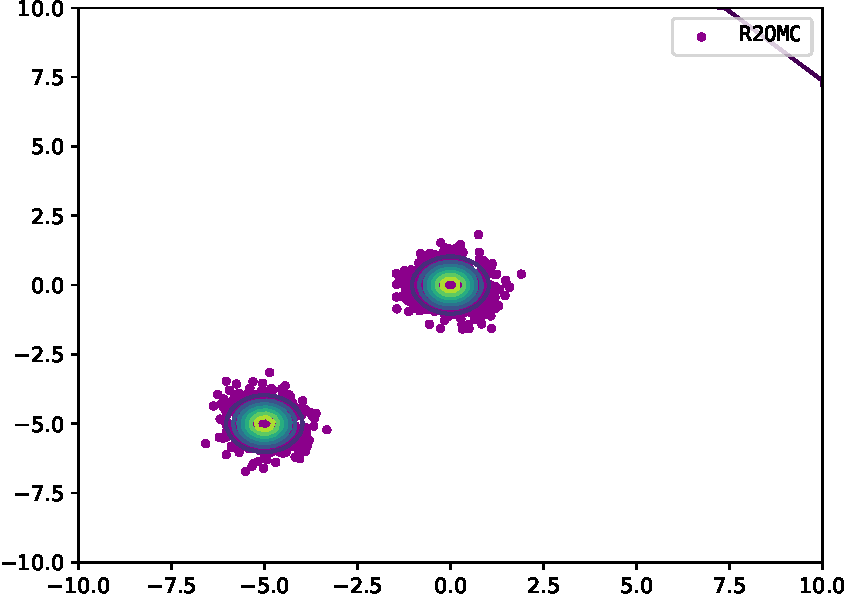
\includegraphics[width=0.23\linewidth]{figures/old/multi_obs_case_1_iterative_romc}
    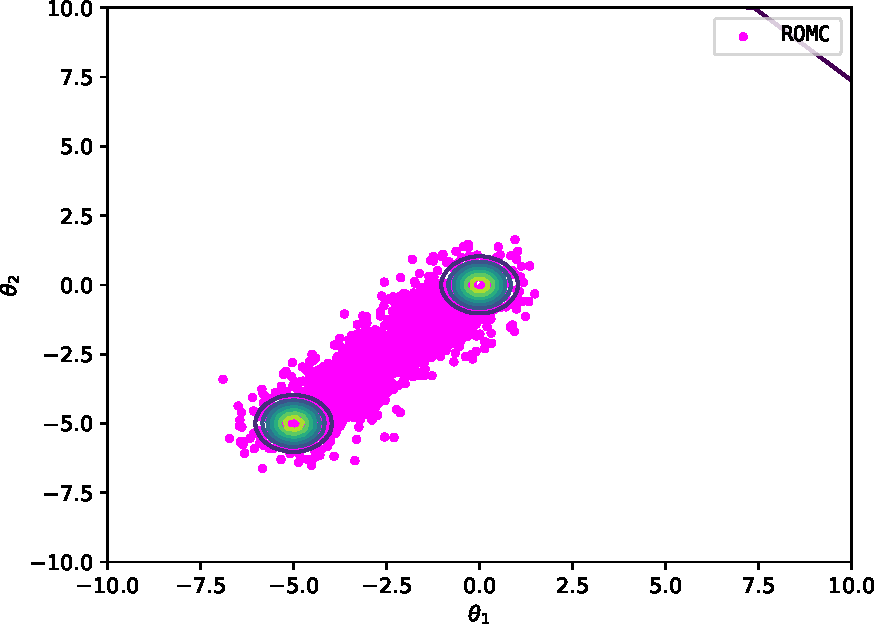
\includegraphics[width=0.23\linewidth]{figures/old/multi_obs_case_1_romc}
    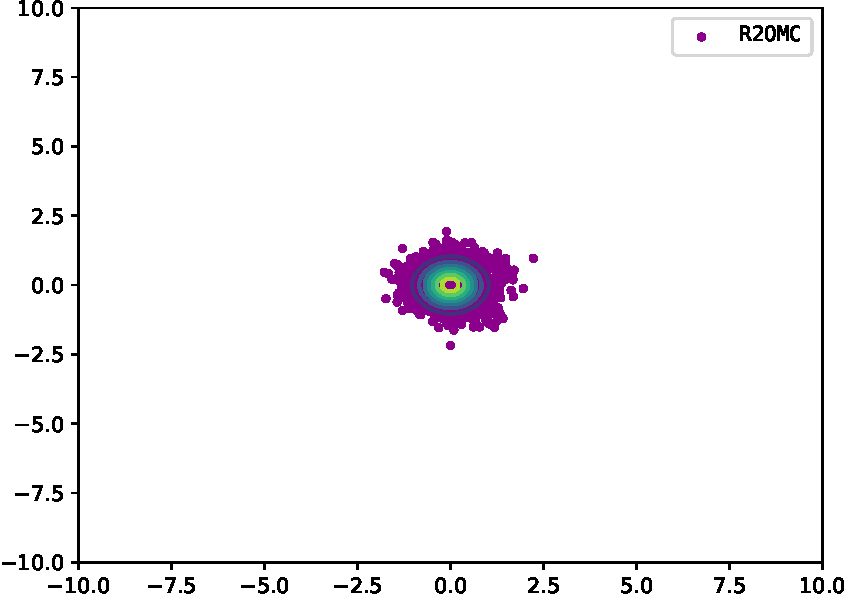
\includegraphics[width=0.23\linewidth]{figures/old/multi_obs_case_2_iterative_romc}
    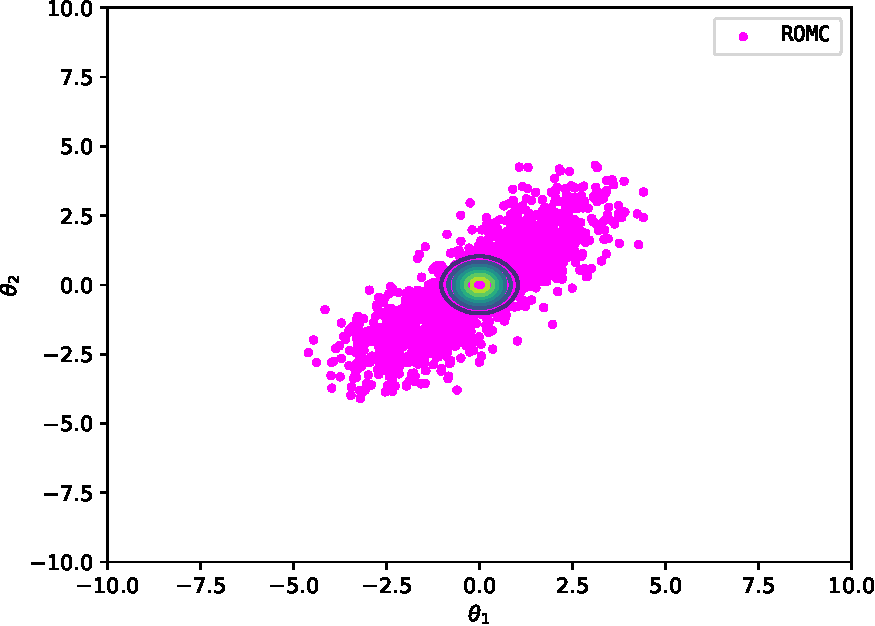
\includegraphics[width=0.23\linewidth]{figures/old/multi_obs_case_2_romc}
    \caption{From left to right: R2OMC on Case 1, Naive-ROMC on Case 1, R2OMC on Case 2, and Naive-ROMC on Case 2.}
    \label{fig:multi_obs}
\end{figure}


\end{document}
